% -*- mode: LaTeX; TeX-PDF-mode: t; -*-
\providecommand{\econtexRoot}{}
\renewcommand{\econtexRoot}{..}
\providecommand{\econtexPaths}{}\renewcommand{\econtexPaths}{\econtexRoot/Resources/econtexPaths}
% The \commands below are required to allow sharing of the same base code via Github between TeXLive on a local machine and Overleaf (which is a proxy for "a standard distribution of LaTeX").  This is an ugly solution to the requirement that custom LaTeX packages be accessible, and that Overleaf prohibits symbolic links

\providecommand{\econtex}{\econtexRoot/Resources/texmf-local/tex/latex/econtex}
\providecommand{\pdfsuppressruntime}{\econtexRoot/Resources/texmf-local/tex/latex/pdfsuppressruntime}
\providecommand{\econark}{\econtexRoot/Resources/texmf-local/tex/latex/econark}
\providecommand{\econtexSetup}{\econtexRoot/Resources/texmf-local/tex/latex/econtexSetup}
\providecommand{\econtexShortcuts}{\econtexRoot/Resources/texmf-local/tex/latex/econtexShortcuts}
\providecommand{\econtexBibMake}{\econtexRoot/Resources/texmf-local/tex/latex/econtexBibMake}
\providecommand{\econtexBibStyle}{\econtexRoot/Resources/texmf-local/bibtex/bst/econtex}
\providecommand{\econtexBib}{economics}
\providecommand{\economics}{\econtexRoot/Resources/texmf-local/bibtex/bib/economics}
\providecommand{\notes}{\econtexRoot/Resources/texmf-local/tex/latex/handout}
\providecommand{\handoutSetup}{\econtexRoot/Resources/texmf-local/tex/latex/handoutSetup}
\providecommand{\handoutShortcuts}{\econtexRoot/Resources/texmf-local/tex/latex/handoutShortcuts}
\providecommand{\handoutBibMake}{\econtexRoot/Resources/texmf-local/tex/latex/handoutBibMake}
\providecommand{\handoutBibStyle}{\econtexRoot/Resources/texmf-local/bibtex/bst/handout}

\providecommand{\FigDir}{\econtexRoot/Figures}
\providecommand{\CodeDir}{\econtexRoot/Code}
\providecommand{\DataDir}{\econtexRoot/Data}
\providecommand{\SlideDir}{\econtexRoot/Slides}
\providecommand{\TableDir}{\econtexRoot/Tables}
\providecommand{\ApndxDir}{\econtexRoot/Appendices}

\providecommand{\ResourcesDir}{\econtexRoot/Resources}
\providecommand{\rootFromOut}{..} % APFach back to root directory from output-directory
\providecommand{\LaTeXGenerated}{\econtexRoot/LaTeX} % Put generated files in subdirectory
\providecommand{\econtexPaths}{\econtexRoot/Resources/econtexPaths}
\providecommand{\LaTeXInputs}{\econtexRoot/Resources/LaTeXInputs}
\providecommand{\LtxDir}{LaTeX/}
\providecommand{\EqDir}{Equations} % Put generated files in subdirectory

\documentclass[BufferStockTheory]{subfiles}
% WARNING: AuCTeX local variables only get reset when file is loaded
% and differ between this file and BufferStockTheory.tex
% so must re-load whichever file you want to compile with C-x C-v

% WARNING: Different AucTeX execution depending on whether
% 0. Being compiled as standalone document
% * Compile main to completion
% * Then compile this one
% * Keep compiling until nothing changes
% 0. Being compiled as subfile of main document
% * Just compile main document repeatedly

\providecommand{\econtexRoot}{}
\renewcommand{\econtexRoot}{..}
\providecommand{\econtexPaths}{}\renewcommand{\econtexPaths}{\econtexRoot/Resources/econtexPaths}
% The \commands below are required to allow sharing of the same base code via Github between TeXLive on a local machine and Overleaf (which is a proxy for "a standard distribution of LaTeX").  This is an ugly solution to the requirement that custom LaTeX packages be accessible, and that Overleaf prohibits symbolic links

\providecommand{\econtex}{\econtexRoot/Resources/texmf-local/tex/latex/econtex}
\providecommand{\pdfsuppressruntime}{\econtexRoot/Resources/texmf-local/tex/latex/pdfsuppressruntime}
\providecommand{\econark}{\econtexRoot/Resources/texmf-local/tex/latex/econark}
\providecommand{\econtexSetup}{\econtexRoot/Resources/texmf-local/tex/latex/econtexSetup}
\providecommand{\econtexShortcuts}{\econtexRoot/Resources/texmf-local/tex/latex/econtexShortcuts}
\providecommand{\econtexBibMake}{\econtexRoot/Resources/texmf-local/tex/latex/econtexBibMake}
\providecommand{\econtexBibStyle}{\econtexRoot/Resources/texmf-local/bibtex/bst/econtex}
\providecommand{\econtexBib}{economics}
\providecommand{\economics}{\econtexRoot/Resources/texmf-local/bibtex/bib/economics}
\providecommand{\notes}{\econtexRoot/Resources/texmf-local/tex/latex/handout}
\providecommand{\handoutSetup}{\econtexRoot/Resources/texmf-local/tex/latex/handoutSetup}
\providecommand{\handoutShortcuts}{\econtexRoot/Resources/texmf-local/tex/latex/handoutShortcuts}
\providecommand{\handoutBibMake}{\econtexRoot/Resources/texmf-local/tex/latex/handoutBibMake}
\providecommand{\handoutBibStyle}{\econtexRoot/Resources/texmf-local/bibtex/bst/handout}

\providecommand{\FigDir}{\econtexRoot/Figures}
\providecommand{\CodeDir}{\econtexRoot/Code}
\providecommand{\DataDir}{\econtexRoot/Data}
\providecommand{\SlideDir}{\econtexRoot/Slides}
\providecommand{\TableDir}{\econtexRoot/Tables}
\providecommand{\ApndxDir}{\econtexRoot/Appendices}

\providecommand{\ResourcesDir}{\econtexRoot/Resources}
\providecommand{\rootFromOut}{..} % APFach back to root directory from output-directory
\providecommand{\LaTeXGenerated}{\econtexRoot/LaTeX} % Put generated files in subdirectory
\providecommand{\econtexPaths}{\econtexRoot/Resources/econtexPaths}
\providecommand{\LaTeXInputs}{\econtexRoot/Resources/LaTeXInputs}
\providecommand{\LtxDir}{LaTeX/}
\providecommand{\EqDir}{Equations} % Put generated files in subdirectory

\onlyinsubfile{% https://tex.stackexchange.com/questions/463699/proper-reference-numbers-with-subfiles
    \csname @ifpackageloaded\endcsname{xr-hyper}{%
      \externaldocument{\econtexRoot/BufferStockTheory}% xr-hyper in use; optional argument for url of main.pdf for hyperlinks
    }{%
      \externaldocument{\econtexRoot/BufferStockTheory}% xr in use
    }%
    \renewcommand\labelprefix{}%
    % Initialize the counters via the labels belonging to the main document:
    \setcounter{equation}{\numexpr\getrefnumber{\labelprefix eq:Dummy}\relax}% eq:Dummy is the last number used for an equation in the main text; start counting up from there
}


\onlyinsubfile{\externaldocument{BufferStockTheory}} % Get xrefs -- esp to apndx -- from main file; only works if main file has already been compiled

% % Redefine commands from sty file to signal compilation from master

\newcommand{\thankstext}{
  The paper's results \href{https://\owner.github.io/nbreproduce}{can be automatically reproduced} using the {\ARKurl} toolkit, which can be cited per our references (\cite{carroll_et_al-proc-scipy-2018}); for reference to the toolkit itself see \href{https://econ-ark.org/acknowledging}{Acknowledging Econ-ARK}.  Thanks to the \href{https://consumerfinance.gov}{Consumer Financial Protection Bureau} for funding the original creation of the {\ARKurl} toolkit; and to the \href{https://sloan.org}{Sloan Foundation} for funding Econ-ARK's \href{https://sloan.org/grant-detail/8071}{extensive further development} that brought it to the point where it could be used for this project.  The toolkit can be cited with its digital object identifier, \href{https://doi.org/10.5281/zenodo.1001067}{10.5281/zenodo.1001067}, as is done in the paper's own references as \cite{carroll_et_al-proc-scipy-2018}.  Thanks to Will Du, James Feigenbaum, Joseph Kaboski, Miles Kimball, Qingyin Ma, Misuzu Otsuka, Damiano Sandri, John Stachurski, Adam Szeidl, Alexis Akira Toda, Metin Uyanik, Mateo Vel\'asquez-Giraldo, Weifeng Wu,  Jiaxiong Yao, and Xudong Zheng for comments on earlier versions of this paper, John Boyd for help in applying his weighted contraction mapping theorem, Ryoji  Hiraguchi for extraordinary mathematical insight that improved the  paper greatly, David Zervos for early guidance to the literature, and participants in a seminar at the Johns Hopkins University, a presentation at the 2009 meetings of the Society of Economic Dynamics for their insights, and at a presentation at the Australian National University.}

% \newcommand{\inframe}{https://\owner.github.io/BufferStockTheory/BufferStockTheory3.html}

% Embed metadata
\hypersetup{pdfauthor={Christopher D. Carroll <ccarroll@jhu.edu>},
  pdftitle={Theoretical Foundations of Buffer Stock Saving},
  pdfkeywords={Precautionary saving, buffer-stock saving, consumption, marginal propensity to consume, permanent income hypothesis, income fluctuation problem},
  pdfnewwindow=true,
  pdfcreator = {ccarroll@jhu.edu}
}

\begin{document}

% Attempted to make all lines used for Web version contain {Web} (or version with only single curly brace at end) so can be removed with sed
\ifthenelse{\boolean{Web}}{    % {Web}
  \renewcommand{\versn}{Web}     % Too hard to figure out passing -output-directory through make4ht through htlatex, so web version is compiled with junk files in main directory
  \renewcommand{\rootFromOut}{.} % {Web}
}{}  % {Web}


% Tiny info header at top tracks git commit
%\hfill{\tiny \jobname~\versn~\today~{at} \DTMcurrenttime, \input{\ResourcesDir/.git-source-commit}~~\input{\ResourcesDir/.git-public-commit}}

\title{Theoretical Foundations of \\ Buffer Stock Saving}

\author{Christopher D. Carroll\authNum}

\keywords{Precautionary saving, buffer stock saving, marginal propensity to consume, permanent income hypothesis, income fluctuation problem}

\jelclass{D81, D91, E21 \par
  \href{https://econ-ark.org}{
\includegraphics{\ResourcesDir/PoweredByEconARK}}
}

% \date{\today}
\renewcommand{\forcedate}{November 10, 2022}\date{\forcedate}

\maketitle
\hypertarget{abstract}{}
\begin{abstract}
  This paper builds foundations for rigorous and intuitive understanding of `buffer stock' saving models (\cite{bewleyPIH}-like models with a wealth target), pairing each theoretical result with quantitative illustrations.  After describing conditions under which a consumption function exists, the paper articulates stricter `Growth Impatience' conditions that guarantee alternative forms of stability --- either at the population level, or for individual consumers.  Together, the numerical tools and analytical results constitute a comprehensive toolkit for understanding buffer stock models.
\end{abstract}

% Various resources
\hypertarget{links}{}

\newcommand{\REMARK}{\href{https://github.com/econ-ark/REMARK}{REMARK}}
\begin{footnotesize}
  \parbox{0.9\textwidth}{
    \begin{center}
      \begin{tabbing}
        \texttt{~~~\REMARK:~} \= \= \texttt{\url{https://econ-ark.org/materials/bufferstocktheory}} \\ 
        \texttt{Dashboard:~} \> \> \texttt{\href{https://econ-ark.org/materials/bufferstocktheory}{Click `Launch Dashboard' Button}} \\
        \texttt{~~~~~html:~} \> \> \texttt{\href{https://\owner.github.io/BufferStockTheory/}{https://\owner.github.io/BufferStockTheory/}} \\ % Owner is defined in Resources/owner.tex
        \texttt{~~~~~~PDF:~} \> \> \texttt{\href{https://github.com/\owner/BufferStockTheory/blob/master/LaTeX/BufferStockTheory.pdf}{BufferStockTheory.pdf}} \\ 
        \texttt{~~~Slides:~} \> \> \texttt{\href{https://github.com/\owner/BufferStockTheory/blob/master/LaTeX/BufferStockTheory-Slides.pdf}{BufferStockTheory-Slides.pdf}} \\
%        \texttt{~Appendix:~} \> \> \texttt{\url{https://\owner.github.io/BufferStockTheory/BufferStockTheory3.html#Appendices}}    \\
        \texttt{~~~GitHub:~} \> \> \texttt{\href{https://github.com/\owner/BufferStockTheory}{https://github.com/\owner/BufferStockTheory}} \\
      \end{tabbing}
    \end{center}
    % The \href{https://econ-ark.org/materials/bufferstocktheory\?dashboard}{dashboard} lets users see consequences of alternative parameters in an interactive framework.
  } % end \parbox{\textwidth}
\end{footnotesize}

\begin{authorsinfo}
  \name{Contact: \href{mailto:ccarroll@jhu.edu}{\texttt{ccarroll@jhu.edu}}, Department of Economics, 590 Wyman Hall, Johns Hopkins University, Baltimore, MD 21218, \url{https://www.econ2.jhu.edu/people/ccarroll}, and National Bureau of Economic Research.}
\end{authorsinfo}

\pagenumbering{gobble} % Prevent numbering for pages including the TOC and title page


\ifthenelse{\boolean{Web}}{
}{
  \begin{minipage}{0.9\textwidth}
    \footnotesize The paper's results \href{https://\owner.github.io/nbreproduce}{can be automatically reproduced} using the {\ARKurl} toolkit by executing the \href{https://econ-ark.org/materials/bufferstocktheory}{notebook}; for reference to the toolkit itself see \href{https://econ-ark.org/acknowledging}{Acknowleding Econ-ARK}.  Thanks to the \href{https://consumerfinance.gov}{Consumer Financial Protection Bureau} for funding the original creation of the {\ARKurl} toolkit; and to the \href{https://sloan.org}{Sloan Foundation} for funding Econ-ARK's \href{https://sloan.org/grant-detail/8071}{extensive further development} that brought it to the point where it could be used for this project.  The toolkit can be cited with its digital object identifier, \href{https://doi.org/10.5281/zenodo.1001067}{https://doi.org/10.5281/zenodo.1001067}, as is done in the paper's own references as \cite{carroll_et_al-proc-scipy-2018}.  Thanks to Will Du, James Feigenbaum, Joseph Kaboski, Miles Kimball, Qingyin Ma, Misuzu Otsuka, Damiano Sandri, John Stachurski, Adam Szeidl, Alexis Akira Toda, Metin Uyanik, Mateo Vel\'asquez-Giraldo, Weifeng Wu,  Jiaxiong Yao, and Xudong Zheng for comments on earlier versions of this paper, John Boyd for help in applying his weighted contraction mapping theorem, Ryoji  Hiraguchi for extraordinary mathematical insight that improved the  paper greatly, David Zervos for early guidance to the literature, and participants in a seminar at the Johns Hopkins University, a presentation at the 2009 meetings of the Society of Economic Dynamics for their insights, and at a presentation at the Australian National University.
  \end{minipage}

  \titlepagefinish\pagebreak
  \let\LaTeXStandardContentsName\contentsname
  \renewcommand{\contentsname}{}
  \tableofcontents
  \pagebreak

  \medskip\medskip
  \begin{minipage}{0.9\textwidth}
    \listoffigures 
  \end{minipage}

  \medskip\medskip
  \begin{minipage}{0.9\textwidth}
    \listoftables
  \end{minipage}
} % {Web}
\pagebreak
\hypertarget{Introduction}{}
\section{Introduction}\label{sec:intro}
\setcounter{page}{0}\pagenumbering{arabic}

For consumers whose income is affected by realistic transitory and permanent shocks (\textit{a la}~\cite{friedmanATheory} and~\cite{muthOptimal}), only one further ingredient is required to construct a microeconomically testable model of optimal consumption: A description of preferences.  \cite{zeldesStochastic} was the first to calibrate a quantitatively plausible example, spawning a literature showing that such models' predictions can match household life cycle data reasonably well, whether or not explicit liquidity constraints are imposed.\footnote{See~\cite{carrollBSLCPIH} or~\cite{gpLifeCycle} for arguments that models with only `natural' constraints (see below) match a wide variety of facts; for a model with explicit constraints that produces very similar results, see, e.g.~\cite{Cagetti}.}

A connected literature, starting with~\cite{bewleyPIH}, has derived limiting properties of related infinite-horizon problems -- but only in models more complex than the case with just Friedman-Muth shocks and preferences, because standard contraction mapping theorems (from \cite{bellmanDynamicProgramming} through Stokey et~al.~\citeyearpar{slpMethods} and beyond) cannot be applied when utility and/or marginal utility are unbounded, and many proof methods rule out Friedman-Muth permanent shocks.\footnote{See \hyperlink{DiffFromLit}{the fuller discussion} at the end of Section~\ref{subsec:Setup}.}

This paper's first contribution is to articulate conditions under which the infinite-horizon Friedman-Muth(-Zeldes) problem (with permanent shocks, and without complications like a consumption floor or liquidity constraints) defines a contraction mapping whose limit is \hyperlink{useful}{useful} (neither $c=0$ nor $c=\infty$ everywhere) as the horizon recedes.  As in the more complicated models, a \hyperlink{FVAC}{`Finite Value of Autarky Condition'} is mostly sufficient (the \hyperlink{WRIC}{`Weak Return Impatience Condition'}\footnote{This is a generalization of a condition in~\cite{mstIncFluct}.} is unlikely to bind).  Because the infinite-horizon solution is the limit of finite-horizon recursions, many results are also applicable to finite-horizon problems.

But the main theoretical contribution is to identify, for the infinite-horizon case, conditions under which `stable' points exist (the ratio of wealth to permanent income will move toward a `target'; alternatively, there is a `balanced growth' equilibrium) either for individual consumers or for the aggregate.  The requirement for stability is always that the model's parameters satisfy a `Growth Impatience Condition' whose details depend on the quantity whose stability is of interest.  A model with any such stable point(s) qualifies as a `buffer stock' model.  (Buffer stock models are neither a subset nor a superset of~\cite{bewleyPIH} models).\footnote{(See the literature discussion below; Bewley models traditionally do not allow permanent shocks, and do not definitionally require existence of `stable' points (though such points will often exist).}

\hypertarget{KMP}{} Even without a formal proof of its existence, buffer stock saving has been intuitively understood to underlie key results in heterogeneous agent macroeconomics; for example, the logic of target saving is central to the claim by~\cite{kmpHandbook} in the \textit{Handbook of Macroeconomics} that such models explain why, during the Great Recession, middle-class consumers cut their spending more than the poor or the rich.  Theory below provides the rigorous basis for this claim:  Learning that the future has become more uncertain does not change the urgent imperatives of the poor (their high $\uFunc^{\prime}(\cNrm)$ means they --- optimally --- have little room to maneuver).  And, increased labor income uncertainty does not much change the behavior of the rich because it poses little risk to their consumption.  Only people in the middle have both the motivation and the wiggle-room to respond to uncertainty by substantially reducing their spending.  Analytical derivations required for the proofs also provide intuition for many other results familiar from the numerical literature.

The paper begins by describing sufficient conditions for the problem to define a \hyperlink{sensible}{sensible} (nondegenerate) limiting consumption function (while explaining how the model relates to those previously considered).  The conditions are interestingly parallel to those required for the \hyperlink{Factors-Defined-And-Compared}{liquidity constrained perfect foresight model}; that parallel is explored and explained.  The limiting properties of the consumption function as resources approach infinity, and as they approach their lower bound, are then used to prove the contraction mapping theorem.

The next theoretical contribution is to show that a model with an `artificial' liquidity constraint (it prohibits borrowing by consumers who could certainly repay) is a limiting case of the unconstrained model.  The analytical appeal of the unconstrained model is that it is both mathematically convenient (the consumption function is everywhere twice continuously differentiable), and arbitrarily close (cf.\ Section~\ref{sec:deatonIsLimit}) to less tractable models. This congenial environment makes proofs easier (if we define a proposition as holding in the infinite-horizon limit when it holds as a finite horizon extends to infinity).

In proving the remaining theorems, the \hyperlink{AnalysisoftheConvergedConsumptionFunction}{next section} examines key properties of the model. First, \hyperlink{LimitsAsmtToInfty}{as cash approaches infinity} the expected growth rate of consumption and the marginal propensity to consume (MPC) converge to their values in the perfect foresight case. Second, \hyperlink{LimitsAsmtToZero}{as cash approaches zero} the expected growth rate of consumption approaches infinity, and the MPC approaches a simple analytical limit.  Next, the central theorems articulate conditions under which different measures of `growth impatience' imply conclusions about points of stability (`target' or `balanced growth' points).

The final section elaborates the conditions under which, even with a fixed aggregate interest rate that differs from the time preference rate, a small open economy populated by buffer stock consumers has a balanced growth equilibrium in which growth rates of consumption, income, and wealth match the exogenous growth rate of permanent income (equivalent, here, to productivity growth). In the terms of~\cite{schmitt2003closing}, buffer stock saving is an appealing method of `closing' a small open economy, because it requires no \textit{ad-hoc} assumptions.  Not even liquidity constraints.\footnote{The paper's insights are instantiated in the {\ARKurl} toolkit, whose \href{https://hark.readthedocs.io/en/stable/reference/ConsumptionSaving/ConsIndShockModel.html}{buffer stock saving module} flags parametric choices under which a problem is degenerate or under which stable ratios of wealth to income may not exist.}

% Keep track of where you are via header at top of PDF
\ifthenelse{\boolean{Web}}{}{% else
  \automark{subsection}
} % {Web}

\hypertarget{The-Problem}{}
\section{The Problem}
\subsection{Setup}\label{subsec:Setup}

The infinite horizon solution is the (limiting) first-period solution to a sequence of finite-horizon problems as the horizon (the last period of life) becomes arbitrarily distant.

\hypertarget{sensible}{}\hypertarget{useful}{}
That is, for the value function, fixing a terminal date $T$,  we are interested in $\vLvl_{T-n}$ in the sequence of value functions $\{\vLvl_{T},\vLvl_{T-1},\ldots,\vLvl_{T-n}\}$.  We will say that the problem has a `nondegenerate' infinite horizon solution if, corresponding to that $\vLvl$, as $n \uparrow \infty$ there is a limiting consumption function $\usual{\cLvl}(\mLvl,\pLvl) = \lim_{n \uparrow \infty} \cLvl_{T-n}(\mLvl,\pLvl)$ which is neither $\usual{\cLvl}=0$ everywhere (for all $\mLvl,\pLvl$) nor $\usual{\cLvl}=\infty$ everywhere (a `sensible' solution).

Concretely, a consumer born $n$ periods before date $T$ solves the problem\footnote{Notation throughout follows guidelines specified for the {\ARKurl} toolkit; see \href{https://github.com/econ-ark/HARK/blob/master/Documentation/NARK/NARK.pdf}{Notation in the ARK} for rationales and details.  (Consequently, there is an exact mapping between objects in the paper and objects in the code.)}
\begin{verbatimwrite}{\EqDir/supfn}
  \begin{align*}
    \vLvl_{T-n} & = \max~ \Ex_{t}\left[\sum_{i=0}^{n} \DiscFac^{i} \uFunc(\cLvl_{t+i})\right]
  \end{align*}
\end{verbatimwrite}
  \begin{align*}
    \vLevBF_{T-n} & = \max~ \Ex_{t}\left[\sum_{i=0}^{n} \DiscFac^{i} \uFunc(\cLevBF_{t+i})\right]
  \end{align*}

where the Constant Relative Risk Aversion (CRRA) utility function
\begin{align*}
  \uFunc(\bullet)=\bullet^{1-\CRRA}/(1-\CRRA) 
\end{align*}
exhibits relative risk aversion $\CRRA > 1$.\footnote{The main results also hold for logarithmic utility which is the limit as $\CRRA \rightarrow 1$ but incorporating the logarithmic special case in the proofs is omitted because it would be cumbersome.}  The consumer's initial condition is defined by market resources $\mLvl_{t}$ and permanent noncapital income $\PermLvl_{t}$, which both are positive,
\begin{align}
  \{\PermLvl_{t},\mLvl_{t}\} & \in (0,\infty) \label{eq:PermLvlandmLvlgt0},
\end{align}
and the consumer cannot die in debt,
\begin{align}
  \cLvl_{T} & \leq  \mLvl_{T} \label{eq:NoDebtAtDeath}.
\end{align}

\hypertarget{checkRestrictions}{}
\hypertarget{DBCparts}{}
In the usual exposition, a dynamic budget constraint (DBC) combines several distinct events that jointly determine next period's $\mLvl_{t+1}$ (given this period's choices); for the detailed analysis here, we disarticulate and describe every separate step:\footnote{The steps are broken down also so that the notation of the paper will correspond exactly to the variable names in the \href{https://github.com/econ-ark/HARK} toolkit.}$^{,}$\footnote{Allowing a stochastic interest factor would complicate the notation but not affect the points we want to address; however, see~\cite{benhabibWealth},~\cite{maTodaRich}, and~\cite{mstIncFluct} for the implications of capital income risk for the distribution of wealth and other interesting questions not considered here.}
\begin{verbatimwrite}{\EqDir/DBCparts}
  \begin{equation}\iflabelexists{eq:DBCparts}{}{\label{eq:DBCparts}} % Don't define it if already defined
    \begin{split}
      \aLvl_{t}     & = \mLvl_{t}-\cLvl_{t}  
      \\     \kLvl_{t+1}   & = \aLvl_{t} \notag
      \\      \bLvl_{t+1}    & = \kLvl_{t+1} \Rfree \notag \\
      \PermLvl_{t+1}  & = \PermLvl_{t} \underbrace{\PermGroFac\PermShk_{t+1}}_{\equiv \PermGroFac_{t+1}} \notag \\
      \mLvl_{t+1}  & =  \bLvl_{t+1} +\PermLvl_{t+1}\TranShkAll_{t+1},\notag
    \end{split}
  \end{equation}
\end{verbatimwrite}
  \begin{equation}\iflabelexists{eq:DBCparts}{}{\label{eq:DBCparts}} % Don't define it if already defined
    \begin{split}
      \aLvl_{t}     & = \mLvl_{t}-\cLvl_{t}
      \\     \kLvl_{t+1}   & = \aLvl_{t} \notag
      \\      \bLvl_{t+1}    & = \kLvl_{t+1} \Rfree \notag \\
      \PermLvl_{t+1}  & = \PermLvl_{t} \underbrace{\PermGroFac\PermShk_{t+1}}_{\equiv \PermGroFac_{t+1}} \notag \\
      \mLvl_{t+1}  & =  \bLvl_{t+1} +\PermLvl_{t+1}\TranShkAll_{t+1},\notag
    \end{split}
  \end{equation}

\noindent where $\aLvl_{t}$ measures the consumer's assets at the end of $t$, which translate one-for-one into capital $\kLvl_{t+1}$ at the beginning of the next period. Before the consumption choice, $\kLvl_{t+1}$ is augmented by a fixed interest factor $\Rfree =(1+\rfree)$ to become $\bLvl_{t+1}$ -- the consumer's financial (`\textbf{b}ank') balances before next period's consumption choice; $\mLvl_{t+1}$ (`market resources') is the sum of financial wealth $\bLvl_{t+1}$ and noncapital income $\PermLvl_{t+1}\TranShkAll_{t+1}$ (permanent noncapital income $\PermLvl_{t+1}$ multiplied by the transitory-income-shock factor $\TranShkAll_{t+1}$ described below). $\pLvl_{t+1}$ is derived from $\pLvl_{t}$ via application of a growth factor $\PermGroFac$,\footnote{This could be made IID stochastic with straightforward consequences for any of the analysis below; this is an option in the \href{https://econ-ark.org}{HARK} toolkit.} modified by a mean-one iid shock $\PermShk_{t+1}$, $\Ex_{t}[{\PermShk}_{t+n}]=1~\forall~n \geq 1$ satisfying $\PermShk \in [\ushort{\PermShk},\bar{\PermShk}]$ for $0 < \ushort{\PermShk} \leq 1 \leq \bar{\PermShk} < \infty$ (and $\ushort{\PermShk}=\bar{\PermShk}=1$ is the degenerate case with no permanent shocks).

Following~\cite{zeldesStochastic}, in future periods $t+n~\forall~n \geq 1$ there is a small probability $\pZero$ that income will be zero (a `zero-income event'),
\begin{verbatimwrite}{\EqDir/TranShkDef}
  \begin{equation}
    \TranShkAll _{t+n}=
    \begin{cases}
      0\phantom{_{t+1}/\pNotZero} & \text{with probability $\pZero>0$} \\
      \TranShkEmp_{t+n}/\pNotZero      & \text{with probability $\pNotZero  $} % \equiv (1-\pZero)
    \end{cases} \label{eq:TranShkDef}
  \end{equation}
\end{verbatimwrite}
  \begin{equation}
    \TranShkAll _{t+n}=
    \begin{cases}
      0\phantom{_{t+1}/\pNotZero} & \text{with probability $\pZero>0$} \\
      \TranShkEmp_{t+n}/\pNotZero      & \text{with probability $\pNotZero  $} % \equiv (1-\pZero)
    \end{cases} \label{eq:TranShkDef}
  \end{equation}
 %
where $\TranShkEmp_{t+n}$ is an iid mean-one random variable ($\Ex_{t}[{\TranShkEmp}_{t+n}]=1~\forall~n>0$) whose distribution satisfies $\TranShkEmp \in \lbrack \ushort{\TranShkEmp},\bar{\TranShkEmp}\rbrack$ where $0<\ushort{\TranShkEmp} \leq 1 \leq \bar{\TranShkEmp}<\infty$.\footnote{\cite{rabaultBorrowing} and~\cite{lsIncFluct} analyze cases where the shock processes have unbounded support.}  Call the cumulative distribution functions $\CDF_{\PermShk}$ and $\CDF_{\TranShkEmp}$ (where $\CDF_{\TranShkAll}$ is derived trivially from~\eqref{eq:TranShkDef} and $\CDF_{\TranShkEmp}$).  For quick identification in tables and graphs, we will call this the `Friedman/Muth' model because it is a specific implementation of~\cite{friedmanATheory}'s ideas as interpreted by~\cite{muthOptimal}.


\hypertarget{PDV}{}

The model looks more special than it is.  In particular, a positive probability of zero-income events may seem objectionable (despite empirical support).\footnote{We calibrate this probability to 0.005 to match data from the Panel Study of Income Dynamics (\cite{carrollBrookings}).}  But a nonzero minimum value of $\TranShkAll$ (motivated, say, by the existence of unemployment insurance) could be handled by capitalizing the PDV of minimum income into current market assets,\footnote{So long as unemployment benefits are proportional to $\PermLvl_{t}$; see the discussion in Section~\ref{sec:discussConvergence}.}  transforming that model back into this one.  And no key results would change if the transitory shocks were persistent but mean-reverting (instead of IID).\@ Also, the assumption of a positive point mass for the worst realization of the transitory shock is inessential, but simplifies the proofs and is a powerful aid to intuition.%\footnote{A positive density over a positive interval above the lower bound would work instead but would be cumbersome.}

\hypertarget{cfLiterature}{}
\subsection{Comparison to Existing Literature}\label{subsec:Lit}
\hypertarget{DiffFromLit}{} This model differs from Bewley's~\citeyearpar{bewleyPIH} classic formulation in several ways. The CRRA utility function does not satisfy Bewley's assumption that $\uFunc(0)$ is well-defined, or that $\uP(0)$ is well-defined and finite; indeed, neither the value function nor the marginal value function will be bounded.  It differs from Schectman and Escudero~\citeyearpar{seIncFluct} in that they impose liquidity constraints and positive minimum income.  It differs from both of these in that it permits permanent growth in income, and also permanent shocks to income, which a large empirical literature finds to be of dominant importance in microdata.\footnote{MaCurdy~\citeyearpar{macurdyTimeseries}; Abowd and Card~\citeyearpar{acCovariance}; Carroll and Samwick~\citeyearpar{csNature}; Jappelli and Pistaferri~\citeyearpar{jpCins}; et. seq.  Much of the literature instead incorporates highly `persistent' but not completely permanent shocks, but~\cite{dhmImproving} show that when measurement problems are handled correctly, admin data yield serial correlation coefficients $0.98-1.00$; and~\cite{dmHowMuch} suggests that survey data support the same conclusion.}  It differs from Deaton~\citeyearpar{deatonLiqConstr} because liquidity constraints are absent; there are separate transitory and permanent shocks (\textit{a la}~\cite{muthOptimal}); and the transitory shocks here can occasionally cause income to reach zero.

It differs from models found in Stokey et.\ al.~\citeyearpar{slpMethods} because neither liquidity constraints nor bounds on utility or marginal utility are imposed.\footnote{Similar restrictions are made in the well known papers by Scheinkman and Weiss~\citeyearpar{scheinkman&weiss:borrowing}, Clarida~\citeyearpar{claridaErgodic}, and~\cite{cwcUnderUncert}.  See~\cite{tocheUrisk} for elegant analysis of a related but simpler continuous-$t$ model.}$^{,}$\footnote{\cite{asHomogeneous} relaxed the bounds on the return function, but they address only the deterministic case.}~\cite{lsIncFluct} show how to allow unbounded returns by using policy function iteration, but also impose constraints.

The paper with perhaps the most commonalities is~\cite{mstIncFluct}, henceforth MST, who establish existence and uniqueness of a solution to a general income fluctuation problem in a Markovian setting.  The most important differences are that MST impose liquidity constraints and that expected marginal utility of income is finite ($\Ex[\uFunc^{\prime}(Y)]<\infty)$.  These assumptions are not consistent with the combination of CRRA utility and income dynamics used here, whose joint properties are key to the results.\footnote{The incorporation of permanent shocks rules out application of the tools of~\cite{mnUnique}, who followed and corrected an error in the fundamental work on the local contraction mapping method developed in~\cite{rrExistence}.\@~\cite{mvExistence} provide a correction to~\cite{rrExistence}, that works under easier conditions to verify, but only addresses the deterministic case.}

\hypertarget{The-Problem-Can-Be-Rewritten-in-Ratio-Form}{}
\hypertarget{The-Problem-Can-Be-Normalized-By-Permanent-Income}{}
\subsection{The Problem Can Be Normalized By Permanent Income}\label{subsec:ratio}

We establish a bit more notation by reviewing the familiar result that in such problems (CRRA utility, permanent shocks) the number of states can be reduced from two ($\mLvl$ and $\PermLvl$) to one $(\mNrm = \mLvl/\PermLvl)$.  Value in the last period is $\uFunc(\mLvl_{T})$; using (in the last line in~\eqref{eq:vBold}) the fact that for our CRRA utility function, $\uFunc(xy) = x^{1-\CRRA}\uFunc(y)$, and generically defining nonbold variables as the boldface counterpart normalized by $\PermLvl_{t}$ (as with $\mNrm=\mLvl/\PermLvl$), consider the problem in the second-to-last period,
\begin{equation}\label{eq:vBold}
  \begin{split}
    \vLvl_{T-1}(\mLvl_{T-1},\PermLvl_{T-1})
    & =  \max_{\cNrm_{T-1}}~
    \uFunc(\PermLvl_{T-1}\cNrm_{T-1}) + \DiscFac  \Ex_{T-1} [\uFunc(\PermLvl_{T}{\mNrm}
    _{T})]  \\
    & = \PermLvl_{T-1}^{1-\CRRA}
    \left\{\max_{\cNrm_{T-1}}~ \uFunc(c_{T-1}) + \DiscFac \Ex_{T-1} [ \uFunc( {\PermGroFac}_{T}
      {\mNrm}_{T}) ] \right\}.
  \end{split}
\end{equation}

\hypertarget{The-Related-Problem}{}

Now, in a one-time deviation from the notational convention established in the last sentence, define nonbold `normalized value' not as $\vLvl_{t}/\PermLvl_{t}$ but as $\vFunc_{t} = \vLvl_{t}/\PermLvl_{t}^{1-\CRRA}$, because this allows us to exploit features of the related problem,
\begin{equation}\label{eq:veqn}
  \begin{split}
    % \begin{align*}
    \vFunc_{t}(\mNrm_{t})  & = \max_{{\{\cFunc\}}_{t}^{T}}~  \uFunc(\cFunc_{t}) +\DiscFac \Ex_{t}[\PermGroFac_{t+1}^{1-\CRRA}\vFunc_{t+1}({\mNrm}_{t+1})]  \\
    & \mbox{s.t.}
    \\ {\aNrm}_{t}  & = \mNrm_{t}-c_{t}
    \\ {\kNrm}_{t+1} & = \aNrm_{t}/\PermGroFac_{t+1}
    \\ {\bNrm}_{t+1}  & = {\kNrm}_{t+1}\Rfree = (\Rfree/\PermGroFac_{t+1})\aNrm_{t}  ~ = ~ \RNrm_{t+1}\aNrm_{t}
    \\ \mNrm_{t+1}  & = \bNrm_{t+1}+\TranShkAll_{t+1}  ,
                      %       \end{align*}
  \end{split}
\end{equation}
where $\RNrm_{t+1}\equiv (\Rfree/\PermGroFac_{t+1})$ is a `permanent-income-growth-normalized' return factor, and the reformulated problem's first order condition is\footnote{Leaving aside their assumptions about the marginal utility function and liquidity constraints, it is tempting to view this as a special case of the model of MST, with our $\RNrm_{t+1}=\Rfree/\PermGroFac_{t+1}$ (defined below equation~\eqref{eq:veqn}) corresponding to their stochastic rate of return on capital and the {\VAFacDefn} $\DiscFac \PermGroFac_{t+1}^{1-\CRRA}$ defined below~\eqref{eq:FVAC} corresponding to their stochastic discount factor.  A caveat is that, here, $\RNrm_{t+1}$ and the modified discount factor are intimately connected (through $\PermGroFac_{t+1}$), which has profound consequences; see below.}%  It would be interesting, and should not be too difficult, to examine the case with independent shocks to the rate of return and productivity growth.
\begin{align}
  c_{t}^{-\CRRA}  & = \Rfree \DiscFac \Ex_{t}[ {\PermGroFac}_{t+1}^{-\CRRA} {\cNrm}
                    _{t+1}^{-\CRRA}].  \label{eq:scaledeuler}
\end{align}

Since $\vFunc_{T}(\mNrm_{T}) = \uFunc(\mNrm_{T})$, defining $\vFunc_{T-1}(\mNrm_{T-1})$ from~\eqref{eq:veqn}, we obtain
\begin{align*}
  \vLvl_{T-1}(\mLvl_{T-1},\PermLvl_{T-1})  & = \PermLvl_{T-1}^{1-\CRRA} \vFunc_{T-1}(\underbrace{\mLvl_{T-1}/\PermLvl_{T-1}}_{=\mNrm_{T-1}}).
\end{align*}

This logic induces to earlier periods; if we solve the normalized one-state-variable problem~\eqref{eq:veqn}, we will have solutions to the original problem for any $t<T$ from:
\begin{align*}
  \vLvl_{t}(\mLvl_{t},\PermLvl_{t})  & = \PermLvl_{t}^{1-\CRRA}\vFunc_{t}(\mNrm_{t}),
  \\ \cLvl_{t}(\mLvl_{t},\PermLvl_{t})  & = \PermLvl_{t}\cFunc_{t}(\mNrm_{t}).
\end{align*}

\hypertarget{Definition-of-a-Nondegenerate-Solution}{}
\subsection{Definition of a Nondegenerate Solution}

The problem has a nondegenerate solution if, as the horizon $n$ gets arbitrarily large, the solution in the first period of life $\usual{\cFunc}_{T-n}(\mNrm)$ gets arbitrarily close to a limiting $\usual{\cFunc}(\mNrm)$:
\begin{align*}
  \usual{\cFunc}(\mNrm)  & \equiv  \lim_{n \rightarrow \infty} \cFunc_{T-n}(\mNrm) \notag
\end{align*}
that satisfies
\begin{align}
  0 & < \usual{\cFunc}(\mNrm) <  \infty
\end{align}
for every $0 < \mNrm < \infty$.

\hypertarget{Perfect-Foresight-Benchmarks}{}
\subsection{Perfect Foresight Benchmarks}

The familiar analytical solution to the perfect foresight model, obtained by setting $\pZero=0$ and $\ushort{\TranShkEmp}=\bar{\TranShkEmp}=\ushort{\PermShk}=\bar{\PermShk}=1$, allows us to define remaining notation and terminology.

\hypertarget{Human-Wealth}{}\hypertarget{hNrmDefn}{}
\subsubsection{The Finite Human Wealth Condition (FHWC)}
The dynamic budget constraint, strictly positive marginal utility, and the can't-die-in-debt condition~\eqref{eq:NoDebtAtDeath} imply an exactly-holding intertemporal budget constraint (IBC):
\begin{align}
  \mathrm{PDV}_{t}^{T}(\cLvl)  & = \overbrace{\mLvl_{t}-\PermLvl_{t}}^{\bLvl_{t}}+\overbrace{\mathrm{PDV}_{t}^{T}(\PermLvl)}^{\hLvl_{t}}, \label{eq:IBCFinite}
\end{align} \hypertarget{FHWFacDefn}{}\hypertarget{PFRNrmDefn}{}
where $\bLvl$ is beginning-of-period `market' balances; with $\RNrm \equiv \Rfree/\PermGroFac$ `human wealth' is 
\begin{align}
  \hLvl_{t}  & = \PermLvl_{t}+\RNrm^{-1} \PermLvl_{t} + \RNrm^{-2} \PermLvl_{t} + \cdots + \RNrm^{t-T} \PermLvl_{t} \notag
  \\  & = \underbrace{\left(\frac{1-\RNrm^{-(T-t+1)}}{1-\RNrm^{-1}}\right)}_{\equiv \hNrm_{t}}\PermLvl_{t} \label{eq:HDef}.
\end{align}\hypertarget{FHWC}{}
For $\hNrm \equiv \lim_{n \rightarrow \infty} \hNrm_{T-n}$ to be finite, we need the \hyperlink{FHWC}{Finite Human Wealth Condition}:
\begin{align}
  \text{{\FHWC}:~~}  \underbrace{\PermGroFac/\Rfree}_{\equiv \RNrm^{-1}}  & < 1 \phantom{\text{{\FHWC}:~~}}\label{eq:FHWC}.
\end{align}
where we call $\PermGroFac/\Rfree$ the `Finite Human Wealth Factor' (\FHWFacDefn) because if this factor is less than one human wealth will be finite because (noncapital) income growth is smaller than the interest rate at which that income is being discounted.

\hypertarget{RIC}{}
\subsubsection{The Return Impatience Condition (RIC)} \label{subsubsec:RIC} 
\hypertarget{AIC}{}

Without constraints, the consumption Euler equation always holds; with $\uP(\cLvl)=\cLvl^{-\CRRA}$, \hypertarget{APFacDefn}{}
\begin{align}
  \cLvl_{t+1}/\cLvl_{t}  & = \underbrace{{(\Rfree\DiscFac)}^{1/\CRRA}}_{\equiv \APFac}   \label{eq:APFac}
\end{align}
where the archaic letter \href{https://en.wikipedia.org/wiki/Thorn_(letter)}{`thorn'} represents what we will call the `Absolute Patience Factor' because, if the `absolute impatience condition' holds,\footnote{Impatience conditions have figured in intertemporal optimization problems since the beginning, e.g.\ in~\cite{ramseySave}.  These issues are so central that it would be hopeless to attempt to cite conditions in every other paper that correspond to conditions named and briefly exposited here.  I make no claim to novelty for any condition aside from those implicated in my theorems, whose forerunners \textit{will} be articulated.}
\begin{align}
  \label{eq:AIC}
  \text{\AIC:~~}  \APFac  & < 1, \phantom{\text{\AIC:~~}}
\end{align}
the consumer's level of spending will be too large to sustain indefinitely.  We call such a consumer `absolutely impatient.'\hypertarget{RPFacDefn}{}

% (Here, we interpret the time preference factor $\DiscFac$ as inclusive of any discounting that reflects the standard \cite{BlanchardFinite}-\cite{yaari1965uncertain} Poisson-Bernoulli mortality).

A `Return Patience Factor' relates absolute patience to the return factor:
\begin{align}
  \text{\RPFacDefn:~~}  \RPFac  & \equiv  {\APFac}/\Rfree \phantom{\text{\RPFacDefn:~~}}\label{eq:RPFac}
\end{align}
and since consumption is growing by $\APFac$ but discounted by $\Rfree$:
\begin{align*}
  \mathrm{PDV}_{t}^{T}(\cLvl)  & = \left(\frac{1-\RPFac^{T-t+1}}{1-\RPFac}\right)\cLvl_{t}
\end{align*}
from which the IBC~\eqref{eq:IBCFinite} implies
\begin{align}
  \cLvl_{t}  & = \overbrace{\left(\frac{1-\RPFac}{1-\RPFac^{T-t+1}}\right)}^{\equiv \MPCmin_{t}}
               (\bLvl_{t}+\hLvl_{t})   \label{eq:WDef}
\end{align}
defining a normalized finite-horizon perfect foresight consumption function:\hypertarget{MPCminDefn}{}
\begin{align*}
  \bar{\cFunc}_{T-n}(\mNrm_{T-n})  & = (\overbrace{\mNrm_{T-n}-1}^{
                                     \equiv\bNrm_{T-n}}+\hNrm_{T-n})\MPCmin_{T-n}
\end{align*}
where $\MPCmin_{t}$ is the marginal propensity to consume (MPC) --- answering the question `if the consumer had an extra unit of resources, how much more spending would occur?'  (The overbar signifies that $\bar{\cFunc}$ will be an upper bound as we modify the problem to incorporate constraints and uncertainty; analogously, $\MPCmin$ is the MPC's lower bound).

The horizon-exponentiated term in the denominator of~\eqref{eq:WDef} is why, for $\underline{\MPC}$ to be strictly positive as $n=T-t$ goes to infinity, we must impose the Return Impatience Condition:
\begin{align}
  \text{\RIC:~~}  \RPFac  & < 1,   \phantom{\text{\RIC:~~}} \label{eq:RIC}
\end{align}
so that
\begin{align}
  0 <  \MPCmin  & \equiv   1-\RPFac = \lim_{n \rightarrow \infty} \MPCmin_{T-n} \label{eq:MPCminDef}
                  .
\end{align}

The {\RIC} thus implies that the consumer cannot be so pathologically patient as to wish, in the limit as the horizon approaches infinity, to spend nothing today out of an increase in current wealth (the {\RIC} rules out the degenerate limiting solution $\bar{\cFunc}(\mNrm)=0$).  We call a consumer who satisfies the {\RIC} `return impatient.'

\hypertarget{Unconstrained-Solution}{}\hypertarget{PF-Unconstrained-Solution}{}
\subsubsection{Nondegenerate PF Unconstrained Solution Requires FHWC}\label{subsec:PFUncon}

Given that the {\RIC}~holds, and (as before) defining limiting objects by the absence of a time subscript, the limiting upper bound consumption function will be
\begin{align}\label{eq:cFuncPFUnc}
  \bar{\cFunc}(\mNrm)  & = (\mNrm+\hNrm-1)\MPCmin,
\end{align}
and so in order to rule out the degenerate limiting solution $\bar{\cFunc}(\mNrm) = \infty$ we need $\hNrm$ to be finite; that is, we must impose the Finite Human Wealth Condition ({\FHWC}), eq. \eqref{eq:FHWC}.

\hypertarget{GPFacRawDefn}{}\hypertarget{GICRaw}{}\hypertarget{GICRaw}{}
\subsubsection{The Growth Impatience Condition ({GIC})}\label{subsubsec:GIC}
By analogy to the \RPFacDefn, we define a `growth patience factor' as
\begin{equation}\begin{gathered}\begin{aligned}
      \text{{\GPFacRawDefn}:~~} && \GPFacRaw= {\APFac}/\PermGroFac,  &   \label{eq:GPFacRawDefn}
    \end{aligned}\end{gathered}\end{equation}
which defines a `growth impatience condition':
\begin{verbatimwrite}{\EqDir/GICRaw}
  \begin{equation}\begin{gathered}\begin{aligned}
        \text{\GICRaw:~~}  &&  \GPFacRaw  < 1. \phantom{/\PermGroFac}&  \phantom{\text{\GICRaw:~~}} \label{eq:GICRaw}
      \end{aligned}\end{gathered}\end{equation}
\end{verbatimwrite}
\begin{align}
  \PatPGro &  < 1   \label{eq:GICRaw}
\end{align}


\hypertarget{ValuePFAnalytical}{}
\hypertarget{Autarky-Value-PF}{}
\subsubsection{Perfect Foresight Finite Value of Autarky Condition (PFFVAC)}

Under `autarky,' capital markets do not exist; the consumer has no choice but to spend permanent noncapital income $\PermLvl$ in every period.  Because $\uFunc(xy) = x^{1-\CRRA}\uFunc(y)$, the value the consumer would achieve is
% \begin{equation}
%   \begin{split}
\begin{equation}\label{eq:ValuePFAnalyticalAutarky}\begin{gathered}\begin{aligned}  
      \vLvl_{t}^{\text{autarky}}  & = \uFunc(\PermLvl_{t})+\DiscFac \uFunc(\PermLvl_{t}\PermGroFac)+\DiscFac^{2} \uFunc(\PermLvl_{t} \PermGroFac^{2})+\ldots
      \\  & = \uFunc(\PermLvl_{t})\left(\frac{1-{(\DiscFac \PermGroFac^{1-\CRRA})}^{T-t+1}}{1-\DiscFac \PermGroFac^{1-\CRRA}}\right) \notag
    \end{aligned}\end{gathered}\end{equation}
which (for $\PermGroFac>0$) asymptotes to a finite number as $n=T-t$ approaches $+\infty$ if any of these equivalent conditions holds:\hypertarget{PFFVAC}{}
\begin{equation}\begin{gathered}\begin{aligned}  
      \text{\PFFVAC:~~}      \overbrace{\DiscFac \PermGroFac^{1-\CRRA} }^{\equiv \DiscAlt} < & 1  \phantom{\text{\PFFVAC:~~}} 
      \\    \DiscFac \Rfree \PermGroFac^{-\CRRA}   <  & \Rfree/\PermGroFac   \equiv \RNrm
      \\  \RPFac    < & \RNrm^{1-1/\CRRA},  
    \end{aligned}\end{gathered}\label{eq:PFFVAC}\end{equation}
where we call $\DiscAlt$\footnote{This is another kind of discount factor, so we use the Hebrew `bet' which is a cognate of the Greek `beta'.} the `Perfect Foresight Value Of Autarky Factor' ({\PFVAFacDefn}), and the variants of~\eqref{eq:PFFVAC} constitute alternative versions of the \hyperlink{PFFVAC}{Perfect Foresight Finite Value of Autarky Condition} (\hyperlink{PFFVAC}{`PF-FVAC')}; they guarantee that a perfect-foresight consumer who always spends all permanent income has `finite autarky value.'\footnote{This is related to the key impatience condition in~\cite{asHomogeneous}.} % chktex 13

If the {\FHWC} is satisfied, the {\PFFVAC} implies that the {\RIC} is satisfied.\footnote{Divide both sides of the second inequality in~\eqref{eq:PFFVAC} by $\Rfree$:
  \begin{align}
    \APFac/\Rfree & < {(\PermGroFac/\Rfree)}^{1-1/\CRRA}  \label{eq:FHWCandPFFVACimplyRIC}
  \end{align}
  and {\FHWC} $\Rightarrow$ the RHS is $< 1$ because $(\PermGroFac/\Rfree) < 1$ (and the RHS is raised to a positive power (because $\CRRA>1$)).}  Likewise, if the {\FHWC} and the {\GICRaw} are both satisfied, {\PFFVAC} follows:
\begin{equation}\label{eq:GICandFHWCimplyPFFVAC}
  \begin{split}
    \APFac & < \PermGroFac < \Rfree
    \\   \RPFac & < \PermGroFac/\Rfree < {(\PermGroFac/\Rfree)}^{1-1/\CRRA} < 1
  \end{split}
\end{equation}
(the last line holds because {\FHWC} $\Rightarrow 0 \leq (\PermGroFac/\Rfree) < 1$ and $\CRRA > 1 \Rightarrow 0 < 1-1/\CRRA < 1$).

The first panel of Table~\ref{table:Required} summarizes: The PF-Unconstrained model has a nondegenerate limiting solution if we impose the {\RIC} and {\FHWC} (these conditions are necessary as well as sufficient).  Together the {\PFFVAC} and the {\FHWC} imply the {\RIC}.  If we impose the {\GICRaw} and the {\FHWC}, both the {\PFFVAC} and the {\RIC} follow, so {\GICRaw}+{\FHWC} are also sufficient.  But there are circumstances under which the {\RIC} and {\FHWC} can hold while the {\PFFVAC} fails (`\cncl{\PFFVAC}').  For example, if $\PermGroFac=0$, the problem is a standard `cake-eating' problem with a nondegenerate solution under the {\RIC} (when the consumer has access to capital markets).% chktex 10

The easiest way to grasp the relations among these conditions is by studying Figure~\ref{fig:RelatePFGICFHWCRICPFFVAC}.  Each node represents a quantity defined above.  The arrow associated with each inequality imposes that condition.  For example, one way we wrote the {\PFFVAC} in equation~\eqref{eq:PFFVAC} is $\APFac < \Rfree^{1/\CRRA} \PermGroFac^{1-1/\CRRA}$, so imposition of the {\PFFVAC} is captured by the diagonal arrow connecting $\APFac$ and $\Rfree^{1/\CRRA}\PermGroFac^{1-1/\CRRA}$.  Traversing the boundary of the diagram clockwise starting at $\APFac$ involves imposing first the {\GICRaw} then the {\FHWC}, and the consequent arrival at the bottom right node tells us that these two conditions jointly imply the {\PFFVAC}.  Reversal of a condition reverses the arrow's direction; so, for example, the bottom-most arrow going to $\Rfree^{1/\CRRA}\PermGroFac^{1-1/\CRRA}$ imposes {\cncl{\FHWC}}; but we can cancel the cancellation and reverse the arrow.  This would allow us to traverse the diagram clockwise from $\APFac$  through $\PermGroFac$ to $\Rfree^{1/\CRRA}\PermGroFac^{1-1/\CRRA}$ to $\Rfree$, revealing that imposition of {\GICRaw} and {\FHWC} (and, redundantly, {\FHWC} again) let us conclude that the {\RIC} holds because the starting point is $\APFac$ and the endpoint is $\Rfree$.  (Consult Appendix~\ref{sec:ApndxConditionDiagrams} for an exposition of diagrams of this type, which are a simple application of Category Theory~(\cite{riehl2017category})).

% \figName allows generic definition of hypertargets based on title of figure
\providecommand{\figName}{RelatePFGICFHWCRICPFFVAC} 
\providecommand{\figFile}{\figName} %  and on filename
\hypertarget{\figName}{}
\input{\FigDir/\figName} % Read in the tex to generate the figure

\hypertarget{PF-Constrained-Solution}{}
\hypertarget{Constrained-Solution}{}
\subsubsection{PF Constrained Solution Exists Under RIC or~\texorpdfstring{\{\cncl{RIC},~GIC\}}{RIC-Fails,~GIC}}\label{subsec:PFCon}

We next sketch the perfect foresight constrained solution because it defines a benchmark (and limit) for the unconstrained problem with uncertainty (our ultimate interest).

If a liquidity constraint requiring $\bNrm \geq 0$ is ever to be relevant, it must be relevant at the lowest possible level of market resources, $\mNrm_{t}=1$, defined by the lower bound, $\bNrm_{t}=0$ (if it were relevant at any higher level of $\mNrm$, it would certainly be relevant here, because $\uFunc^{\prime}>0$).  The constraint is `relevant' if it prevents the choice that would otherwise be optimal; at $\mNrm_{t}=1$ it is relevant if the marginal utility from spending all of today's resources $c_{t}=m_{t}=1$, exceeds the marginal utility from doing the same thing next period, $\cNrm_{t+1}=1$; that is, if such choices would violate the Euler equation~\eqref{eq:scaledeuler}:
\begin{align}
  1^{-\CRRA}  & > \Rfree \DiscFac \PermGroFac^{-\CRRA}1^{-\CRRA},  \label{eq:LiqConstrBinds}
\end{align}
which is just a restatement of the {\GICRaw}.

We now examine implications of possible configurations of the conditions.  (Tables~\ref{table:Comparison} and~\ref{table:Required} (and the table in appendix~\ref{sec:ApndxLiqConstr}) codify.)

\textit{\cncl{\GICRaw} and {\RIC}.}  If the {\GICRaw} fails but the {\RIC}~\eqref{eq:RIC} holds, Appendix~\ref{sec:ApndxLiqConstr} shows that, for some $0 < \mNrm_{\#} < 1$, an unconstrained consumer behaving according to the perfect foresight solution~\eqref{eq:cFuncPFUnc} would choose $\cNrm < \mNrm$ for all $\mNrm > \mNrm_{\#}$.  In this case the solution to the constrained consumer's problem is simple: For any $\mNrm \geq \mNrm_{\#}$ the constraint does not bind (and will never bind in the future); for such $\mNrm$ the constrained consumption function is identical to the unconstrained one.  If the consumer were somehow\footnote{``Somehow'' because $\mNrm<1$ could only be obtained by entering the period with $\bNrm < 0$ which the constraint forbids.} to arrive at an $\mNrm < \mNrm_{\#} < 1$ the constraint would bind and the consumer would consume $\cNrm=\mNrm$.  Using $\cnstr{\bullet}$ for the version of a function $\bullet$ in the presence of constraints (and recalling that $\bar{\cFunc}(\mNrm)$ is the unconstrained perfect foresight solution):
\begin{equation*}
  \cnstr{\cFunc}(\mNrm)=
  \begin{cases}
    \mNrm & \text{if $\mNrm < \mNrm_{\#}$} \\
    \bar{\cFunc}(\mNrm)  & \text{if $\mNrm \geq \mNrm_{\#}$.}
  \end{cases}
\end{equation*}

\textit{{\GICRaw} and {\RIC}.}  When the {\RIC} and {\GICRaw} both hold, Appendix~\ref{sec:ApndxLiqConstr} shows that the limiting constrained consumption function is piecewise linear, with $\cnstr{\cFunc}(\mNrm)=\mNrm$ up to a first `kink point' at $\mNrm_{\#}^{0}>1$, and with discrete declines in the MPC at a set of kink points $\{\mNrm_{\#}^{1},\mNrm_{\#}^{2},\ldots\}$.  As $\mNrm \uparrow \infty$ the constrained consumption function $\cnstr{\cFunc}(\mNrm)$ becomes arbitrarily close to the unconstrained $\bar{\cFunc}(\mNrm)$, and the marginal propensity to consume function $\cnstr{\MPCFunc}(\mNrm) \equiv \cnstr{\cFunc}^{\prime}(\mNrm)$ limits to $\MPCmin$.\footnote{See~\cite{chkLiqConstr} for details.}  Similarly, the value function $\cnstr{\vFunc}(\mNrm)$ is nondegenerate and limits into the value function of the unconstrained consumer.

This logic holds even when the finite human wealth condition fails (\cncl{\FHWC}), because the constraint prevents the (limiting) consumer\footnote{That is, one obeying $\cFunc(\mNrm) = \lim_{n \uparrow \infty} \cFunc_{T-n}(\mNrm)$.} from borrowing against unbounded human wealth to finance unbounded current consumption.  Under these circumstances, the consumer who starts with any $\bNrm_{t} > 0$ will, over time, run those resources down so that after some finite number of periods $\tau$ the consumer will reach $\bNrm_{t+\tau} = 0$, and thereafter will set $\cLvl = \PermLvl$ for eternity (which the {\PFFVAC} says yields finite value).  Using the same steps as for equation~\eqref{eq:ValuePFAnalyticalAutarky}, value of the interim program is also finite: \hypertarget{PFFVAC}{} \hypertarget{PFVAFacDefn}{}
\begin{align*}
  \vLvl_{t+\tau} 
  & = \PermGroFac^{\tau(1-\CRRA)} \uFunc(\PermLvl_{t})\left(\frac{1-{(\DiscFac \PermGroFac^{1-\CRRA})}^{T-(t+\tau)+1}}{1-\DiscFac \PermGroFac^{1-\CRRA}}\right).
\end{align*}
% Note that the last version of the \PFFVAC~in~\eqref{eq:PFFVAC} implies the \GICRaw~$\GPFacRaw < 1$ whenever \cncl{\FHWC} ($\Rfree < \PermGroFac$) holds.
So, even under \cncl{\FHWC}, the limiting consumer's value for any finite $\mNrm$ will be the sum of two finite numbers: One due to the unconstrained choice made over the finite horizon leading up to $\bNrm_{t+\tau} = 0$, and one reflecting the value of consuming $\PermLvl_{t+\tau}$ thereafter.

\hypertarget{RICandFHWCFail}{} \textit{{\GICRaw} and {\cncl{\RIC}}}.  The most peculiar possibility occurs when the \RIC~fails.  Under these circumstances the \FHWC~must also fail (Appendix~\ref{sec:ApndxLiqConstr}), and the constrained consumption function is nondegenerate.  (See appendix Figure~\ref{fig:PFGICHoldsFHWCFailsRICFails} for a numerical example).  While $\lim_{m \uparrow \infty} \cnstr{\MPCFunc}(\mNrm) = 0$, nevertheless the limiting constrained consumption function $\cnstr{\cFunc}(\mNrm)$ is finite, strictly positive, and strictly increasing in $\mNrm$.  This result interestingly reconciles the conflicting intuitions from the unconstrained case, where \cncl{\RIC} would suggest a degenerate limit of $\cnstr{\cFunc}(\mNrm)=0$ while \cncl{\FHWC} would suggest a degenerate limit of $\cnstr{\cFunc}(\mNrm)=\infty$.

We now examine the case with uncertainty but without constraints, which turns out to be a close parallel to the model with constraints but without uncertainty.

\hypertarget{Uncertainty-Modified-Conditions}{}
\subsection{Uncertainty-Modified Conditions}\label{subsec:UncertaintyModifiedConditions}
\hypertarget{GICMod}{}
\subsubsection{The Growth Impatience Condition (GIC-Mod))}

When noncapital income uncertainty is introduced, the expectation of beginning-of-period bank balances $\bNrm_{t+1}$ can be rewritten as:
\begin{align*}
  \Ex_{t}[\bNrm_{t+1}]  & =  \aNrm_{t}\Ex_{t}[(\Rfree/\PermGroFac_{t+1})] = \aNrm_{t}(\Rfree/\PermGroFac)\Ex_{t}[\PermShk_{t+1}^{-1}] %\label{eq:EbNrm}
\end{align*}
where Jensen's inequality guarantees that the expectation of the inverse of the permanent shock is greater than one.  Now define\hypertarget{InvEPermShkInvDefn}{}\hypertarget{InvEPermShkEInv}{}
\begin{align}
  \InvEPermShkInv  & \equiv  {(\EPermShkInv)}^{-1} \label{eq:InvEPermShkInv}
\end{align}
which satisfies $\InvEPermShkInv < 1$ (thanks again to Mr.\ Jensen), so it is convenient to define\hypertarget{PermGroFacAdj}{}
\begin{verbatimwrite}{\EqDir/PermGroFacAdj}
  \begin{align}
    \PermGroFacAdj & \equiv \PermGroFac \InvEPermShkInv < \PermGroFac \notag %\label{eq:PermGroFacAdj}
  \end{align}
\end{verbatimwrite}
  \begin{align}
    \PermGroFacAdj & \equiv \PGro \InvEpShkInv < \PGro \notag %\label{eq:PermGroFacAdj}
  \end{align}

because this allows us to write uncertainty-modified versions of earlier equations and conditions in a manner exactly parallel to those for the perfect foresight case; for example, we define a modified Growth Patience Factor:
\hypertarget{PermGroAdjDefn}{}\hypertarget{GPFacModDefn}{}
\begin{verbatimwrite}{\EqDir/GPFacNrm}
  \begin{align}
    \text{{\GPFacModDefn}:~~}    \GPFacNrm  & = \APFac/\PermGroFacAdj = \Ex[\APFac/(\PermGroFac\PermShk)]  \phantom{\text{{\GPFacModDefn}:~~}} \label{eq:GPFacModDefn}
  \end{align}
\end{verbatimwrite}
  \begin{align}
    \text{{\GPFacNrmDefn}:~~}    \GPFacNrm  & = \APFac/\PermGroFacAdj = \Ex[\APFac/(\PermGroFac\PermShk)]  \phantom{\text{{\GPFNrm}:~~}} \label{eq:GPFNrm}
  \end{align}

\begin{comment}
  and the proof of Theorem~\ref{thm:MSSBalExists} below yields the conclusion that
  \begin{align*}
    \lim_{\mNrm_{t} \rightarrow \infty} \Ex_{t}[\mNrm_{t+1}/\mNrm_{t}]  & = \GPFacNrm,
  \end{align*}
  which implies that if we want to guarantee that we can find an $\mNrm$ large enough that $\Ex_{t}[\mNrm_{t+1}] < \mNrm_{t}$ we must impose a modified version of the Growth Impatience Condition~\eqref{eq:GICRaw}; we call the `Uncertainty-Modified Growth Impatience Condition' (\GICMod) the requirement that the Modified Growth Patience Factor~\eqref{eq:GPFacModDefn} must be less than 1:%\footnote{Under our assumption that $\CRRA>1$, equation~\eqref{eq:GICMod} is a bit easier to satisfy than the similar condition imposed by Deaton~\citeyearpar{deatonLiqConstr}: $\left(\Ex[\PermShk^{-\CRRA}]\right)^{1/\CRRA} \GPFacRaw < 1$ to guarantee that his problem defined a contraction mapping.}
\end{comment}
with a corresponding modified version of the Growth Impatience Condition:
\begin{verbatimwrite}{\EqDir/GICMod}
  \begin{align}
    \text{{\GICMod}:~~}    \GPFacNrm  & < 1, \phantom{\text{{\GICMod}:~~}}\label{eq:GICMod}
  \end{align}\end{verbatimwrite}
  \begin{align}
    \text{{\GICMod}:~~}    \GPFacNrm  & < 1, \phantom{\text{{\GICMod}:~~}}\label{eq:GICMod}
  \end{align}

that is stronger than the perfect foresight version~\eqref{eq:GICRaw} because $\PermGroFacAdj < \PermGroFac$.
\begin{comment}
  \begin{align}
    \PermGroFacAdj & < \PermGroFac \label{eq:PermGroFacAdjLTPermGroFac}.
  \end{align}
\end{comment}


\hypertarget{Calibration}{}
\newlength\TableWidth
\newsavebox{\Parameters}
\begin{table}
  \centering
\renewcommand{\arraystretch}{1.2}
  \caption{Microeconomic Model Calibration}\label{table:Parameters}
\sbox{\Parameters}{
\begin{tabular}{|c|ccl|c|}
\hline
\multicolumn{5}{|l|}{Calibrated Parameters}  \\ \hline
Description                     & \multicolumn{1}{c}{Parameter} & Value & \multicolumn{2}{c|}{Source}\\ \hline
Permanent Income Growth Factor  & \multicolumn{1}{c}{$\PGro$} & 1.03 & \multicolumn{2}{c|}{PSID: Carroll (1992)} \\
Interest Factor                 & \multicolumn{1}{c}{$\Rfree$} & 1.04 & \multicolumn{2}{c|}{Conventional} \\
Time Preference Factor          & \multicolumn{1}{c}{$\beta$} & 0.96 & \multicolumn{2}{c|}{Conventional} \\
Coefficient of Relative Risk Aversion & \multicolumn{1}{c}{$\CRRA$} & 2 & \multicolumn{2}{c|}{Conventional} \\
Probability of Zero Income      & \multicolumn{1}{c}{$\pZero$} & 0.005 & \multicolumn{2}{c|}{PSID: Carroll (1992)} \\
Std Dev of Log Permanent Shock  & \multicolumn{1}{c}{$\sigma_{\pshk}$} & 0.1 & \multicolumn{2}{c|}{PSID: Carroll (1992)} \\
Std Dev of Log Transitory Shock & \multicolumn{1}{c}{$\sigma_{\theta}$} & 0.1 & \multicolumn{2}{c|}{PSID: Carroll (1992)} \\ \hline
\end{tabular}
} % End \sbox

\settowidth\TableWidth{\usebox{\Parameters}}
\usebox{\Parameters}
\end{table}



\hypertarget{Autarky-Value}{}
\subsubsection{The Finite Value of Autarky Condition (FVAC)}
Analogously to~\eqref{eq:ValuePFAnalyticalAutarky}, value for a consumer who spent exactly their permanent income every period would reflect the product of the expectation of the (independent) future shocks to permanent income:\hypertarget{uInvEuPermShkDefn}{}
\begin{align*}
  \vLvl_{t}  & = \Ex_{t}\left[\uFunc(\PermLvl_{t}) + \DiscFac \uFunc(\PermLvl_{t}\PermGroFac_{t+1}) + \cdots + \DiscFac^{T-t}\uFunc(\PermLvl_{t}\PermGroFac_{t+1}\ldots\PermGroFac_{T})\right] \\
  % & = \uFunc(\PermLvl_{t})\left(1+ \DiscFac \Ex_{t}[\PermGroFac_{t+1}^{1-\CRRA}] +  \ldots + \DiscFac^{T-t}\Ex_{t}[\PermGroFac_{t+1}^{1-\CRRA}]\ldots\Ex_{t}[\PermGroFac_{T}^{1-\CRRA}]\right) \\
             & = \uFunc(\PermLvl_{t})\left(\frac{1-{(\DiscFac \PermGroFac^{1-\CRRA}\Ex[\PermShk^{1-\CRRA}])}^{T-t+1}}{1-\DiscFac \PermGroFac^{1-\CRRA} \Ex[\PermShk^{1-\CRRA}]}\right),
\end{align*}
suggesting the definition of a utility-compensated equivalent of the permanent shock,\hypertarget{EuPermShk}{}\hypertarget{uInvEuPermShk}{}
\begin{align}
  \uInvEuPermShk  & = {(\Ex[\PermShk^{1-\CRRA}])}^{1/(1-\CRRA)} \label{eq:uInvEuPermShk},
\end{align}
which will satisfy $\uInvEuPermShk < 1$ for $\CRRA>1$ and nondegenerate $\PermShk$.% (and $\uInvEuPermShk < \InvEPermShkInv$ for the reasonable (though not required) case of $\CRRA > 2$);
\hypertarget{DiscAltuAdjDefn}{} Defining
\begin{equation}
  \label{eq:PermGroFacAdj}
  \PermGroFacuAdj = \PermGroFac \uInvEuPermShk,
\end{equation}
$\vLvl_{t}$ will be positive and finite as $T$ approaches $\infty$ if\hypertarget{FVAC}{}\hypertarget{VAFacDefn}{}
\begin{verbatimwrite}{\EqDir/FVAC}
  \begin{equation}  \iflabelexists{eq:FVAC}{}{\label{eq:FVAC}} % Don't define it if already defined
    \begin{split}
      \text{{\FVAC}:~~}      0 < \overbrace{\DiscFac \PermGroFacuAdj^{1-\CRRA} }^{\equiv \DiscAltuAdj~=~\text{\VAFacDefn}}  & < 1 \phantom{\text{{\FVAC}:~~}}
      \\ 0 < \DiscFac  & < \PermGroFacuAdj^{\CRRA-1} ,
    \end{split}
  \end{equation}
\end{verbatimwrite}
  \begin{equation}  \iflabelexists{eq:FVAC}{}{\label{eq:FVAC}} % Don't define it if already defined
    \begin{split}
      \text{{\FVAC}:~~}      0 < \overbrace{\DiscFac \PermGroFacuAdj^{1-\CRRA} }^{\equiv \DiscAltuAdj~=~\text{\VAFacDefn}}  & < 1 \phantom{\text{{\FVAC}:~~}}
      \\ 0 < \DiscFac  & < \PermGroFacuAdj^{\CRRA-1} ,
    \end{split}
  \end{equation}
{\noindent}and \eqref{eq:FVAC} is the `finite value of autarky condition' because it guarantees value is finite for a consumer who always consumes (now stochastic) permanent income ($\DiscAltuAdj$ is the `Value of Autarky Factor' (`{\VAFacDefn}')).\footnote{In a stationary environment --- that is, with $\PermGroFacuAdj=1$ --- this corresponds to an impatience condition imposed by~\cite{mstIncFluct}; but their remaining conditions do not correspond to those here, because their problem differs and their method of proof differs.}  For nondegenerate $\PermShk$, this condition is stronger (harder to satisfy -- requiring lower $\DiscFac$) -- than the perfect foresight version~\eqref{eq:PFFVAC} because $\PermGroFacuAdj < \PermGroFac$.\footnote{Rewrite~\eqref{eq:FVAC} as
  \together{
  \begin{align*}
    \DiscFac \Rfree & < \Rfree \PermGroFacuAdj^{\CRRA-1}
    \\ {(\DiscFac \Rfree)}^{1/\CRRA}  & < \Rfree^{1/\CRRA} \PermGroFac^{1-1/\CRRA} \uInvEuPermShk^{1-1/\CRRA}
    \\ \GPFacRaw & < {(\Rfree/\PermGroFac)}^{1/\CRRA} \uInvEuPermShk^{1-1/\CRRA}
  \end{align*}
  }
  where the last equation is the same as the {\PFFVAC} condition except that the
  RHS is multiplied by $\uInvEuPermShk^{1-1/\CRRA}$ which is strictly less than 1.}

\hypertarget{Baseline-Numerical-Solution}{}
\subsection{The Baseline Numerical Solution}

Figure~\ref{fig:cFuncsConverge}, familiar from the literature, depicts the successive consumption rules that apply in the last period of life $(\cFunc_{T}(\mNrm))$, the second-to-last period, and earlier periods under baseline parameter values listed in Table~\ref{table:Calibration}.  (The 45 degree line is $\cFunc_{T}(\mNrm) = m$ because in the last period of life it is optimal to spend all remaining resources.)

In the figure, the consumption rules appear to converge to a nondegenerate $\usual{\cFunc}(\mNrm)$.  Our next purpose is to show that this appearance is not deceptive.  \hypertarget{Concave-Consumption-Function-Characteristics}{}

\hypertarget{Symbols}{}

  \begin{table}
    \centering
    \renewcommand{\arraystretch}{1.3}
    \caption{Model Characteristics Calculated from Parameters}\label{table:Calibration}
    \sbox{\TblBox}{
      \begin{tabular}{|c|ccl|c|}
        \hline
        % \multicolumn{5}{|l|}{Model Characteristics Calculated From Parameters}  \\ \hline
        & \multicolumn{3}{c|}{}                                      & Approximate \\
        & \multicolumn{3}{c|}{}                                       & Calculated \\
        Description                                 & \multicolumn{3}{c|}{Symbol and Formula}                       & Value \\ \hline
        \hyperlink{FHWFacDefn}{Finite Human Wealth Factor}                 & $\RNrm^{-1}$ & $\equiv$ & $\PermGroFac/\Rfree$                    & 0.990 \\
        \hyperlink{VAFacDefn}{PF Value of Autarky Factor} & $\beth$ & $\equiv$ & $\DiscFac \PermGroFac^{1-\CRRA}$                    & 0.932 \\
        \hyperlink{InvEPermShkEInv}{Growth Compensated Permanent Shock}            & $\InvEPermShkInv $ & $\equiv$ & $ (\EPermShkInv)^{-1}$               & 0.990 \\
        \hyperlink{PermGroFacAdj}{Uncertainty-Adjusted Growth}                 & $\PermGroFacAdj $ & $\equiv$ & $ \PermGroFac \InvEPermShkInv$        & 1.020 \\
        \hyperlink{uInvEuPermShk}{Utility Compensated Permanent Shock}                & $\uInvEuPermShk $ & $\equiv$ & $ (\Ex[\PermShk^{1-\CRRA}])^{1/(1-\CRRA)}$ & 0.990 \\
        \hyperlink{PermGroFacAdj}{Utility Compensated Growth}                     & $\PermGroFacAdj $ & $\equiv$ & $ \PermGroFac \uInvEuPermShk$        & 1.020 \\
        \hyperlink{APFacDefn}{Absolute Patience Factor}                    & $\APFac_{\phantom{\Rfree}} $ & $\equiv$ & $ (\Rfree \DiscFac)^{1/\CRRA}$                & 0.999 \\
        \hyperlink{RPFacDefn}{Return Patience Factor}                      & $\RPFac$ & $\equiv$ & $\APFac/\Rfree $     & 0.961 \\
        \hyperlink{GPFacRawDefn}{\phantom{Modified }Growth Patience Factor}    & $\GPFacRaw$ & $\equiv$ & $\APFac/\PermGroFac $      & 0.970 \\
        \hyperlink{GPFacRawDefn}{Modified Growth Patience Factor}                      & $\GPFacNrm$ & $\equiv$ & $ \APFac/\PermGroFacAdj$& 0.980 \\
        \hyperlink{VAFacDefn}{Value of Autarky Factor}         & $\DiscAltuAdj $ & $\equiv$ & $ \DiscFac \PermGroFac^{1-\CRRA}\uInvEuPermShk^{1-\CRRA}$       & 0.941 \\
        \hyperlink{WRIC}{Weak Return Impatience Factor}         & $\pZero^{1/\CRRA} \APFac $ & $\equiv$ & $ (\pZero \DiscFac \Rfree)^{1/\CRRA}$       & 0.071 \\ \hline
      \end{tabular}
    } % End \sbox

    \settowidth\TableWidth{\usebox{\TblBox}}
    \savebox{\TblShrunkBox}{
      \settowidth{\TblShrunk}{\usebox{\TblBox}}
      \resizebox{0.9\textwidth}{!}{\begin{minipage}{\TblShrunk}
          \usebox{\TblBox}
        \end{minipage}}
    }

    \usebox{\TblShrunkBox}


%    \parbox{\textwidth}{\footnotesize The \href{https://econ-ark.org/materials/bufferstocktheory-dashboard?launch}{dashboard} permits experimentation with alternative parameter values.}
  \end{table}


\renewcommand{\figName}{Convergence-of-the-Consumption-Rules} 
\renewcommand{\figFile}{cFuncsConverge} 

\hypertarget{\figFile}{}
\hypertarget{\figName}{}
 % Store the tex for standalone compilation
\begin{figure}[tbp]
\centerline{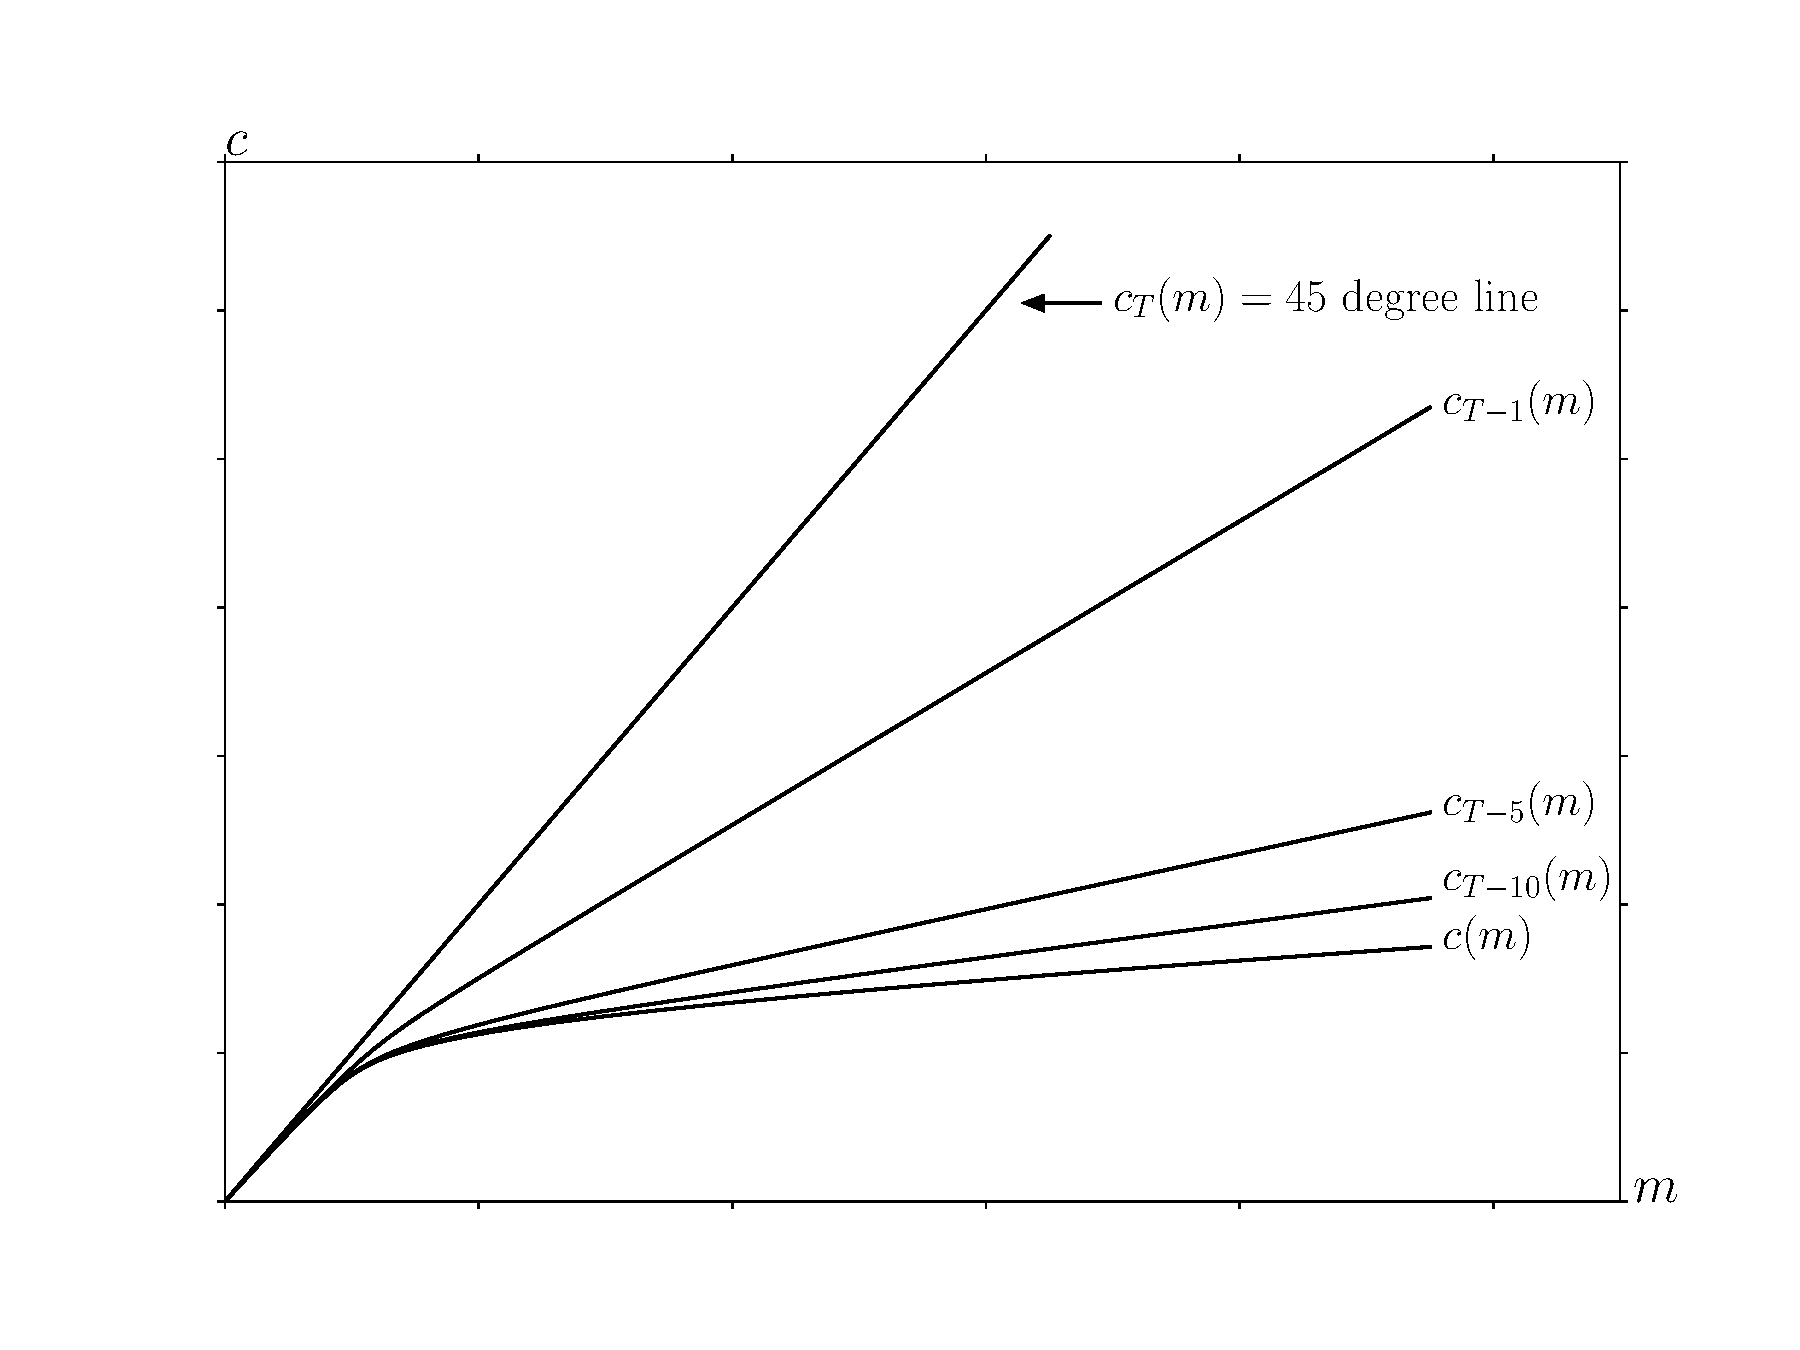
\includegraphics[width=6in]{\FigDir/cFuncsConverge}}
\caption{Convergence of the Consumption Rules}
\label{fig:cFuncsConverge}
\end{figure}
 % Read in the tex to generate the figure

\subsection{Concave Consumption Function Characteristics}\label{sec:cExists}

A precondition for the main theorem is that the maximization problem defines a sequence of continuously differentiable strictly increasing strictly concave\footnote{With one obvious exception: $\usual{\cFunc}_{T}(\mNrm)$ is linear (and so only weakly concave).} functions $\{\cFunc_{T},\cFunc_{T-1},\ldots\}$.  The straightforward but tedious proof is relegated to Appendix~\ref{sec:ApndxConcaveCFunc}.  (\cite{ckConcavity} proved concavity but not continuous differentiability, which our theorem will use). For present purposes, the important point is that the income process induces what~\cite{aiyagari:ge} dubbed a `natural borrowing constraint':  $\usual{\cFunc}_{t}(\mNrm) < m$ for all periods $t < T$ because a consumer who spent all available resources would arrive in period $t+1$ with balances $b_{t+1}$ of zero, and then might earn zero income over the remaining horizon, risking the possibility of a requirement to spend zero, yielding negative infinite utility.  To avoid this calamity, the consumer never spends everything.~~\cite{zeldesStochastic} seems to have been the first to argue, based on his numerical results, that the natural borrowing constraint was a quantitatively plausible alternative to `artificial' or `ad hoc' borrowing constraints.\footnote{The same (numerical) point applies for infinite horizon models (calibrated to actual empirical data on household income dynamics); cf.~\cite{carrollBrookings}.}

Strict concavity and continuous differentiability of the consumption function are key elements in many of the arguments below, but are not characteristics of models with `artificial' borrowing constraints (though the analytical convenience of these features is considerable -- see below).

\hypertarget{Bounds-for-the-Consumption-Functions}{}
\subsection{Bounds for the Consumption Functions}\label{subsec:cFuncBounds}

The consumption functions depicted in Figure~\ref{fig:cFuncsConverge} appear to have limiting slopes as $\mNrm \downarrow 0$ and as $\mNrm \uparrow \infty$.  This section confirms that impression and derives those slopes, which will be needed in the contraction mapping proof.\footnote{\cite{benhabibWealth} show that the consumption function becomes linear as wealth approaches infinity in a model with capital income risk and liquidity constraints;~\cite{maTodaRich} show that these results generalize to the limits derived here if capital income is added to the model.}


Assume (as justified above) that a continuously differentiable concave consumption function exists in period $t+1,$ with an origin at $\usual{\cFunc}_{t+1}(0)=0$, a minimal MPC $\MPCmaxmin_{t+1}>0$, and maximal MPC $\MPCmax_{t+1} \leq 1$.  (If $t+1 = T$ these will be $\MPCmaxmin_{T}=\MPCmax_{T}=1$; for earlier periods they will exist by recursion.)

Under our imposed assumption that human wealth is finite, the MPC bound as wealth approaches infinity is easy to understand: As the \textit{proportion} of consumption that will be financed out of human wealth approaches zero, the proportional difference between the solution to the model with uncertainty and the perfect foresight model shrinks to zero.  \hypertarget{MPCnvrsLower}{} In the course of proving this, Appendix~\ref{sec:MPCLimits} provides a recursive expression (used below) for the (inverse of the) limiting MPC as wealth approaches $\infty$:\hypertarget{WRICCondDefn}{}\hypertarget{MPCmax}{}\hypertarget{MPCnvrsUpperDefn}{}\hypertarget{WRIC}{}\hypertarget{WRPFacDefn}{}
\begin{align}
  \MPCmin_{t}^{-1}  & = 1+\MPSmax \MPCmin_{t+1}^{-1} \label{eq:MPCminInv}.
\end{align}
\subsubsection{The Weak RIC Condition ({WRIC})}{}\label{sec:WRIC}
Appendix equation~\eqref{eq:MPCmaxInvApndx} reflects the derivation of a parallel expression for the limiting maximal MPC as $\mNrm_{t} \downarrow 0$:
\begin{align}
  \MPCmax_{t}^{-1}  & = 1+\MPSmin \MPCmax_{t+1}^{-1} \label{eq:MPCmaxInv}
\end{align}
where $\left\{\MPCmax_{T-n}^{-1}\right\} _{n=0}^{\infty}$ is a decreasing convergent sequence if the `weak return patience factor' $\pZero^{1/\CRRA}\RPFac$ satisfies:
\begin{align}
  \text{{\WRIC}:~~}  1 \geq &~\pZero^{1/\CRRA} \RPFac, \phantom{\text{{\WRIC}:~~}} \label{eq:WRIC}
\end{align}
a condition we dub the `Weak Return Impatience Condition' because with $\pZero < 1$ it will hold more easily (for a larger set of parameter values) than the \RIC~($\RPFac < 1$).  The essence of the argument is that as wealth approaches zero, the overriding consideration that limits consumption is the (recursive) fear of the zero-income events.  (That is why the probability of the zero income event $\pZero$ appears in the expression.)

\hypertarget{cBounds}{}
We are now in position to observe that the optimal consumption function must satisfy
\begin{align}
  \MPCminmin_{t} \mNrm_{t} ~ \leq & ~  \usual{\cFunc}_{t}(\mNrm_{t})  \leq  ~ \MPCmax_{t} \mNrm_{t} \label{eq:cBounds}
\end{align}
because consumption starts at zero and is continuously differentiable, is strictly concave,\footnote{\cite{ckConcavity}} and always exhibits a slope between $\MPCminmin_{t}$ and $\MPCmax_{t}$ (formal proof: Appendix~\ref{sec:Tcomplete}).

\hypertarget{Conditions-Under-Which-the-Problem-Defines-a-Contraction-Mapping}{}
\subsection{The Problem Is a Contraction Mapping Under {WRIC} and {FVAC}}\label{subsec:contraction}

As mentioned above, standard theorems in the contraction mapping literature before and after Stokey et.\ al.~\citeyearpar{slpMethods} require utility or marginal utility to be bounded over the space of possible values of $\mNrm$; that requirement does not apply here because the possibility (however unlikely) of an unbroken string of zero-income events through the end of the horizon means that utility (and marginal utility) are unbounded as $\mNrm \downarrow 0$.  Although a recent literature examines the existence and uniqueness of solutions to Bellman equations in the presence of `unbounded returns' (see, e.g., \cite{mnUnique}), it appears that the techniques in that literature cannot be used to solve the problem here because the required conditions are violated by a problem that incorporates permanent shocks.\footnote{See~\cite{yaoNote} for a detailed discussion of the reasons the existing literature up through~\cite{mnUnique} cannot handle the problem described here.}

Fortunately, Boyd~\citeyearpar{jboydWeighted} provided a weighted contraction mapping theorem that~\cite{asHomogeneous} showed could be used to address the homogeneous case (of which CRRA is an example) in a deterministic framework; later,~\cite{duranDiscounting} showed how to extend the~\cite{jboydWeighted} approach to the stochastic case.
\begin{definition}
  Consider any function $\bullet\in \mathcal{C}(\mathscr{A},\mathscr{B})$ where $\mathcal{C}(\mathscr{A},\mathscr{B})$ is the space of continuous functions from $\mathscr{A}$ to $%
  \mathscr{B}$. Suppose $\boundFunc \in \mathcal{C}(\mathscr{A},\mathscr{B})$ with $%
  \mathscr{B}\subseteq\mathbb{R}$ and $\boundFunc >0$. Then $\bullet$ is $\boundFunc$-bounded if the $\boundFunc$-norm of $\bullet$,
  \begin{equation}
    \Vert \bullet\Vert _{\boundFunc }=\sup_{\mNrm}\left[ \frac{|\bullet(\mNrm)|}{\boundFunc (\mNrm)}\right] ,
    \label{eq:phinorm}
  \end{equation}%
  is finite.
\end{definition}

For $\mathcal{C}_{\boundFunc}\left( \mathscr{A},\mathscr{B}\right) $ defined as the set of functions in $\mathcal{C}(\mathscr{A},\mathscr{B})$ that are $\boundFunc$-bounded; $\wFunc$, $\xFunc$, $\yFunc$, and $\zFunc$ as examples of $\boundFunc$-bounded functions; and using {$\mathbf{0}(\mNrm)=0$} to indicate the function that returns zero for any argument, Boyd~\citeyearpar{jboydWeighted} proves the following.

\textbf{Boyd's Weighted Contraction Mapping Theorem.} \textit{Let $\BoydT:\mathcal{C}_{\boundFunc }\left( \mathscr{A},\mathscr{B}\right)
  \rightarrow \mathcal{C}\left( \mathscr{A},\mathscr{B}\right) $ such
  that}\footnote{We will usually denote the function that results from the mapping as, e.g., $\{\BoydT\wFunc\}$.}\textsuperscript{,}\footnote{To non-theorists, this notation may be slightly confusing; the inequality relations in (1) and (3) are taken to mean `for any specific element $\bullet$ in the domain of the functions in question' so that, e.g., $\xFunc \leq \yFunc$ is short for $\xFunc(\bullet) \leq \yFunc(\bullet)~\forall~\bullet\in \mathscr{A}$.  In this notation, $\zeta \Shrinker \boundFunc$ in (3) is a \textit{function} which can be applied to any argument $\bullet$ (because $\boundFunc$ is a function).} \nopagebreak
\begin{align*}
  \mbox{(1)} &\BoydT%
               \mbox{ \textit{is non-decreasing, i.e.\ ${\xFunc} \leq {\yFunc}\Rightarrow
               \{\BoydT{\xFunc}\} \leq \{\BoydT{\yFunc}\}$}}   \nonumber \\
  \mbox{(2)} & \{\BoydT\mathbf{0}\}\in ~ \mathcal{C}_{\boundFunc }\left(\mathscr{A},\mathscr{B}\right)  \notag \\
  \mbox{(3)}
             & \mbox{\textit{There exists some real $0 < \Shrinker < 1$ such that}} \\
             & \{\BoydT({\wFunc} +\zeta\boundFunc )\} \leq \{\BoydT{\wFunc}\} +\zeta\Shrinker \boundFunc
               \mbox{ \textit{~~holds for all real $\zeta > 0$ } } .
\end{align*}
\textit{Then $\BoydT$ defines a contraction with a unique fixed point.}

For our problem, take $\mathscr{A}$ as $\mathbb{R}_{>0}$ and $\mathscr{B}$
as $\mathbb{R}$, and define
\begin{align*}
  \{\EEndMap \zFunc\}(a_{t})  & = \Ex_{t}\left[\PermGroFac^{1-\CRRA}_{t+1} \zFunc(a_{t} \RNrm_{t+1} + \TranShkAll_{t+1})\right].
\end{align*}

Using this, we introduce the mapping \textit{$\TMap:\mathcal{C}_{\boundFunc }\left( \mathscr{A},\mathscr{B}\right) \rightarrow \mathcal{C}\left( \mathscr{A},\mathscr{B}\right) $}.\footnote{Note that the existence of the maximum is assured by the continuity of $\{\EEndMap \zFunc\}(a_{t})$ (it is continuous because it is the sum of continuous $\boundFunc$-bounded functions $\zFunc$) and the compactness of $[\MPCminmin \mNrm_{t}, \MPCmax \mNrm_{t}]$.}\hypertarget{Contraction-Conditions}{}
Our operator $\TMap$ satisfies the conditions that Boyd requires of his operator $\BoydT$ if we impose two restrictions on parameter values.\footnote{See the appendix.}  The first is the \WRIC~necessary for convergence of the maximal MPC, equation~\eqref{eq:WRIC} above.  More serious is the Finite Value of Autarky Condition, equation~\eqref{eq:FVAC}.  (The interpretation of these restrictions is elaborated in Section~\ref{sec:discussConvergence} below.)  Imposing these restrictions, we are now in position to state the central theorem of the paper.

\hypertarget{MainTheorem}{}
\setcounter{theorem}{0}
\begin{theorem}\label{thm:contmap}
  $\TMap$ is a contraction mapping if the weak return impatience condition \eqref{eq:WRIC} and the finite value of autarky condition \eqref{eq:FVAC} hold.
\end{theorem}

Intuitively, Boyd's theorem shows that if you can find a $\boundFunc$ that is everywhere finite but goes to infinity `as fast or faster' than the function you are normalizing with $\boundFunc$, the normalized problem defines a contraction mapping.  The intuition for the {\FVAC} condition is that, with an infinite horizon, with any strictly positive initial amount of bank balances $\bNrm_{0}$, in the limit your value can always be made greater than you would get by consuming exactly the sustainable amount (say, by consuming $(\rfree/\Rfree)\bNrm_{0}-\epsilon$ for some arbitrarily small $\epsilon>0$).

We use the bounding function
\begin{verbatimwrite}{\EqDir/boundFunc}
\begin{equation}\begin{gathered}\begin{aligned}
      \iflabelexists{eq:boundFunc}{}{\label{eq:boundFunc}} % Don't define it if already defined
      \boundFunc(\mNrm)  & = \eta + \mNrm^{1-\CRRA},
    \end{aligned}\end{gathered}\end{equation}
\end{verbatimwrite}
\begin{equation}\begin{gathered}\begin{aligned}
      \iflabelexists{eq:boundFunc}{}{\label{eq:boundFunc}} % Don't define it if already defined
      \boundFunc(\mNrm)  & = \eta + \mNrm^{1-\CRRA},
    \end{aligned}\end{gathered}\end{equation}

for some real scalar $\eta > 0$ whose value is determined in the course of the proof.\footnote{Thanks to John Boyd for suggesting this bounding function.} Under this definition of $\boundFunc$, $\{\TMap\mathbf{0}\}(\mNrm_{t})= \uFunc(\MPCmax \mNrm_{t})$ is clearly $\boundFunc$-bounded.  

The cumbersome details of the proof are relegated to Appendix~\ref{sec:Tcomplete}.  Given that the value function converges, Appendix~\ref{subsec:cConverges} shows that the consumption functions converge.\footnote{MST's proof is for convergence of the consumption policy function directly, rather than of the value function, which is why their conditions are on $\uFunc^{\prime}$, which governs behavior.}

\hypertarget{The-Liquidity-Constrained-Solution-as-a-Limit}{}
\subsection{The Liquidity Constrained Solution as a Limit}\label{sec:deatonIsLimit}

This section explains why a related problem commonly considered in the literature (e.g., by Deaton~\citeyearpar{deatonLiqConstr}), with a liquidity constraint and a positive minimum value of income, is the limit of the problem considered here as the probability $\pZero$ of the zero-income event approaches zero.

The `related' problem makes two changes to the problem defined above:
\begin{enumerate}
\item An `artificial' liquidity constraint is imposed: $\aNrm_{t}\geq 0$
\item The probability of zero-income events is zero: $\pZero=0$
\end{enumerate}

The essence of the argument is simple.  Imposing the artificial constraint without changing $\pZero$ would not change behavior at all: The possibility of earning zero income over the remaining horizon already prevents the consumer from ending the period with zero assets.  So, for precautionary reasons, the consumer will save something.

But the \textit{extent} to which the consumer feels the need to make this precautionary provision depends on the \textit{probability} that it will turn out to matter.  As $\pZero \downarrow 0$, that probability becomes arbitrarily small, so the \textit{amount} of precautionary saving induced by the zero-income events approaches zero as $\pZero \downarrow 0$.  But ``zero'' is the amount of precautionary saving that would be induced by a zero-probability event for the impatient liquidity constrained consumer.

Another way to understand this is just to think of the liquidity constraint reflecting a component of the utility function that is zero whenever the consumer ends the period with (strictly) positive assets, but negative infinity if the consumer ends the period with (weakly) negative assets.



\hypertarget{Factors-Defined-And-Compared}{}
  \begin{table}[!th]
    \centering
\caption{Definitions and Comparisons of Conditions}
  \iflabelexists{table:Comparison}{}{\label{table:Comparison}} % Don't define it if already defined
  \sbox{\TblBox}{
\begin{tabular}{|c|c|}\hline
Perfect Foresight Versions & Uncertainty Versions\\ \hline
\multicolumn{2}{|c|}{Finite Human Wealth Condition (\FHWC)} \\ \hline
$\PermGroFac/\Rfree < 1$                                                          & $\PermGroFac/\Rfree < 1$ \\
\multirow{3}{75mm}{\thead{The growth factor for permanent income \\ $\PermGroFac$ must be smaller than the discounting \\ factor $\Rfree$ for human wealth to be finite. }} &
\multirow{3}{75mm}{\thead{The model's risks are mean-preserving \\ spreads, so the PDV of future income is \\ unchanged by their introduction.}} \\
&  \\
&  \\
&  \\ \hline
\multicolumn{2}{|c|}{Absolute Impatience Condition (\AIC)} \\ \hline
$\APFac < 1$                                        &  $\APFac < 1$ \\
\multirow{4}{75mm}{\thead{The unconstrained consumer is \\ sufficiently impatient that the level of \\ consumption will be declining over time:}} &
\multirow{4}{75mm}{\thead{\textit{If wealth is large enough,} the \textit{expectation} \\ of consumption next period will be \\ smaller than this period's consumption:}} \\
& \\
& \\
& \\
$\cLvl_{t+1} < \cLvl_{t}$ & $\lim_{m_{t} \rightarrow \infty} \Ex_{t} [\cLvl_{t+1}] < \cLvl_{t}$ \\
& \\ \hline
\multicolumn{2}{|c|}{Return Impatience Conditions} \\ \hline
\multicolumn{1}{|c|}{Return Impatience Condition (\RIC)} & \multicolumn{1}{c|}{Weak \RIC~(\WRIC)} \\ \hline
$\APFac/\Rfree < 1$                                          & $\pZero^{1/\CRRA}\APFac/\Rfree < 1$ \\
\multirow{3}{75mm}{\thead{The growth factor for consumption $\APFac$ \\ must be smaller than the discounting \\ factor $\Rfree$, so that the PDV of current and \\ future consumption will be finite:}}  &
\multirow{3}{75mm}{\thead{If the probability of the zero-income \\ event is $\pZero=1$ then income is always zero \\ and the condition becomes identical to \\ the \RIC.  Otherwise, weaker.}} \\
& \\
& \\
& \\
& \\
$\cFunc^{\prime}(m) = 1-\APFac/\Rfree < 1$              & $\cFunc^{\prime}(m) < 1-\pZero^{1/\CRRA}\APFac/\Rfree < 1$ \\
& \\ \hline
\multicolumn{2}{|c|}{Growth Impatience Conditions} \\ \hline
\multicolumn{1}{|c|}{\GICRaw} & \multicolumn{1}{c|}{\GICNrm} \\ \hline
$\APFac/\PermGroFac < 1$                                         & $\APFac\Ex[\PermShk^{-1}]/\PermGroFac < 1 $ \\
\multirow{4}{75mm}{\thead{For an unconstrained PF consumer, the \\ ratio of $\cLvl$ to $\PermLvl$ will fall over time.  For \\ constrained, guarantees the constraint \\ eventually binds. Guarantees \\ ~~~~~~$\lim_{\mNrm_{t}\uparrow\infty} \Ex_{t}[\PermShk_{t+1}\mNrm_{t+1}/\mNrm_{t}] = \GPFacRaw$}} &
\multirow{4}{75mm}{\thead{By Jensen's inequality stronger than \GICRaw.\\  Ensures consumers will not expect to \\ accumulate $\mNrm$ unboundedly.}} \\
& \\
& \\
& \\
& $\lim_{\mNrm_{t} \rightarrow \infty} \Ex_{t}[\mNrm_{t+1}/\mNrm_{t}] = \GPFacNrm $
 \\
&  \\ \hline
\multicolumn{2}{|c|}{Finite Value of Autarky Conditions} \\ \hline
\multicolumn{1}{|c|}{\PFFVAC} & \multicolumn{1}{c|}{\FVAC} \\ \hline
$\beta \PermGroFac^{1-\CRRA} < 1$                                                 & $\beta \PermGroFac^{1-\CRRA}\Ex[\PermShk^{1-\CRRA}] < 1$  \\
equivalently $\APFac  < \Rfree^{1/\CRRA}\PermGroFac^{1-1/\CRRA}$ & \\
\multirow{3}{75mm}{\thead{The discounted utility of constrained \\ consumers who spend their permanent \\ income each period should be finite.}} &
\multirow{3}{75mm}{\thead{By Jensen's inequality, stronger than the \\ \PFFVAC~because for $\CRRA>1$ and \\ nondegenerate $\PermShk$, $\Ex[\PermShk^{1-\CRRA}] > 1$.} } \\
& \\
                           & \\
&  \\ \hline
\end{tabular}
} % End \sbox

    \settowidth\TableWidth{\usebox{\TblBox}}
    \savebox{\TblShrunkBox}{
      \settowidth{\TblShrunk}{\usebox{\TblBox}}
      \resizebox{0.9\textwidth}{!}{\begin{minipage}{\TblShrunk}
          \usebox{\TblBox}
        \end{minipage}}
    }

    \usebox{\TblShrunkBox}

\end{table}


See Appendix~\ref{sec:LiqConstrAsLimit} for the formal proof justifying the foregoing intuitive discussion.\footnote{It seems likely that a similar argument would apply even in the context of a model like that of MST, perhaps with some weak restrictions on returns.}

The conditions required for convergence and nondegeneracy are thus strikingly similar between the liquidity constrained perfect foresight model and the model with uncertainty but no explicit constraints: The liquidity constrained perfect foresight model is just the limiting case of the model with uncertainty as the degree of all three kinds of uncertainty (zero-income events, other transitory shocks, and permanent shocks) approaches zero.

% \hypertarget{Restrained-Consumer}{}
% In the remainder of the paper, in order to avoid a confusion that is common in discussions of models of this type, we will refer to consumers who are solving a problem in which constraints exist, but are not necessarily binding at the moment under consideration, as `restrained' consumers.


\hypertarget{Relations-Between-Parametric-Restrictions}{}
\subsection{Relations Between Parametric Restrictions}\label{sec:discussConvergence}

The full relationship among conditions is represented in Figure~\ref{fig:Inequalities}.  Though the diagram looks complex, it is merely a modified version of the earlier simple diagram (Figure~\ref{fig:RelatePFGICFHWCRICPFFVAC}) with further (mostly intermediate) inequalities inserted.  (Arrows with a ``because'' now label relations that always hold under the model's assumptions.)\footnote{Again, readers unfamiliar with such diagrams should see Appendix~\ref{sec:ApndxConditionDiagrams} for a more detailed exposition.}

\renewcommand{\figName}{Inequalities} 
\renewcommand{\figFile}{\figName} 
\hypertarget{\figFile}{}
\input{\FigDir/\figName} % Read in the tex to generate the figure

% \subsubsection{The \WRIC}\label{subsubsec:WRICdiscuss}

The `weakness' of the additional condition sufficient for contraction beyond the {\FVAC}, the \WRIC, can be seen by asking `under what circumstances would the \FVAC~hold but the \WRIC~fail?'  Algebraically, the requirement is
\begin{align}
  \DiscFac \PermGroFac^{1-\CRRA}\uInvEuPermShk^{1-\CRRA} & < ~ 1 ~ <  {(\pZero \DiscFac)}^{1/\CRRA}/\Rfree^{1-1/\CRRA}. \label{eq:WRICandFVAC}
\end{align}

If we require $\Rfree \geq 1$, the {\WRIC}~is redundant because now $\DiscFac <1<\Rfree^{\CRRA-1}$, so that (with $\CRRA > 1$ and $\DiscFac<1$) the \RIC~(and \WRIC) must hold.  But neither theory nor evidence demand that $\Rfree \geq 1$.  We can therefore approach the question of the \WRIC's relevance by asking just how low $\Rfree$ must be for the condition to be relevant.  Suppose for illustration that $\CRRA=2$, $\uInvEuPermShk^{1-\CRRA}=1.01$, $\PermGroFac^{1-\CRRA}=1.01^{-1}$ and $\pZero = 0.10$.  In that case~\eqref{eq:WRICandFVAC} reduces to
\begin{align*}
  \DiscFac  & < 1 < {(0.1 \DiscFac/\Rfree)}^{1/2}
\end{align*}
but since $\DiscFac < 1$ by assumption, the binding requirement is that
\begin{align*}
  \Rfree  & < \DiscFac/10 \notag
\end{align*}
so that for example if $\DiscFac=0.96$ we would need $\Rfree < 0.096$ (that is, a perpetual riskfree rate of return of worse than -90 percent a year) in order for the \WRIC~to bind. 


Perhaps the best way of thinking about this is to note that the space of parameter values for which the \WRIC~is relevant shrinks out of existence as $\pZero \rightarrow 0$, which Section~\ref{sec:deatonIsLimit} showed was the precise limiting condition under which behavior becomes arbitrarily close to the liquidity constrained solution (in the absence of other risks).  On the other hand, when $\pZero = 1$, the consumer has no noncapital income (so that the \FHWC~holds) and with $\pZero=1$ the \WRIC~is identical to the RIC;\@ but the \RIC~is the only condition required for a solution to exist for a perfect foresight consumer with no noncapital income.  Thus the WRIC~forms a sort of `bridge' between the liquidity constrained and the unconstrained problems as $\pZero$ moves from 0 to 1.



\hypertarget{IntuitionRIC}{}
\subsubsection{When the {RIC}~Fails}\label{subsubsec:WhenTheRICFails}



In the perfect foresight problem (Section~\ref{subsec:PFUncon}), the \RIC~was necessary for existence of a nondegenerate solution.  It is surprising, therefore, that in the presence of uncertainty, the much weaker {\WRIC} is sufficient for nondegeneracy (assuming that the {\FVAC} holds).  We can directly derive the features the problem must exhibit (given the \FVAC) under \cncl{\RIC} (that is, $\Rfree < {(\Rfree \DiscFac)}^{1/\CRRA})$:
\begin{equation}\label{eq:RICimplies}
  \begin{split}
    \Rfree   & < \overbrace{{(\Rfree \DiscFac)}^{1/\CRRA} ~ < ~ {(\Rfree {(\PermGroFac \uInvEuPermShk)}^{\CRRA-1})}^{1/\CRRA}}^{\text{implied by \FVAC}}
    \\  \Rfree   & < {(\Rfree/\PermGroFac)}^{1/\CRRA}\PermGroFac \uInvEuPermShk^{1-1/\CRRA}
                   %         \\  \Rfree/\PermGroFac  & < {(\Rfree/\PermGroFac)}^{1/\CRRA}\uInvEuPermShk^{1-1/\CRRA}
    \\  \Rfree/\PermGroFac  & < \uInvEuPermShk
  \end{split}
\end{equation}
but since $\uInvEuPermShk < 1$ (cf.\ the argument below~\eqref{eq:uInvEuPermShk}), this requires $\Rfree/\PermGroFac < 1$; so, given the \FVAC, the \RIC~can fail only if human wealth is unbounded.  As an illustration of the convenience of our diagrams, note that this algebraically complicated conclusion could be easily reached diagrammatically in figure~\ref{fig:Inequalities} by starting at the $\Rfree$ node and imposing $\cncl{\RIC}$, which reverses the {\RIC} arrow and lets us traverse the diagram along any clockwise path to the {\PFVAFacDefn} node at which point we realize that we \textit{cannot} impose the {\FHWC} because that would let us conclude $\Rfree > \Rfree$.

As in the perfect foresight constrained problem, unbounded limiting human wealth (\cncl{\FHWC}) here does not lead to a degenerate limiting consumption function (finite human wealth is not required for the convergence theorem).  But, from equation~\eqref{eq:MPCminInv} and the discussion surrounding it, an implication of \cncl{\RIC} is that $\lim_{m \uparrow \infty} \usual{\cFunc}^{\prime}(\mNrm) = 0$.  Thus, interestingly, in the special $\{\cncl{\RIC},~\cncl{\FHWC}\}$ case (unavailable in the perfect foresight model) the presence of uncertainty both permits unlimited human wealth (in the $n\uparrow\infty$ limit) and at the same time prevents unlimited human wealth from resulting in (limiting) infinite consumption (at any finite $\mNrm$).  Intuitively, in the presence of uncertainty, pathological patience (which in the perfect foresight model results in a limiting consumption function of $\usual{\cFunc}(\mNrm)=0$) plus unbounded human wealth (which the perfect foresight model prohibits because it leads to a limiting consumption function $\usual{\cFunc}(\mNrm)=\infty$ for any finite $\mNrm$) combine to yield a unique finite limiting (as $n \uparrow \infty$) level of consumption and MPC for any finite value of $\mNrm$.  Note the close parallel to the conclusion in the perfect foresight liquidity constrained model in the \{\GICRaw,~\cncl{\RIC}\} case.  There, too, the tension between infinite human wealth and pathological patience was resolved with a nondegenerate consumption function whose limiting MPC was zero.\footnote{\cite{maTodaRich} derive conditions under which the limiting MPC is zero in an even more general case where there is also capital income risk.}

\hypertarget{When-the-RIC-Holds}{}
\subsubsection{When the {RIC} Holds}\label{subsubsec:WhenTheGICModFails}\label{subsubsec:WhenTheRICHolds}

\textbf{\FHWC}.  If the {\RIC} and {\FHWC} both hold, a perfect foresight solution exists (see~\ref{subsec:PFUncon} above).  As $\mNrm \uparrow \infty$ the limiting $\cFunc$ and $\vFunc$ functions become arbitrarily close to those in the perfect foresight model, because human wealth pays for a vanishingly small portion of spending.  This will be the main case analyzed in detail below.

\noindent \textbf{\cncl{\FHWC}}.  The more exotic case is where {\FHWC} fails; in the perfect foresight model, \{{\RIC},\cncl{\FHWC}\} is the degenerate case with limiting $\bar{\cFunc}(\mNrm)=\infty$.  Here, the {\FVAC} implies that the {\PFFVAC} holds (traverse Figure~\ref{fig:Inequalities} clockwise from $\APFac$ by imposing {\FVAC} and continue to the {\PFVAFacDefn} node):  Reversing the arrow connecting the $\Rfree$ and {\PFVAFacDefn} nodes implies that under $\cncl{\FHWC}$:
\begin{align*}
  & \overbrace{\APFac < {(\Rfree/\PermGroFac)}^{1/\CRRA}\PermGroFac}^{\PFFVAC}
  \\ & \APFac < \PermGroFac
\end{align*}
where the transition from the first to the second lines is justified because $\cncl{\FHWC} \Rightarrow {(\Rfree/\PermGroFac)}^{1/\CRRA}<1$.  So, \{\RIC, \cncl{\FHWC}\} implies the {\GICRaw} holds.  However, we are not entitled to conclude that the {\GICMod} holds: $\APFac < \PermGroFac$ does not imply $\APFac < \InvEPermShkInv \PermGroFac$ where $\InvEPermShkInv<1$.  

We have now established the principal points of comparison between the perfect foresight solutions and the solutions under uncertainty; these are codified in the remaining parts of Tables~\ref{table:Comparison} and~\ref{table:Required}.

\hypertarget{Sufficient-Conditions}{}
\hypertarget{Sufficient-Conditions-For-Nondegenerate-Solution}{}

\newsavebox{\Required}
\begin{table}
\centering
\caption{Sufficient Conditions for Nondegenerate$^{\ddagger}$ Solution}
  \iflabelexists{table:Required}{}{\label{table:Required}} % Don't define it if already defined
\sbox{\Required}{
\begin{tabular}{|l|l|l|} \hline
  \multicolumn{1}{|l|}{Consumption Model(s)}                                                                             & \multicolumn{1}{c|}{Conditions}         & \multicolumn{1}{c|}{Comments}
%    \\\multicolumn{1}{|r|}{ Reference            }                                                                         &                                         & \multicolumn{1}{c|}{Logic}
    \\ \hline
        \multicolumn{1}{|l|}{$\bar{\cFunc}(m)$: PF Unconstrained}                                                              & \RIC, \FHWC$^{\circ}$                   & \RIC$\Rightarrow |\vFunc(\mNrm)|< \infty$; \FHWC$ \Rightarrow 0 < |\vFunc(\mNrm)|$
    \\ {$\underline{\cFunc}(m)=\MinMPC \mNrm$}                                                                &                                         & PF model with no human wealth ($h=0$)
    \\\multicolumn{1}{|l|}{}                                                                         &                                          \multicolumn{1}{c|}{} &                                          \multicolumn{1}{c|}{}
    \\ \multicolumn{1}{|r|}{\href{https://\owner.github.io/BufferStockTheory\#PF-Unconstrained-Solution}{Section \ref{subsec:PFUncon}:}}         &                                         & \RIC prevents $\bar{\cFunc}(\mNrm)=\underline{\cFunc}(\mNrm)=0$
    \\ \multicolumn{1}{|r|}{\href{https://\owner.github.io/BufferStockTheory\#PF-Unconstrained-Solution}{Section \ref{subsec:PFUncon}:}}         &                                         & {\FHWC} prevents $\bar{\cFunc}(\mNrm)=\infty$
    \\ \multicolumn{1}{|r|}{Eq \eqref{eq:FHWCandPFFVACimplyRIC}:}                                                                              &                                         & {\PFFVAC}+{\FHWC} $\Rightarrow$ {\RIC}
    \\ \multicolumn{1}{|r|}{{Eq \eqref{eq:GICandFHWCimplyPFFVAC}}:}                                                                              &                                         & {\GICRaw}+{\FHWC} $\Rightarrow$ {\PFFVAC}
    \\ \hline\hline \multicolumn{1}{|l|}{$\cnstr{\cFunc}(m)$: PF Constrained}                                              & \cncl{\GICRaw}, \RIC                    & {\FHWC} holds $(\PGro < \Pat < \Rfree \Rightarrow \PGro < \Rfree)$
    \\
\multicolumn{1}{|r|}{\href{https://\owner.github.io/BufferStockTheory\#PF-Constrained-Solution}{Section \ref{subsec:PFCon}:}}                &                                         & $\cnstr{\cFunc}(\mNrm)=\bar{\cFunc}(\mNrm)$ for $\mNrm > \mNrm_{\#} < 1$
    \\                                                                                                                        &                                         & (\cncl{\RIC} would yield $\mNrm_{\#}=0$ so $\cnstr{\cFunc}(\mNrm)=0$)
%  \\ \cline{2-3} \href{https://\owner.github.io/BufferStockTheory\#ApndxLiqConstr}{Appendix \ref{sec:ApndxLiqConstr}} & \GICRaw,\RIC                            & $\lim_{\mNrm \rightarrow \infty} \cnstr{\cNrm}(\mNrm)=\bar{\cNrm}(\mNrm), \lim_{\mNrm \rightarrow \infty} \cnstr{\MPCFunc}(\mNrm)=\MinMPC$
    \\ \cline{2-3}  \multicolumn{1}{|r|}{\href{https://\owner.github.io/BufferStockTheory\#ApndxLiqConstr}{Appendix \ref{sec:ApndxLiqConstr}}:} & \GICRaw,\RIC                            & $\lim_{\mNrm \rightarrow \infty} \cnstr{\cNrm}(\mNrm)=\bar{\cNrm}(\mNrm), \lim_{\mNrm \rightarrow \infty} \cnstr{\MPCFunc}(\mNrm)=\MinMPC$
    \\                                                                                                                        &                                         & kinks where horizon to $b=0$ changes$^{\ast}$
    \\ \cline{2-3}\multicolumn{1}{|r|}{\href{https://\owner.github.io/BufferStockTheory\#ApndxLiqConstr}{Appendix \ref{sec:ApndxLiqConstr}}:}  & \GICRaw,\cncl{\RIC}                     & $\lim_{\mNrm \rightarrow \infty}  \cnstr{\MPCFunc}(\mNrm)=0$
    \\                                                                                                                        &                                         & kinks where horizon to $b=0$ changes$^{\ast}$
    \\ \hline\hline \multicolumn{1}{|l|}{$\usual{\cFunc}(\mNrm)$:  \href{https://\owner.github.io/BufferStockTheory\#Uncertainty-Modified-Conditions}{Friedman/Muth}
  }                                                                                                                       & Section \ref{subsec:LimitsAsmtToInfty}, & $\underline{\cFunc}(\mNrm) < \usual{\cFunc}(\mNrm) < \bar{\cFunc}(\mNrm)$ %\phantom{\RIC, \FHWC$^{\ast\ast}$  }
    \\                                                                                                                      & Section \ref{subsec:LimitsAsmtToZero}   & $\underline{\vFunc}(\mNrm) < \usual{\vFunc}(\mNrm) < \bar{\vFunc}(\mNrm)$ %
  % \\ \hline\hline \multicolumn{1}{|l|}{$\usual{\cFunc}(\mNrm)$: Friedman/Muth}                                          & \FVAC, \WRIC                            & \WRIC is weaker than \RIC
%   \\ {``Buffer Stock'' Subset}                                                                                       &                                         & \GICNrm $\Rightarrow \exists $ `individual target' $\mTrgNrm$
%   \\ { Section \ref{subsec:onetarget}}                                                                             &                                         & \GICRaw $\Rightarrow \exists $ `individual steady-state' $\mBalLvl$

  \\ \cline{2-3}\multicolumn{1}{|r|}{Section \ref{subsec:contraction}:}                            & \FVAC, \WRIC                      & Sufficient for Contraction
 \\ \multicolumn{1}{|r|}{Section \ref{sec:discussConvergence}:}                               &                      & \WRIC is weaker than \RIC
\\  \multicolumn{1}{|r|}{Figure \ref{fig:Inequalities}:}                                        &                                 & \FVAC is stronger than \PFFVAC
  \\ \multicolumn{1}{|r|}{Section \ref{subsubsec:WhenTheRICHolds}:}
                                            &                                 & \cncl{\FHWC}+RIC $\Rightarrow $\GICRaw$, \lim_{\mNrm \rightarrow \infty} \usual{\MPCFunc}(\mNrm)=\MinMPC$
  \\  \multicolumn{1}{|r|}{Section \ref{subsubsec:WhenTheRICFails}:}                                        &                                 & \cncl{\RIC}  $\Rightarrow $\cncl{\FHWC}$, \lim_{\mNrm \rightarrow \infty} \usual{\MPCFunc}(\mNrm)=0$
  \\ \cline{3-3}\multicolumn{1}{|r|}{Section \ref{subsec:onetarget}:}                                        &                                 & ``Buffer Stock Saving'' Conditions
  \\ \multicolumn{1}{|r|}{Section \ref{subsubsec:mSteadyState}:}                                        &                                 & \phantom{-Nrm}{\GICRaw} $\Rightarrow \exists 0 < \mBalLvl < \infty$ %: Steady-State
  \\ \multicolumn{1}{|r|}{Section \ref{subsubsec:mTarget}:}                                        &                                 & {\GICNrm} $\Rightarrow \exists 0 < \mTrgNrm < \infty$ %: Target
%  \\ \hline\hline \multicolumn{1}{|l|}{$\usual{\cFunc}(\mNrm)$: Friedman/Muth} & \RIC, \FHWC                      & $\underline{\cFunc}(\mNrm) < \usual{\cFunc}(\mNrm) < \bar{\cFunc}(\mNrm)$
%  \\ {``Buffer Stock'' Subset}                                         &                                 & \GICNrm $\Rightarrow \exists $ `individual target' $\mTrgNrm$
%\\ { Section \ref{subsec:onetarget}}                                         &                                 & \GICRaw~$\Rightarrow \exists $ `individual steady-state' $\mBalLvl$

\\ \hline \multicolumn{3}{c}{}
\end{tabular}
} % End \sbox

\settowidth\TableWidth{\usebox{\Required}}
%\usebox{\Required}
\newlength{\RequiredShrunk}
\newsavebox{\RequiredShrunkBox}

\savebox{\RequiredShrunkBox}{
  \settowidth{\RequiredShrunk}{\usebox{\Required}}
  \resizebox{\textwidth}{!}{\begin{minipage}{\RequiredShrunk}
      \usebox{\Required}
    \end{minipage}}
}

\usebox{\RequiredShrunkBox}


\parbox{\textwidth}{\footnotesize         $^{\ddagger}$For feasible $\mNrm$ satisfying $0 < \mNrm < \infty$, a nondegenerate limiting consumption function defines a unique optimal value of $\cNrm$ satisfying $0 < \cNrm(m) < \infty$; a nondegenerate limiting value function defines a corresponding unique value of $-\infty < \vFunc(\mNrm) < 0$ .\\
  ~~$^{\circ}$RIC, \FHWC~are necessary as well as sufficient for the perfect foresight case.~~$^{\ast}$That is, the first kink point in $\cNrm(\mNrm)$ is $\mNrm_{\#}$ s.t. for $\mNrm < \mNrm_{\#}$ the constraint will bind now, while for $\mNrm > \mNrm_{\#}$ the constraint will bind one period in the future.  The second kink point corresponds to the $\mNrm$ where the constraint will bind two periods in the future, etc.\\
  ~~$^{\ast\ast}$In the Friedman/Muth model, the {\RIC}+{\FHWC} are sufficient, but \textit{not} necessary for nondegeneracy}
\end{table}



\hypertarget{AnalysisoftheConvergedConsumptionFunction}{}
\section{Analysis of the Converged Consumption Function}\label{sec:convergedcfunc}

Figures~\ref{fig:cNrmTargetFig}-\ref{fig:cFuncBounds} capture the main properties of the converged consumption rule when the \RIC, \GICMod, and \FHWC~all hold.\footnote{These figures reflect the converged rule corresponding to the parameter values indicated in Table~\ref{table:Calibration}.}

Figure~\ref{fig:cNrmTargetFig} shows the expected growth factors for consumption, the level of market resources, and the market resources ratio, $\Ex_{t}[\cLvl_{t+1}/\cLvl_{t}]$ and $\Ex_{t}[\mLvl_{t+1}/\mLvl_{t}]$, and $\Ex_{t}[\mNrm_{t+1}/\mNrm_{t}]$, for a consumer behaving according to the converged consumption rule, while Figures~\ref{fig:mpclimits}---\ref{fig:cFuncBounds} illustrate theoretical bounds for the consumption function and the MPC.

Three points are worth highlighting.  % features of behavior are captured, or suggested, by the figures.

First, as $\mNrm_{t} \uparrow \infty$ the expected consumption growth factor goes to ${\APFac}$, indicated by the lower bound in Figure~\ref{fig:cNrmTargetFig}, and the marginal propensity to consume approaches $\MPCmin=(1-\RPFac)$ (see Figure~\ref{fig:mpclimits}) --- the same as the perfect foresight MPC.\@  Second, as $\mNrm_{t}$ approaches zero the consumption growth factor approaches $\infty$ (Figure~\ref{fig:cNrmTargetFig}) and the MPC approaches $\MPCmax=(1-\pZero^{1/\CRRA}\RPFac)$ (Figure~\ref{fig:mpclimits}).  Third, there is a value of the market resources ratio $\mNrm_{t} = \mBalLvl$ at which the expected growth rate of the level of market resources $\mLvl$ matches the expected growth rate of permanent income $\PermGroFac$, and a different (larger) target ratio $\mTrgNrm$ where $\Ex[\mNrm_{t+1}/\mNrm_{t}]=1$ (and the expected growth rate of consumption is lower than $\PermGroFac$).  Thus, at the individual level, this model does not have a single $\mNrm$ at which $\PermLvl,~\mLvl,~$ and $\cLvl$ all are expected to grow at the same rate.

\begin{comment}
  Third (Figure~\ref{fig:cNrmTargetFig}), there are two special values of $\mNrm$, which we will call the `individual balanced growth' point $\mBalLvl$ because it is the point where expected consumption growth and expected permanent income growth are balanced, and the `individual target' $\mTrgNrm$ such that if $\mNrm_t = \mTrgNrm$ then $\Ex_t [{\mNrm}_{t+1}] = \mNrm_t$.  %As indicated by the arrows of motion on the $\Ex_{t}[\cLvl_{t+1}/\cLvl_{t}]$ curve, the model's dynamics are `stable' around this target in the sense that if $\mNrm_{t} < \mTrgNrm$ then $\mNrm$ will rise (in expectation), while if $\mNrm_{t} > \mTrgNrm$, it will fall (in expectation).Fourth (Figure~\ref{fig:cNrmTargetFig}), at the market resources target $\mTrgNrm$, the expected rate of growth of consumption is slightly less than the expected growth rate
  of permanent noncapital income.  (The individual consumer does not expect `balanced growth' at $\mTrgNrm$).

  The final proposition suggested by Figure~\ref{fig:cNrmTargetFig} is that the expected consumption growth factor is declining in the level of the cash-on-hand ratio $\mNrm_{t}$.  This turns out to be true in the absence of permanent shocks, but in extreme cases it can be false if permanent shocks are present.\footnote{Throughout the remaining analysis I make a final assumption that is not strictly justified by the foregoing.  We have seen that the finite-horizon consumption functions $\usual{\cFunc}_{T-n}(\mNrm)$ are twice continuously differentiable and strictly concave, and that they converge to a continuous function $\usual{\cFunc}(\mNrm)$.  It does not strictly follow that the limiting function $\usual{\cFunc}(\mNrm)$ is twice continuously differentiable, but I will assume that it is.}
\end{comment}

\renewcommand{\figFile}{cNrmTargetFig}
\hypertarget{\figFile}{}
% Could not get fonts to work right for svg version of this figure for web; so use png
\ifthenelse{\boolean{Web}}{
\begin{figure}[tbp]
\centerline{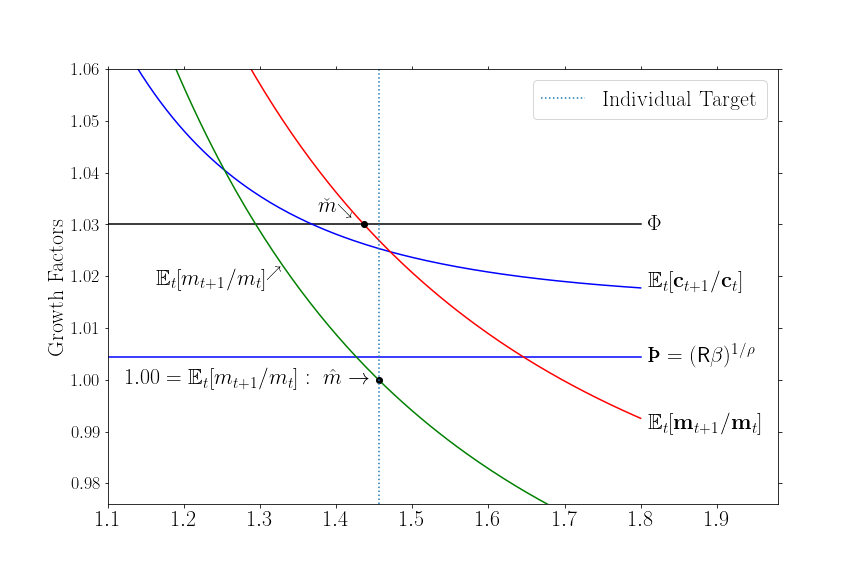
\includegraphics[width=8in]{\FigDir/cNrmTargetFig.png}}
\caption{`Stable' $\mNrm$ Values and Expected Growth Rates}
\label{fig:cNrmTargetFig}
\end{figure}
}{
\begin{figure}[tbp]
\centerline{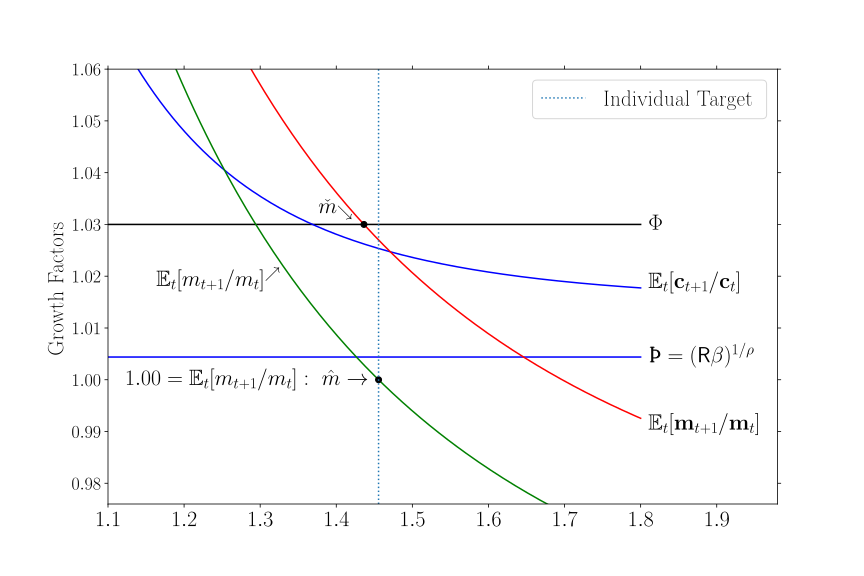
\includegraphics[width=6in]{\FigDir/cNrmTargetFig}}
\caption{`Stable' (Target; Balanced Growth) $\mNrm$ Values}
\label{fig:cNrmTargetFig}
\end{figure}
}


\hypertarget{LimitsAsmtToInfty}{}
\subsection{Limits as \texorpdfstring{$\mNrm$}{m} Approaches Infinity}\label{subsec:LimitsAsmtToInfty}

Define
\begin{align*}
  \ushort{\cFunc}(\mNrm)  & = \MPCmin \mNrm
\end{align*}
which is the solution to an infinite-horizon problem with no noncapital income ($\TranShkAll_{t+n} = 0~\forall~n\geq1$); clearly $\ushort{\cFunc}(\mNrm) < \usual{\cFunc}(\mNrm)$, since allowing the possibility of future noncapital income cannot reduce current consumption.  Our imposition of the {\RIC} guarantees that $\MPCmin > 0$, so this solution satisfies our definition of nondegeneracy, and because this solution is always available it defines a lower bound on both the consumption and value functions.%\footnote{We will assume the \RIC~holds here and subsequently so that $\MPCmin > 0$; the situation is a bit more complex when the \RIC~does not hold.  In that case the bound on consumption is given by the spending that would be undertaken by a consumer who faced binding liquidity constraints.}

Assuming the {\FHWC}~holds, the infinite horizon perfect foresight solution~\eqref{eq:cFuncPFUnc} constitutes an upper bound on consumption in the presence of uncertainty, since the introduction of uncertainty strictly decreases the level of consumption at any $\mNrm$ (\cite{ckConcavity}).  Thus,
\begin{equation} \label{eq:lowerltupper}
  \begin{split}
    \ushort{\cFunc}(\mNrm) < & \usual{\cFunc}(\mNrm)  < \bar{\cFunc}(\mNrm)  \\
    1 < & \usual{\cFunc}(\mNrm)/\ushort{\cFunc}(\mNrm)  < \bar{\cFunc}(\mNrm)/\ushort{\cFunc}(\mNrm).
  \end{split}
\end{equation}
But
\begin{align*}%  \label{eq:limitlowerupper}
  \lim_{m \uparrow \infty} \bar{\cFunc}(\mNrm)/\ushort{\cFunc}(\mNrm)
  & = \lim_{m \uparrow \infty} (\mNrm -1+ \hNrm)/\mNrm  \\
  & = 1,
\end{align*}
so as $\mNrm \uparrow \infty, \usual{\cFunc}(\mNrm)/\ushort{\cFunc}(\mNrm) \rightarrow 1$, and the continuous differentiability and strict concavity of $\usual{\cFunc}(\mNrm)$ therefore implies
\begin{equation*} % \label{eq:limxtoinftycp}
  \lim_{m \uparrow \infty} \usual{\cFunc}^{\prime}(\mNrm) =
  \ushort{\cFunc}^{\prime}(\mNrm) = \bar{\cFunc}^{\prime}(\mNrm) = \MPCmin
\end{equation*}
because any other fixed limit would eventually lead to a level of consumption either exceeding $\bar{\cFunc}(\mNrm)$ or lower than $\ushort{\cFunc}(\mNrm)$.  Figure~\ref{fig:mpclimits} illustrates these limits by plotting the numerical solution.  

\renewcommand{\figFile}{mpclimits}
\hypertarget{\figFile}{}
\hypertarget{MPCLimits}{}
\begin{figure}
\centerline{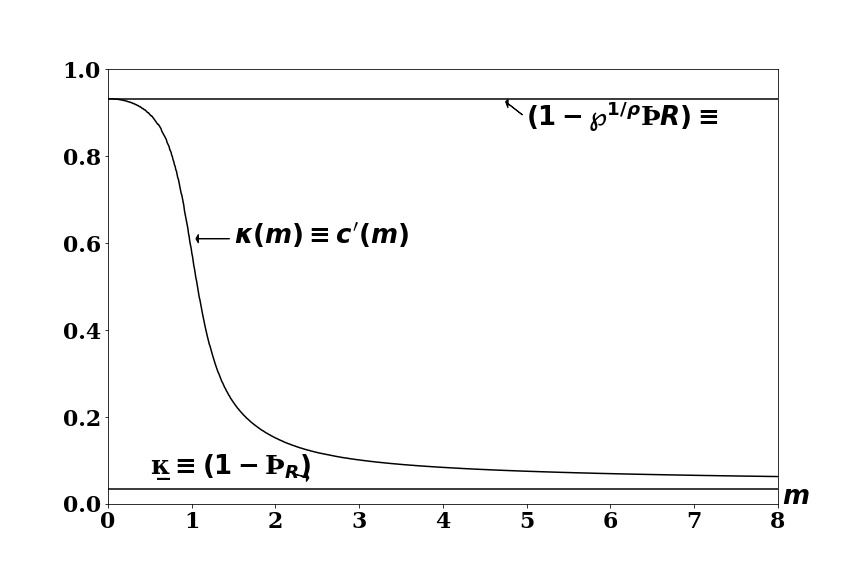
\includegraphics[width=6in]{\FigDir/MPCLimits}}
\caption{Limiting MPC's}
\label{fig:mpclimits}
\end{figure}


\renewcommand{\figFile}{cFuncBounds}
\hypertarget{\figFile}{}
\hypertarget{cFuncBounds}{}
\begin{figure}
\centering
\subfigure[\large Bounds]{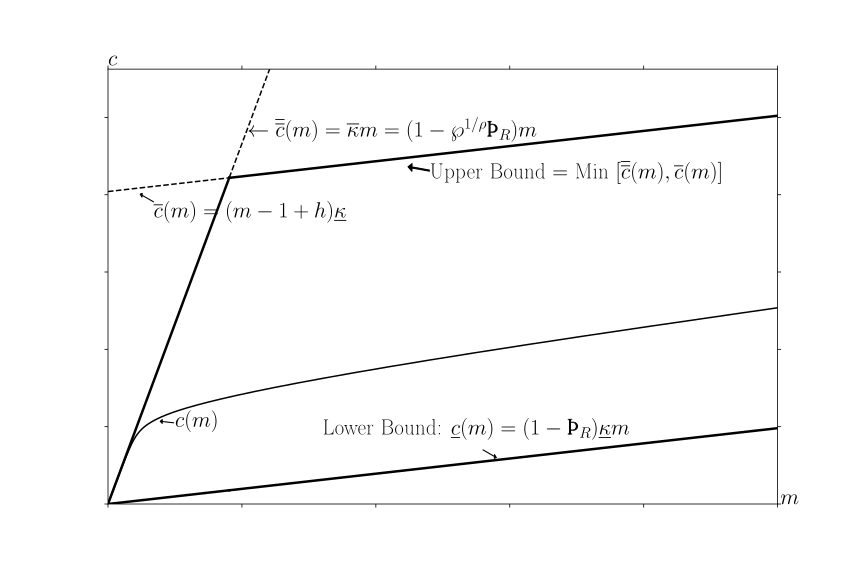
\includegraphics[width=6in]{\FigDir/cFuncBounds}}
\subfigure[\large Target $\mRat$]{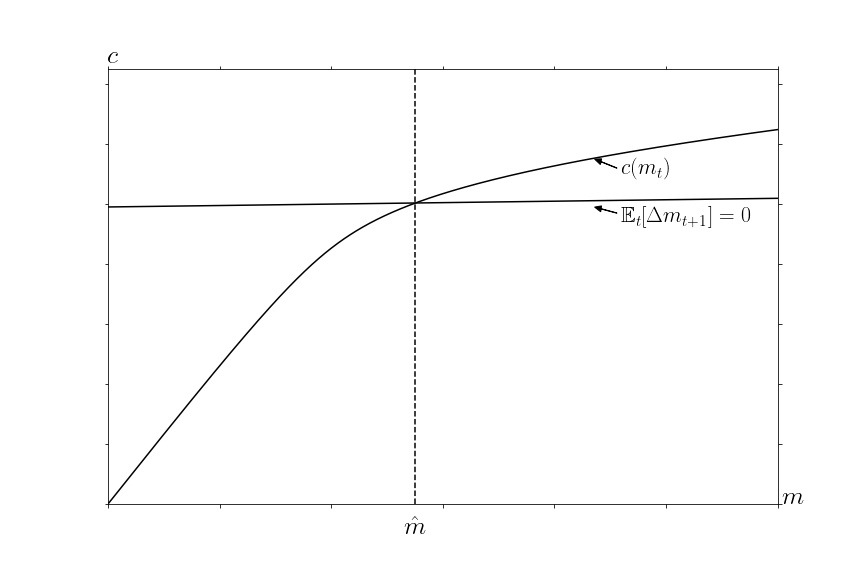
\includegraphics[width=6in]{\FigDir/cRatTargetFig}}
\caption{The Consumption Function}
\label{fig:cFuncBounds}
\end{figure}


Next we establish the limit of the expected consumption growth factor as $\mNrm_{t} \uparrow \infty$:
\begin{align*}
  \lim_{\mNrm_{t} \uparrow \infty} \Ex_{t}[
  \cLvl_{t+1}/\cLvl_{t}]  & = \lim_{\mNrm_{t} \uparrow \infty} \Ex_{t}[
                            {\PermGroFac}_{t+1} {\cNrm}_{t+1}/c_{t}].
\end{align*}

But
\begin{align*}
  \Ex_{t}[{\PermGroFac}_{t+1} {\ushort{\cNrm}}_{t+1}/\bar{\cNrm}_{t}] \leq \Ex_{t}[{\PermGroFac}_{t+1} {\cNrm}_{t+1}/\cNrm_{t}] \leq \Ex_{t}[{\PermGroFac}_{t+1} {\bar{\cNrm}}_{t+1}/\ushort{\cNrm}_{t}]
\end{align*}
and
\begin{equation*}  \label{eq:xttoinfty}
  \lim_{\mNrm_t \uparrow \infty} \PermGroFac_{t+1}\ushort{\cFunc}(\mNrm_{t+1})/\bar{\cFunc}(\mNrm_t) =
  \lim_{\mNrm_{t} \uparrow \infty} \PermGroFac_{t+1}\bar{\cFunc}(\mNrm_{t+1})/\ushort{\cFunc}(\mNrm_t) =
  \lim_{\mNrm_{t} \uparrow \infty}\PermGroFac_{t+1} \mNrm_{t+1}/\mNrm_t,
\end{equation*}
while (for convenience defining $\aFunc(\mNrm_{t})=\mNrm_{t}-\usual{\cFunc}(\mNrm_{t})$), \hypertarget{xtp1toinfty}{}
\begin{align}  \label{eq:xtp1toinfty}
  \lim_{\mNrm_{t} \uparrow \infty} \PermGroFac_{t+1} \mNrm_{t+1}/\mNrm_t  & = \lim_{\mNrm_{t} \uparrow \infty}
                                                                            \left(\frac{\Rfree \aFunc(\mNrm_t)+{\PermGroFac}_{t+1}\TranShkAll_{t+1}}{\mNrm_t}\right)
  \\  & = {(\Rfree \DiscFac)}^{1/\CRRA} = \APFac \notag
\end{align}
because $\lim_{\mNrm_{t}\uparrow \infty} \aFunc^{\prime}(\mNrm)=\RPFac$\footnote{$\displaystyle \lim_{\mNrm_{t}\uparrow \infty} \aFunc(\mNrm_{t})/\mNrm_{t}=1-\lim_{\mNrm_{t}\uparrow \infty} \usual{\cFunc}(\mNrm_{t})/\mNrm_{t}=1-\lim_{\mNrm_{t}\uparrow \infty}\usual{\cFunc}^{\prime}(\mNrm_{t})=\RPFac$.} and $\PermGroFac_{t+1}\TranShkAll_{t+1}/\mNrm_{t} \leq (\PermGroFac \bar{\PermShk} \bar{\TranShkEmp}/\pNotZero )/\mNrm_{t}$ which goes to zero as $\mNrm_{t}$ goes to infinity.

Hence we have
\begin{equation*}
  {\APFac}  \leq \lim_{\mNrm_{t} \uparrow \infty} \Ex_{t}[\cLvl_{t+1}/\cLvl_{t}] \leq {\APFac}
\end{equation*}
so as cash goes to infinity, consumption growth approaches its value $\APFac$ in the perfect foresight model.

\begin{comment}
  Of course, the constraint never becomes irrelevant if human wealth is
  infinite.  We ruled out infinite human wealth at the beginning of this
  section by assuming $\Rfree> \PermGroFac$.  If this finite human wealth
  condition does not hold, it is possible to show that for any finite
  horizon consumer the marginal propensity to consume approaches the
  finite-horizon perfect foresight MPC as wealth approaches infinity.
  However, as the horizon gets longer, the perfect foresight MPC
  approaches zero.  It can be shown therefore that the limiting MPC for
  the converged consumption function approaches (but never reaches)
  zero.  (This is why we chose $\MPCminmin=0$ if the \FHWC~fails
  in the proofs above.)
\end{comment}

\hypertarget{LimitsAsmtToZero}{}
\subsection{Limits as \texorpdfstring{$\mNrm$}{m} Approaches Zero}\label{subsec:LimitsAsmtToZero}

Equation~\eqref{eq:MPCmaxInv} shows that the limiting value of
$\MPCmax$ is
\begin{align*}
  \MPCmax  & = 1-{\Rfree}^{-1}{(\pZero  \Rfree\DiscFac)}^{1/\CRRA}.
\end{align*}

Defining $\eFunc(\mNrm)=\cFunc(\mNrm)/\mNrm$ we have
\begin{align*}
  \lim_{m \downarrow 0} \eFunc(\mNrm)  & = (1-\pZero^{1/\CRRA}\RPFac) = \MPCmax .
\end{align*}

Now using the continuous differentiability of the consumption function along with L'H\^opital's rule, we have
\begin{align*}
  \lim_{m \downarrow 0} \usual{\cFunc}^{\prime}(\mNrm)  & = \lim_{m \downarrow 0}
                                                          \eFunc(\mNrm) = \MPCmax.
\end{align*}

Figure~\ref{fig:mpclimits} visually confirms that the numerical solution obtains this limit for the MPC as $\mNrm$ approaches zero.

For consumption growth, as $\mNrm \downarrow 0$ we have
\begin{align*}
  \lim_{\mNrm_{t} \downarrow 0} \Ex_{t}\left[\left(\frac{\cFunc({\mNrm}_{t+1})}{\cFunc(\mNrm_t)}\right){\PermGroFac}_{t+1}\right]
  & > \lim_{\mNrm_{t} \downarrow 0} \Ex_{t}\left[\left(\frac{\ushort{\cFunc}({\mathcal{\mathcal{R}}}_{t+1}\aFunc(\mNrm_{t})+{%
    \TranShkAll}_{t+1})}{\MPCmax \mNrm_{t}}\right){\PermGroFac}_{t+1}\right]  \notag \\
  & = \pZero \lim_{\mNrm_{t} \downarrow 0} \Ex_{t}\left[\left(\frac{\ushort{\cFunc}({\mathcal{\mathcal{R}}}_{t+1}\aFunc(\mNrm_{t}))}{\MPCmax \mNrm_{t}}\right){\PermGroFac}_{t+1}\right] \\
  & ~~~~~~ + \pNotZero \lim_{\mNrm_{t} \downarrow 0}  \Ex_{t}\left[\left(\frac{\ushort{\cFunc}({\mathcal{\mathcal{R}}}_{t+1}\aFunc(\mNrm_{t})+
    \TranShkEmp_{t+1}/\pNotZero)}{\MPCmax \mNrm_{t}}\right){\PermGroFac}_{t+1}\right]  \\\notag
  & > \pNotZero \lim_{\mNrm_{t} \downarrow 0} \Ex_{t}\left[\left(\frac{\ushort{\cFunc}(
    \TranShkEmp_{t+1}/\pNotZero)}{\MPCmax \mNrm_{t}}\right){\PermGroFac}_{t+1}\right] \\
  & = \infty \nonumber
\end{align*}
where the second-to-last line follows because  $\lim_{\mNrm_{t} \downarrow 0} \Ex_{t}\left[\left(\frac{\ushort{\cFunc}({\mathcal{\mathcal{R}}}_{t+1}\aFunc(\mNrm_{t}))}{\MPCmax \mNrm_{t}}\right){\PermGroFac}_{t+1}\right]$ is positive, and the last line follows because the minimum possible realization of $\TranShkEmp_{t+1}$ is $\ushort{\TranShkEmp}>0$ so the minimum possible value of expected next-period consumption is positive.\footnote{None of the arguments in either of the two prior sections depended on the assumption that the consumption functions had converged.  With more cumbersome notation, each derivation could have been replaced by the corresponding finite-horizon versions.  This strongly suggests that it should be possible to extend the circumstances under which the problem can be shown to define a contraction mapping to the union of the parameter values under which \{\RIC,\FHWC\} hold and \{\FVAC,\WRIC\} hold.  That extension is not necessary for our purposes here, so we leave it for future work.}

\hypertarget{onetarget}{}
\hypertarget{Unique-Stable-Points}{}

\subsection{Unique `Stable' Points}\label{subsec:onetarget}\hypertarget{TheoremTarget}{}

Theorems whose substance is described here (and whose details are in an appendix) articulate alternative (but closely related) stability criteria.

\subsubsection{`Individual Target Wealth' \texorpdfstring{$\mTrgNrm$}{m}}\label{subsubsec:mTarget}
One kind of `stable' point is a `target' value $\mTrgNrm$ such that if $\mNrm_{t}=\mTrgNrm$, then $\Ex_{t}[\mNrm_{t+1}]=\mNrm_{t}$.  Existence of such a target turns out to require the {\GICMod} condition.

\begin{verbatimwrite}{\EqDir/TheoremMTargetIsStable}
  \begin{theorem}\iflabelexists{thm:target}{}{\label{thm:target}} % Don't define it if already defined
    For the nondegenerate solution to the problem defined in Section~\ref{subsec:Setup} when {\FVAC}, {\WRIC}, and {\GICMod} all hold, there exists a unique cash-on-hand-to-permanent-income ratio $\mTrgNrm>0$ such that
    \begin{equation}
      \Ex_t [{\mNrm}_{t+1}/\mNrm_t] = 1 \mbox{~if~} \mNrm_t = \mTrgNrm.
      \iflabelexists{eq:mTarget}{}{\label{eq:mTarget}} % Don't define it if already defined
    \end{equation}
    Moreover, $\mTrgNrm$ is a point of `stability' in the sense that
    \begin{equation}
      \iflabelexists{eq:stability}{}{\label{eq:stability}} % Don't define it if already defined
      \begin{split}
        \forall {\mNrm}_t\in(0,\mTrgNrm),      \,\,& \Ex_t [{\mNrm}_{t+1}] > {\mNrm}_t  \\
        \forall {\mNrm}_t\in(\mTrgNrm,\infty), \,\,& \Ex_t [{\mNrm}_{t+1}] < {\mNrm}_t.
      \end{split}
    \end{equation}
  \end{theorem}
\end{verbatimwrite}
  \begin{theorem}\label{thm:target}
    For the nondegenerate solution to the problem defined in Section~\ref{subsec:Setup} when {\FVAC}, {\WRIC}, and {\GICNrm} all hold, there exists a unique cash-on-hand-to-permanent-income ratio $\mTrg>0$ such that
    \begin{equation}
      \Ex_t [{\mRat}_{t+1}/\mRat_t] = 1 \mbox{~if~} \mRat_t = \mTrg.
      \label{eq:mTarget}
    \end{equation}
    Moreover, $\mTrg$ is a point of `wealth stability' in the sense that
    \begin{equation} \label{eq:stability}
      \begin{split}
        \forall {\mRat}_t\in(0,\mTrg),      \,\,& \Ex_t [{\mRat}_{t+1}] > {\mRat}_t  \\
        \forall {\mRat}_t\in(\mTrg,\infty), \,\,& \Ex_t [{\mRat}_{t+1}] < {\mRat}_t.
      \end{split}
    \end{equation}
  \end{theorem}


\hypertarget{mTargImplicit}{}

Since $\mNrm_{t+1}=(\mNrm_{t}-\cFunc(\mNrm_{t}))\RNrm_{t+1}+\TranShk_{t+1}$, the implicit equation for $\mTrgNrm$ is
\begin{equation} \label{eq:mTargImplicit}
  \begin{split}
    \Ex_{t}[(\mTrgNrm-\cFunc(\mTrgNrm))\RNrm_{t+1}+\TranShk_{t+1}] & = \mTrgNrm
    \\   (\mTrgNrm-\cFunc(\mTrgNrm))\underbrace{\RNrm\Ex_{t}[\PermShk^{-1}]}_{\equiv \bar{\RNrm}}+1 & = \mTrgNrm .
  \end{split}
\end{equation}

This is the most restictive among several competing definitions of stability.  %Parameterizations that satisfy the {\GICMod} are well-behaved for almost any quantitative purpose.

\hypertarget{Collective-Stability}{}
\hypertarget{pseudo-steady-state}{}
\subsubsection{Individual Balanced-Growth `pseudo steady state' \texorpdfstring{$\mBalLvl$}{m}}\label{subsubsec:mSteadyState}
Our least restrictive definition of `stability' derives from a traditional question in macro models: whether there is a `balanced growth' equilibrium in which aggregate variables (income, consumption, market resources) all grow forever by the same factor $\PermGroFac$.  For our model, Figure~\ref{fig:cNrmTargetFig} showed that there is no single $\mNrm$ for which $\Ex_{t}[\mLvl_{t+1}]/\mLvl_{t} = \Ex_{t}[\cLvl_{t+1}]/\cLvl_{t} = \PermGroFac$~for an individual consumer.  Nevertheless, the next section will show that economies populated by heterogeneous collections of such consumers can exhibit balanced growth in the aggregate, and in the cross-section of households.

As an input to that analysis, we show here that if the {\GICRaw} holds, the problem will exhibit a balanced-growth `pseudo-steady-state' point, by which we mean that there is some ${\mBalLvl}$ such that, for all $\mNrm_{t}>{\mBalLvl}$, $\Ex_{t}[\mLvl_{t+1}/\mLvl_{t}] < \PermGroFac$, and conversely if $\mNrm_{t}<{\mBalLvl}$ then $\Ex_{t}[\mLvl_{t+1}/\mLvl_{t}] > \PermGroFac$.

\hypertarget{balgrostable}{}
\hypertarget{balgrostableSolve}{}

The critical $\mNrm$ will be the $\mBalLvl$ at which $\mLvl$ growth matches $\PermGroFac$:
\begin{equation}\label{eq:balgrostable}
  \begin{split}
    \Ex_{t}[\mLvl_{t+1}]/\mLvl_{t} & =\Ex_{t}[\PermLvl_{t+1}]/\PermLvl_{t}
    \\  \Ex_{t}[\mNrm_{t+1}\PermGroFac\PermShk_{t+1}\PermLvl_{t}]/(\mNrm_{t}\PermLvl_{t}) & =\Ex_{t}[\PermLvl_{t}\PermGroFac\PermShk_{t+1}]/\PermLvl_{t}
    \\ \Ex_{t}\left[\PermShk_{t+1}\underbrace{\left((\mNrm_{t}-\usual{\cFunc}(\mNrm_{t})\Rfree/(\PermGroFac\PermShk_{t+1}))+\TranShk_{t+1}\right)}_{\mNrm_{t+1}}\right]/\mNrm_{t} & = 1
    \\ 
    \Ex_{t}\left[(\mBalLvl-\usual{\cFunc}(\mBalLvl))\overbrace{\Rfree/\PermGroFac}^{\RNrm}+\PermShk_{t+1}\TranShk_{t+1}\right] & = \mBalLvl
    \\  (\mBalLvl-\usual{\cFunc}(\mBalLvl))\RNrm+ 1 & = \mBalLvl .
  \end{split}
\end{equation}

The only difference between~\eqref{eq:balgrostable} and~\eqref{eq:mTargImplicit} is the substitution of $\RNrm$ for $\bar{\RNrm}$.\footnote{A third `stable point' is the $\mBalLog$ where $\Ex_{t}[\log \mLvl_{t+1}] = \log \PermGroFac \mLvl_{t}$; this can be conveniently rewritten as $\Ex_{t}\left[\log\left((\mBalLog-\usual{\cFunc}(\mBalLog))\RNrm+\PermShk_{t+1}\TranShk_{t+1}\right)\right]  = \log \mBalLog_{t}$.  Because the expectation of the log of a stochastic variable is less than the log of the expectation, if a solution for $\mBalLog$ exists it will satisfy $\mBalLog > \mBalLvl$; in turn, if $\mTrgNrm$ exists, $\mTrgNrm>\mBalLog$.  $\mBalLog$ is guaranteed to exist when the~{\GICSdl}~condition is satisfied (see below).  For our purposes, little would be gained by an analysis of this point parallel to those of the other points of stability; but to accommodate potential practical uses,  the {\ARKurl} toolkit computes the value of this point (when it exists) as \texttt{mBalLog}.}$^{,}$\footnote{Our choice to call to this the individual problem's `individual balanced-growth pseudo-steady-state' $\mBalLvl$ is motivated by what happens in the case where all draws of all future shocks just happen to take on their expected value of 1.0.  (They unexpectedly always take on their expected values).  In that infinitely improbable case, the economy \textit{would} exhibit balanced growth:
  \begin{align*}
    \Ex_{t}[\mNrm_{t+1}/\mNrm_{t}|\PermShk_{t+1}=\TranShk_{t+1}=1] = \PermGroFac \left(\mBalLvl-\cFunc(\mBalLvl)\RNrm + 1 \right)/\mNrm = \PermGroFac.
  \end{align*}}

%Theorem~\ref{thm:MSSBalExists}~formally states the relevant proposition.
\begin{verbatimwrite}{\EqDir/TheoremMSSBalExists}
  \begin{theorem}
    \iflabelexists{thm:MSSBalExists}{}{\label{thm:MSSBalExists}} % Don't define it if already defined
    For the nondegenerate solution to the problem defined in Section~\ref{subsec:Setup} when {\FVAC}, {\WRIC}, and {\GICRaw} all hold, there exists a unique pseudo-steady-state cash-on-hand-to-income ratio $\mBalLvl>0$ such that
    \begin{equation}
      \Ex_t [\PermShk_{t+1}{\mNrm}_{t+1}/\mNrm_t] = 1 \mbox{~if~} \mNrm_t = \mBalLvl.
      \iflabelexists{eq:mBalLvl}{}{\label{eq:mBalLvl}} % Don't define it if already defined
    \end{equation}
    Moreover, $\mBalLvl$ is a point of stability in the sense that
    \begin{equation}
      \iflabelexists{eq:stabilityStE}{}{\label{eq:stabilityStE}} % Don't define it if already defined
      \begin{split}
        \forall {\mNrm}_t\in(0,\mBalLvl),      \,\,& \Ex_{t}[\mLvl_{t+1}]/\mLvl_{t} > \PermGroFac \\
        \forall {\mNrm}_t\in(\mBalLvl,\infty), \,\,& \Ex_{t}[\mLvl_{t+1}]/\mLvl_{t} < \PermGroFac.
      \end{split}
    \end{equation}
  \end{theorem}
\end{verbatimwrite}
  \begin{theorem}\label{thm:MSSBalExists}
    For the nondegenerate solution to the problem defined in Section~\ref{subsec:Setup} when {\FVAC}, {\WRIC}, and {\GIC} all hold, there exists a unique pseudo-steady-state cash-on-hand-to-income ratio $\mStE>0$ such that
    \begin{equation}
      \Ex_t [\pShk_{t+1}{\mRat}_{t+1}/\mRat_t] = 1 \mbox{~if~} \mRat_t = \mStE.
      \label{eq:mStE}
    \end{equation}
    Moreover, $\mStE$ is a point of stability in the sense that
    \begin{equation}\label{eq:stabilityStE}
      \begin{split}
        \forall {\mRat}_t\in(0,\mStE),      \,\,& \Ex_{t}[\mLevBF_{t+1}]/\mLevBF_{t} > \PGro \\
        \forall {\mRat}_t\in(\mStE,\infty), \,\,& \Ex_{t}[\mLevBF_{t+1}]/\mLevBF_{t} < \PGro.
      \end{split}
    \end{equation}
  \end{theorem}



\begin{comment}
  \hypertarget{log-pseudo-steady-state}{}
  \subsubsection{The  expected `log-pseudo steady state'}\label{subsubsec:logpseudosteadystate}

  A final point of stability will be indicated by a $\sim$ accent; this is the $\mNrm$ at which the expectation of $\log \mLvl$ is unchanging.

  \begin{verbatimwrite}{\EqDir/TheoremGroIsStable}
    \begin{theorem}\iflabelexists{thm:TheoremGroIsStable}{}{\label{thm:TheoremGroIsStable}}
      For the nondegenerate solution to Section~\ref{subsec:Setup}'s problem when {\FVAC}, {\WRIC}, and {\GICRaw} all hold, there exists a unique cash-on-hand-to-permanent-income ratio $\mBalLvl>0$ such that
      \begin{equation}
        \Ex_t [\log {\mLvl}_{t+1} ] = \log \mLvl_t \mbox{~if~} \mLvl_t = \mBalLvl.
        \iflabelexists{eq:mTarget}{}{\label{eq:mTarget}}
      \end{equation}
      Moreover, $\mBalLvl$ is a point of stability in the sense that
      \begin{equation} \label{eq:stabilityLog}
        \begin{split}
          \forall {\mNrm}_t\in(0,\mBalLvl),      \,\,& \Ex_t [\log {\mLvl}_{t+1}] > \log {\mLvl}_t  \\
          \forall {\mNrm}_t\in(\mBalLvl,\infty), \,\,& \Ex_t [\log {\mLvl}_{t+1}] < \log {\mLvl}_t.
        \end{split}
      \end{equation}
    \end{theorem}
  \end{verbatimwrite}
    \begin{theorem}\label{thm:TheoremGroIsStable}
    For the nondegenerate solution to the problem defined in Section~\ref{subsec:Setup} when {\FVAC}, {\WRIC}, and {\GICLog} all hold, there exists a unique cash-on-hand-to-permanent-income ratio $\mGro>0$ such that
    \begin{equation}
      \Ex_t [\log {\mLvl}_{t+1} ] = \log \mLvl_t \mbox{~if~} \mLvl_t = \mGro.
      \label{eq:mTarget}
    \end{equation}
    Moreover, $\mGro$ is a point of stability in the sense that
    \begin{equation} \label{eq:stability}
      \begin{split}
        \forall {\mNrm}_t\in(0,\mGro),      \,\,& \Ex_t [\log {\mLvl}_{t+1}] > \log {\mLvl}_t  \\
        \forall {\mNrm}_t\in(\mGro,\infty), \,\,& \Ex_t [\log {\mLvl}_{t+1}] < \log {\mLvl}_t.
      \end{split}
    \end{equation}
  \end{theorem}


  with two associated Lemmas demonstrating that $\mBalLvl < \mBalLog$ and $\mBalLvl < \$\mTrgNrm$.
\end{comment}

The proofs of these theorems are intuitive, and almost completely parallel; to save space, they are relegated to Appendix~\ref{sec:ApndxMTargetIsStable}.  They involve three steps:
\begin{enumerate}
\item Existence and continuity of $\Ex_{t}[\mNrm_{t+1}/\mNrm_{t}]$ or $\Ex_{t}[\mNrm_{t+1}\PermShk_{t+1}/\mNrm_{t}]$
  \begin{itemize}
  \item This follows from existence and continuity of the constituents
  \end{itemize}
\item Existence of the equilibrium point
  \begin{itemize}
  \item This follows from existence of upper and lower bound limiting MPCs, existence and continuity of the decision rule, and the Intermediate Value Theorem
  \end{itemize}
\item Monotonicity of $\Ex_{t}[{\mNrm}_{t+1}-\mNrm_{t}]$ or $\Ex_{t}[{\mNrm}_{t+1}\PermShk_{t+1}-\mNrm_{t}]$
  \begin{itemize}
  \item This follows from concavity of the consumption function
  \end{itemize}
\end{enumerate}

\subsection{Example With Balanced-Growth \texorpdfstring{$\mBalLvl$}{m} But No Target~\texorpdfstring{$\mTrgNrm$}{m}}

Because the equations defining target and pseudo-steady-state $\mNrm$,~\eqref{eq:mTargImplicit} and~\eqref{eq:balgrostable}, differ only by substitution of $\RNrm$ for $\bar{\RNrm}=\RNrm \Ex[\PermShk^{-1}]$, if there are no permanent shocks ($\PermShk \equiv 1$), the conditions are identical.  For many parameterizations (e.g., under the baseline parameter values used for constructing figure~\ref{fig:cNrmTargetFig}), $\mTrgNrm$ and $\mBalLvl$ will not differ much.

\renewcommand{\figFile}{GICModFailsButGICRawHolds}
\hypertarget{\figFile}{}
 % Store the tex for standalone compilation
\begin{figure}[tbp]
\centerline{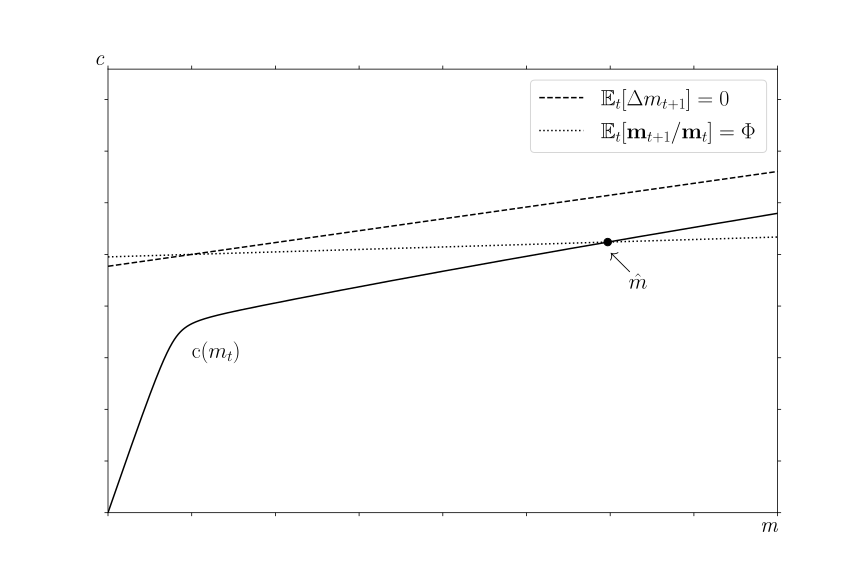
\includegraphics[width=6in]{\FigDir/GICModFailsButGICRawHolds}}
%\caption{\{{FVAC},{GIC},\cncl{GIC-Mod}\}: No $\TargetNrm{\mNrm}$ Exists But $\BalGroFac{\mNrm}$ Does}
\caption{\{{FVAC},{GIC},\cncl{GIC-Mod}\}: No Target Exists But SS Does}
\label{fig:GICModFailsButGICRawHolds}
\end{figure}


An illuminating exception is exhibited in Figure~\ref{fig:GICModFailsButGICRawHolds}, which modifies the baseline parameter values by quadrupling the variance of the permanent shocks, enough to cause failure of the \GICMod; now there is no target wealth level $\mTrgNrm$.  But the pseudo-steady-state still exists because it turns off realizations of the permanent shock.  It is tempting to conclude that the reason target $\mTrgNrm$ does not exist is that the increase in the size of the shocks induces a precautionary motive that increases the consumer's effective patience.  But that interpretation is not correct when the {\FHWC} holds, because as market resources approach infinity, precautionary saving against noncapital income risk becomes negligible (as the proportion of consumption financed out of such income approaches zero).  The correct explanation is more prosaic: The increase in uncertainty boosts the expected uncertainty-modified rate of return factor from $\RNrm$ to $\bar{\RNrm}>\RNrm$ which reflects the fact that in the presence of uncertainty the expectation of the inverse of the growth factor increases: $\PermGroFacAdj > \PermGroFac$.  That is, in the limit as $\mNrm \uparrow \infty$ the increase in effective impatience reflected in $\GPFacNrm < \GPFacRaw$ is entirely due to the certainty-equivalence growth adjustment, not to a (limiting) change in precaution.  In fact, the next section will show that an aggregate balanced growth equilibrium will exist even when realizations of the permanent shock are not turned off: The required condition for aggregate balanced growth is the regular {\GICRaw}, which ignores the magnitude of permanent shocks, not the {\GICMod}.\footnote{\cite{szeidlInvariant}'s impatience condition, discussed below, also tightens as uncertainty increases, but this is also not a consequence of a precaution-induced increase in patience -- it represents an increase in the tightness of the requirements of the `mixing condition' used in his proof.}

Before we get to the formal arguments, the key insight can be understood by considering an economy that starts, at date $t$, with the entire population at $\mNrm_{t}=\mBalLvl$, but then evolves according to the model's assumed dynamics between $t$ and $t+1$.  Equation~\eqref{eq:balgrostable} will still hold, so for this first period, at least, the economy will exhibit balanced growth: the growth factor for aggregate $\mLvl$ will match the growth factor for permanent income $\PermGroFac$.  It is true that there will be people for whom $\bNrm_{t+1}=\aNrm_{t}\Rfree/(\PermGroFac\PermShk_{t+1})$ is boosted by a small draw of $\PermShk_{t+1}$.  But their contribution to the \textit{level} of the aggregate variable is given by $\bLvl_{t+1}=\bNrm_{t+1}\PermShk_{t+1}$, so their $\bNrm_{t+1}$ is reweighted by an amount that exactly unwinds that divisor-boosting.  This means that it is possible for the consumption-to-permanent-income ratio for every consumer to be small enough that their market resources ratio is expected to rise, and yet for the economy as a whole to exhibit a balanced growth equilibrium with a finite aggregate balanced growth steady state $\BalGroFac{\MNrm}$ (this is not numerically the same as the individual \hyperlink{pseudo-steady-state}{pseudo-steady-state} ratio $\mBalLvl$ because the problem's nonlinearities have consequences when aggregated).\footnote{Still, the pseudo-steady-state can be calculated from the policy function without any simulation, and therefore serves as a low-cost starting point for the numerical simulation process; see \href{https://econ-ark.org/materials/harmenberg-aggregation?launch}{Harmenberg-Aggregation} for an example.}



\hypertarget{The-Aggregate-and-Idiosyncratic-Relationship-Between-Consumption-Growth-and-Income-Growth}{}
\section{Invariant Relationships}

% A large (infinite) collection of small (infinitesimal) buffer-stock consumers with identical parameter values can be thought of as a subset of the population within a single country (say, members of a given education or occupation group), or as the whole population in a small open economy with an exogenous (constant) interest rate.\footnote{It is also possible, and only slightly more difficult, to solve for the steady-state of a closed-economy version of the model where the interest rate is endogenous.}

% Until now for convenience we have assumed infinite horizons, with the implicit understanding that white noise mortality could be handled by adjusting the effective discount factor.  On that basis, Section~\ref{subsec:cGroEqPermGroFacIndQ} continues to omit mortality.  But a reason mortality may be useful will appear at the end of Section~\ref{subsec:cGroEqPermGroFacQ}, so alternative mortality treatments are briefly examined in section~\ref{sec:Mortality-And-Redistribution}.

% Attanasio and Weber~\citeyearpar{aw95} point out that concavity of the consumption function can imply that it is quantitatively important to distinguish between the growth rate of average consumption and the average growth rate of  consumption.\footnote{Since we assume number of the households are   normalized to 1, aggregate and average variables are identical.}  We have just examined the average growth rate; we now examine the growth rate of the average.

% Microeconomic distributional relationships are increasingly central to macroeconomic research (see, e.g., \cite{violante_marginal_2021}'s recent Laffont lectures on relationship between the marginal propensity to consume and the distribution of assets).  But mapping from micro data to macro models can be subtle.  Hence this final section's aim of carefully describing those relationships in the paper's simple model.

Assume a continuum of \textit{ex ante} identical buffer-stock households on the unit interval, with constant total mass normalized to one and indexed by $i \in [0,1]$.% (all behaving according to the model specified above).

Szeidl~\citeyearpar{szeidlInvariant} proved that such a population will be characterized by invariant distributions of $\mNrm$, $\cNrm$, and $\aNrm$ under the condition\footnote{\cite{szeidlInvariant}'s equation (9), in our notation, is:
  \begin{align*}
    \Ex \log \Rfree (1-\MPC) & < \Ex \log \PermGroFac \PermShk
    \\  \Ex \log \Rfree \RPFac  &  < \Ex \log \PermGroFac \PermShk
    \\ \log \GPFacRaw & < \Ex \log \PermShk
  \end{align*}
  which, exponentiated, yields~\eqref{eq:GICSdl}.}
\hypertarget{GICSdl}{}
\begin{align}
  \text{\GICSdl:~~}  \log~\GPFacRaw & < \Ex [\log \PermShk] \label{eq:GICSdl}
\end{align}
which is stronger than our {\GICRaw} ($\GPFacRaw < 1$), but weaker than our {\GICMod} ($\GPFacNrm < 1$).\footnote{Under our default (though not required) assumption that $\log \PermShk \sim \mathcal{N}(-\sigma^{2}_{\PermShk}/2,\sigma^{2}_{\PermShk})$; the {\GICMod} in this case, is $\GPFacRaw < \exp(-\sigma^{2})$, so if the {\GICMod} holds then Szeidl's condition will hold.}  %Below we designate these the `Szeidl-invariant' distributions $\Nvrnt({\mNrm})$, $\Nvrnt({\aNrm})$, and $\Nvrnt({\cNrm})$.%\footnote{Szeidl's proof supplants simulation evidence of ergodicity that appeared in an earlier version of this paper.}

\hypertarget{Growth-Rates-of-Aggregate-Income-and-Consumption}{}

\cite{harmenbergInvariant} substitutes a clever change of probability-measure into Szeidl's proof, with the implication that if the {\GICRaw} holds, invariant \emph{permanent-income-weighted} distributions exist.  %In a nutshell:\footnote{See \ref{sec:ApndxHarKmenberg} for a less abbreviated treatment in this paper's notation.} If $\PermShk$ is described by density function $f_\PermShk(\PermShk)$, Harmenberg defines the \emph{permanent-income-neutral measure} by $\Harm{f}_\PermShk(\PermShk) \equiv \PermShk f_\PermShk(\PermShk)$.  Following derivations parallel to those in the previous footnote, the condition for the existence of invariant permanent-income-weighted distributions is\hypertarget{GICHarm}{}
% \begin{align} 
%    \text{\GICHarm:~~} \log \GPFacRaw  & < \Harm{\Ex}[ \log \PermShk] \label{eq:GICHarm}
% \end{align}
% where the {$\sim$} over the expectations operator indicates that the expectation is being taken with respect to $\Harm{f}_{\PermShk}(\PermShk)$.  Under our baseline assumption that the permanent shocks are lognormally distributed, it is possible to show that $\Harm{\Ex} [\log \PermShk] = \PermShkStd^{2}/2,$ so exponentiating both sides of this equation turns it into $\GPFacRaw < e^{\PermShkVar/2}$ which is \textit{weaker} than the {\GICRaw} because $1 < e^{\PermShkVar/2}$.\footnote{{\GICHarm} is always weaker than the {\GICRaw} because $x \log x$ is a convex function, so the expectation of the permanent-income-weighted distribution is always greater when there is risk than in the absence of risk (thanks again to the invaluable Mr Jensen).}$^{,}$\footnote{The fact that }
This allows him to prove a conjecture from an earlier draft of this paper (\cite{BufferStockTheoryQESubmit}) that under the {\GICRaw}, aggregate consumption grows at the same rate $\PermGroFac$ as aggregate noncapital income in the long run (with the corollary that aggregate assets and market resources grow at that same rate). \hypertarget{test-Harmenbergs-method}{}
% Given the terminology developed earlier, the natural designation for the stable ratio of aggregate market resources to noncapital income is the `aggregate steady state' ratio, $\BalGroFac{M}$.  This is not numerically the same as the individual \hyperlink{pseudo-steady-state}{pseudo-steady-state} ratio $\mBalLvl$ because the nonlinearities involved in simulation and aggregation will have consequences.\footnote{Still, the pseudo-steady-state can be calculated immediately from the policy function without any simulation, and therefore would likely serve as an excellent and low-cost starting point for the numerical simulation process.}
\cite{harmenbergInvariant} shows that his reformulation of the problem can reduce costs of calculation enormously.\footnote{The Harmenberg method is implemented in the {\ARKurl}; see the last part of \href{https://github.com/econ-ark/BufferStockTheory/blob/master/Code/Python/test_Harmenbergs_method.sh}{\texttt{test\_Harmenbergs\_method.sh}}.}  \href{https://econ-ark.org/materials/harmenberg-aggregation}{In confirmation, this notebook} finds that the Harmenberg method reduces the simulation size required for a given degree of accuracy by roughly a factor of 100 (!) under the baseline parameter values defined above.% The idea also appears to be promisingly generalizable: For any statistic $\mathcal{S}$ that is the key focus of an analysis, it should be possible to improve the efficiency of simulations aimed at calculating that statistic by constructing an $\mathcal{S}$-weighted distribution rather than a neutral distribution.

%Such an economy will exhibit an \textit{aggregate} `steady-state' ratio of market resources to income $\MBalLvl$ (different from the individual `pseudo-steady-state' $\mBalLvl$).  Corresponding ratios for $\CLvl$ and other also exist even if the {\GICRaw} fails (so that the idiosyncratic pseudo-steady-state does not exist).

The remainder of this section briefly draws out some implications of these points.

\hypertarget{Growth-Rates-of-Individual-Income-and-Consumption}{}
\subsection{Individual Balanced Growth of  Income, Consumption, and Wealth}\label{subsec:cGroEqPermGroFacQ}

Define $\Mean\left[\bullet\right]$ to yield the mean of its argument in the population (as distinct from the expectations operator $\Ex\left[\bullet\right]$ which represents beliefs about the future).  Using boldface capitals for aggregates, the growth factor for aggregate noncapital income is:
\begin{align*}
  \YLvl_{t+1}/\YLvl_{t}  & = \Mean\left[\TranShkAll_{t+1}\PermGroFac \PermShk_{t+1}\PermLvl_{t}\right]/\Mean\left[\PermLvl_{t}\TranShkAll_{t}\right]  \\
                         & = \PermGroFac
\end{align*}
because of the independence assumptions we have made about $\TranShkAll$ and $\PermShk$.

Consider an economy that satisfies the Szeidl impatience condition~\eqref{eq:GICSdl} and has existed for long enough by date~$t$ that we can consider it as Szeidl-converged.  In such an economy a microeconomist with a population-representative panel dataset could calculate the growth rate of consumption for each individual household, and take the average:
\begin{equation}\label{eq:MeanDeltaLogC}
  \begin{split}
    \Mean\left[\Delta \log \cLvl_{t+1}\right]  & = \Mean\left[ \log {\cNrm}_{t+1}\PermLvl_{t+1} - \log c_{t}\PermLvl_{t}\right]  \\
        %                            & = \Mean\left[ \log \PermLvl_{t+1}- \log \PermLvl_{t} + \log {\cNrm}_{t+1} - \log c_{t}\right]  \notag \\
    & = \Mean\left[ \log \PermLvl_{t+1}- \log \PermLvl_{t}\right] + \Mean\left[ \log {\cNrm}_{t+1} - \log c_{t}\right].
  \end{split}
\end{equation}

Because this economy is Szeidl-converged, distributions of $\cNrm_{t}$ and $\cNrm_{t+1}$ will be identical, so that the second term in  \eqref{eq:MeanDeltaLogC} disappears; hence, mean cross-sectional growth rates of consumption and permanent income are the same:
\begin{align}
  \Mean\left[\Delta \log \cLvl_{t+1}\right]  & = \Mean\left[ \Delta \log \PermLvl_{t+1}\right] = \log \PermGroFac \label{eq:MeanDeltaLogCeqMeanDeltaLogP}.
\end{align}

In a Harmenberg-invariant economy (and therefore also any Szeidl-invariant economy), a similar proposition holds in the cross-section as a direct implication of the fact that a constant proportion of total permanent income is accounted for by the successive sets of consumers with any particular $\mNrm$.  This fact is one way of interpreting Harmenberg's definition of the density of the permanent-income-invariant distribution of $\mNrm$; call this density~$\pHarm(\mNrm)$.\footnote{In his notation, this is $\tilde{\psi}^{\mNrm}$.}  Call $\cLvl_{t}(\mNrm)$ the total amount of consumption at date $t$ by persons with market resources $\mNrm$, and note that in the invariant economy this is given by the converged consumption function $\cFunc(\mNrm)$ multiplied by the amount of permanent income accruing to such people $\pHarm(\mNrm)\PermLvl_{t}$.  Since $\pHarm(\mNrm)$ is invariant and aggregate permanent income grows according to $\permLvlAgg_{t+1} = \PermGroFac \permLvlAgg_{t}$, for any $\mNrm$:
\begin{equation*}
  \begin{split}
    \log \cLvl_{t+1}(\mNrm) - \log \cLvl_{t}(\mNrm) &  \notag
    = \log \cFunc(\mNrm) \pHarm(\mNrm)\permLvlAgg_{t+1} - \log \cFunc(\mNrm)\pHarm(\mNrm)\permLvlAgg_{t} \\
    & = \log \PermGroFac.
  \end{split}
\end{equation*}



\hypertarget{Balanced-Growth-Of-Covariances}{}
\subsection{Aggregate Balanced Growth and Idiosyncratic Covariances}\label{subsec:Covariances}

Harmenberg shows that the covariance between the individual consumption ratio $\cNrm$ and the idiosyncratic component of permanent income $\PermLvl$ does not shrink to zero; thus, covariances are another potential measurement for construction of microfoundations.  % Here we draw out some of those implications.

Consider a date-$t$ Harmenberg-converged economy, and define the mean value of the consumption ratio as $\cNrmAvg_{t+n} \equiv \Mean[\cNrm_{t+n}]$.  Normalizing period-$t$ aggregate permanent income to $\permLvlAgg_{t}=1$, total consumption at $t+1$ and $t+2$ are
\begin{equation}\label{eq:atp2vsatp1}
  \begin{split}
      %       \CLvl_{t}  % & l= \bar{\tilde{\cNrm}}_{t} = \Mean[\cNrm_{t}\PermLvl_{t}] = \Mean[\cNrm_{t}]\Mean[\PermLvl_{t}] + \cov_{t}(\cNrm_{t}, \PermLvl_{t}) \\
        %                            & = %\bar{\tilde{\cNrm}}_{t} =
                                       %                                        \Mean[\cNrm_{t}\PermLvl_{t}] = \Mean[\cNrm_{t}]\overbrace{\Mean[\PermLvl_{t}]}^{=1} + \cov_{t}(\cNrm_{t}, \PermLvl_{t})  \\
    \CLvl_{t+1} & = \Mean[\cNrm_{t+1}\PermLvl_{t+1}] = \cNrmAvg_{t+1}\PermGroFac^{1} + \cov_{t+1}(\cNrm_{t+1}, \PermLvl_{t+1})
    \\  \CLvl_{t+2} & = \Mean[\cNrm_{t+2}\PermLvl_{t+2}] = \cNrmAvg_{t+2}\PermGroFac^{2} + \cov_{t+2}(\cNrm_{t+2}, \PermLvl_{t+2})
  \end{split}
\end{equation}
and Harmenberg's proof that $\CLvl_{t+2}-\PermGroFac \CLvl_{t+1}=0$ allows us to obtain:
\begin{equation} \label{eq:cNrmvsCov}\begin{split}
                      %                       0 & = \cNrmAvg_{t+2}\PermGroFac^{2} + \cov_{t+2}-\PermGroFac\left(\PermGroFac\cNrmAvg_{t+1} + \cov_{t+1}\right)\\ %
        %         \cNrmAvg_{t+2}\PermGroFac^{2} + \cov_{t+2}   & =\cNrmAvg_{t+1}\PermGroFac^{2} + \PermGroFac \cov_{t+1}\\
    \left(\cNrmAvg_{t+2} - \cNrmAvg_{t+1}\right)\PermGroFac^{2} & = \PermGroFac \cov_{t+1} - \cov_{t+2} .
  \end{split}\end{equation}

In a Szeidl-invariant economy, $\cNrmAvg_{t+2} = \cNrmAvg_{t+1}$, so the economy exhibits balanced growth in the covariance:
\begin{align}
  \cov_{t+2} & = \PermGroFac \cov_{t+1}.
\end{align}

The more interesting case is when the economy is Harmenberg- but not Szeidl-invariant.  In that case, if the $\cov$ and the $\cNrmAvg$ terms have constant growth factors $\GroFac_{\cov}$ and $\GroFac_{\cNrmAvg}$,\footnote{This `if' is a conjecture, not something proven by Harmenberg (or anyone else).  But see appendix~\ref{sec:ApndxBalancedGrowthcNrmAndCov} for an example of a Harmenberg-invariant economy in which simulations suggest this proposition holds.} an equation corresponding to \eqref{eq:cNrmvsCov} will hold in $t+n$:
\begin{equation} \label{eq:aNrmGrovsCovGronm1}
  \begin{split}
    (\overbrace{\GroFac_{\cNrmAvg}^{n}\cNrmAvg_{t}}^{\cNrmAvg_{t+n}}-\GroFac^{n-1}_{\cNrm}\cNrmAvg_{t})\PermGroFac^{n} & = \left(\PermGroFac\GroFac_{\cov}^{n-1} -\GroFac_{\cov}^{n}\right)\cov_{t}
    \\ (\GroFac_{\cNrmAvg}\PermGroFac)^{n-1} (\GroFac_{\cNrmAvg}-1)\cNrmAvg_{t}\PermGroFac & = \GroFac_{\cov}^{n-1}(\PermGroFac - \GroFac_{\cov}) \cov_{t}
  \end{split}
\end{equation}
so for the LHS and RHS to grow at the same rates we need
\begin{align}
  \GroFac_{\cov}  & = \GroFac_{\cNrmAvg}\PermGroFac \label{eq:aNrmGrovscovGro}.
\end{align}
This is intuitive:  In the Szeidl-invariant economy, it just reproduces our result above that the covariance exhibits balanced growth because $\GroFac_{\cNrmAvg}=1$.  The revised result just says that in the Harmenberg case where the mean value $\cNrmAvg$ of the consumption ratio $\cNrm$ can grow, the covariance must rise in proportion to any ongoing expansion of $\cNrmAvg$ (as well as in proportion to the growth in $\PermLvl$).

\begin{comment}
  \begin{align*}
    \overbrace{\GroFac_{\cNrmAvg}^{n} \cNrmAvg_{t}}^{\cNrmAvg_{t+n}}(\GroFac_{\cNrmAvg} - 1)\PermGroFac^{n} & =(\GroFac_{\cov} - \PermGroFac) \overbrace{\cov_{t}\GroFac_{\cov}^{n}}^{\cov_{t+n}}
    \\
    (\GroFac_{\cNrmAvg}\PermGroFac/\GroFac_{\cov})^{n} \cNrmAvg_{t}(\GroFac_{\cNrmAvg} - 1) & =(\GroFac_{\cov} - \PermGroFac) \cov_{t}
  \end{align*}
  and a corresponding equation will hold in $t+1$:
  \begin{align*}
    \\  \overbrace{\GroFac_{\cNrmAvg} \cNrmAvg_{t}}^{\cNrmAvg_{t+1}}(\GroFac_{\cNrmAvg} - 1)\PermGroFac & =(\GroFac_{\cov} - \PermGroFac) \overbrace{\cov_{t}\GroFac_{\cov}}^{\cov_{t+1}}
  \end{align*}
  \begin{align*}
    (\GroFac_{\cNrmAvg} - 1)\cNrmAvg_{t}(\GroFac_{\cNrmAvg} - 1)\PermGroFac & =(\GroFac_{\cov} - \PermGroFac) \cov_{t}(\GroFac_{\cov} - 1)
  \end{align*}

  \begin{align*}
    (\GroFac_{\cNrmAvg} - 1)\cNrmAvg_{t}(\GroFac_{\cNrmAvg} - 1)\PermGroFac & =(\GroFac_{\cov} - \PermGroFac) \cov_{t}(\GroFac_{\cov} - 1)
  \end{align*}
  \begin{align}
                                                                              %                                                                               \GroFac_{\cNrmAvg} - 1 & = \GroFac_{\cov} - \PermGroFac \\
        %         \GroFac_{\cNrmAvg} + \PermGroRte & = \GroFac_{\cov}  \\
    \GroFac_{\cov} & = \GroFac_{\cNrmAvg} + (\PermGroFac - 1) \label{eq:aNrmGroVscov}
  \end{align}
  \begin{align*}
    \CLvl_{t}  % & l= \bar{\tilde{\cNrm}}_{t} = \Harm{\Mean}_{t+1}[\cNrm_{t}\PermLvl_{t}] = \Harm{\Mean}_{t+1}[\cNrm_{t}]\Harm{\Mean}_{t+1}[\PermLvl_{t}] + \cov_{t}(\cNrm_{t}, \PermLvl_{t}) \\
                 & = %\bar{\tilde{\cNrm}}_{t} =
                   \Harm{\Mean}_{t\phantom{+1}}[\cNrm]\phantom{\PermGroFac} = \Mean[\cNrm_{t\phantom{t+1}}]\phantom{\PermGroFac} + \cov_{t}(\cNrm_{t}, \PermLvl_{t})  \\
    \CLvl_{t+1} & = \Harm{\Mean}_{t         +1 }[\cNrm]         \PermGroFac  = \cNrmAvg_{t+1}\PermGroFac  + \cov_{t+1}(\cNrm_{t+1}, \PermLvl_{t+1})
  \end{align*}

  Still, both of these quantitites are in priniciple measurable in microdata.  %Indeed, in principle, the Harmenberg-invariant distribution itself could be measured in such data.

\end{comment}

\begin{comment}
  which is the point where $\HarmWide{\cov}_{t}$ is the covariance calculated according to the Harmenberg measure.

  As Harmenberg points out, a convenient feature of his measure is that $\Harm{\Mean}_{t+n}[\PermLvl_{t+n}]=\PermGroFac^{n}$.  Using this, if by date $t=0$ the economy had achieved a Harmenberg-invariant state then we could define $\cNrmAvg=\Harm{\Mean}_{t}[\cNrm_ {t}]$ and use the fact that thereafter assets grow at the constant rate $\PermGroFac$ to obtain
  \begin{equation}
    \begin{split}\label{eq:covProblem}
      \CLvl_{t+1} & = \PermGroFac \CLvl_{t}\notag \\
      \cNrmAvg\PermGroFac +\HarmWide{\cov}(\cNrm_{t+1},\PermLvl_{t+1})   & = \PermGroFac \left( \cNrmAvg    +  \HarmWide{\cov}(\cNrm_{t},\PermLvl_{t})\right)
      \\  \HarmWide{\cov}(\cNrm_{t+1},\PermLvl_{t+1})   & = \HarmWide{\cov}(\cNrm_{t},\PermLvl_{t})  \notag
    \end{split}
  \end{equation}

  A corresponding argument shows that $\cov(\mNrm,\PermLvl)$ also grows by $\PermGroFac$.
\end{comment}


\hypertarget{microfounding-macro-needs-ergodicity}{}
\subsection{Implications for Microfoundations}\label{subsec:microfoundations}

Thus we have microeconomic propositions, for both growth rates and for covariances of observable variables,\footnote{Parallel results to those for consumption can be obtained for other measures like market assets.} that can be tested in either cross-section or panel microdata to judge (and calibrate) the microfoundations that should hold for any macroeconomic analysis that requires balanced growth for its conclusions.

At first blush, these points are reassuring; one of the most persuasive arguments for the agenda of building microfoundations of macroeconomics is that newly available `big data' allow us to measure cross-sectional covariances with great precision, so that we can use microeconomic natural experiments to disentangle questions that are hopelessly entangled in aggregate time-series data.  Knowing that such covariances ought to be a stable feature of a stably growing economy is therefore encouraging.

But this discussion also highlights an uncomfortable point: In the model as specified, permanent income does not have a limiting distribution; it becomes ever more dispersed as the economy with infinite-horizon consumers continues to exist indefinitely.

A few microeconomic data sources attempt direct measurement of `permanent income'; \cite{cstwMPC}, for example, show that their assumptions about the magnitude of permanent shocks (and mortality; see below) yield a simulated distribution of permanent income that roughly matches answers in the U.S.\ \emph{Survey of Consumer Finances} (`SCF') to a question designed to elicit a direct measure of respondents' permanent income.  They use those results to calibrate a model to match empirical facts about the distribution of permanent income and wealth, showing that the model also does fits empirical facts about the marginal propensity to consume.  The quantitative credibility of the argument depends on the model's match to the distribution of permanent income inequality, which would not be possible in a model without a nondegenerate steady-state distribution of permanent income.

For macroeconomists who want to build microfoundations by comparing the microeconomic implications of their models to micro data (directly -- not in ratios to difficult-to-meaure `permanent income'), it would be something of a challenge to determine how to construct empirical-data-comparable simulated results from a model with no limiting distribution of permanent income.

\begin{comment}
  \hypertarget{Consumption-and-Income-Growth-at-the-Household-Level}{}
  \subsection{Identical Growth in Income, Consumption, and Wealth}\label{subsec:cGroEqPermGroFacIndQ}

  Unfortunately, the {\GICMod} condition that we imposed which yielded all of these intuitive propositions at once is rather restrictive.  Modeling experience indicates that it is not always possible to find plausible combinations of parameter values that satisfy that condition.  Furthermore, while the {\GICRaw} is a considerably looser condition, as noted above (and as

  % The foregoing analysis is motivated by the emerging realization of the importance of understanding of covariance relationships in microeconomic populations (between the marginal propensity to consume and the level of wealth, e.g.).
\end{comment}

Death can solve this problem.


\hypertarget{Mortality}{}
\subsection{Mortality Yields Invariance}\label{sec:Mortality}

\hypertarget{Blanchard-Lives}{}
Most heterogeneous-agent models incorporate a constant positive probability of death, following \cite{blanchardFinite} and \cite{yaari1965uncertain}.  In the Blanchardian model, if the probability of death exceeds a threshold that depends on the size of the permanent shocks,~\cite{cstwMPC} show that the limiting distribution of permanent income has a finite variance.  \cite{blanchardFinite} assumes a universal annuitization scheme in which estates of dying consumers are redistributed to survivors in proportion to survivors' wealth, giving the recipients a higher effective rate of return. This treatment has considerable analytical advantages, most notably that the effect of mortality on the time preference factor is the exact inverse of its effect on the (effective) interest factor.  That is, if the `pure' time preference factor is $\DiscFacRaw$ and probability of remaining alive (not dead) is $\Alive$, then the assumption that no utility accrues after death makes the effective discount factor $\DiscFacLiv=\DiscFacRaw\Alive$  while the enhancement to the rate of return from the annuity scheme yields an effective interest factor $\RfreeEff=\Rfree/\Alive$ (recall that because of white-noise mortality, the average wealth of the two groups is identical).  Combining these, the effective patience factor in the new economy $\DiscFacLiv \RfreeEff$ is unchanged from its value in the infinite horizon model:% chktex 2
\begin{equation}
  \DiscFacLiv \RfreeEff = {\left(\DiscFac \Alive \Rfree / \Alive\right)}^{1/\CRRA} = {\left(\Rfree \DiscFacRaw\right)}^{1/\CRRA} = \APFac.
\end{equation}

The only adjustments this requires to the analysis above are therefore to the few elements that involve a role for the interest factor distinct from its contribution to $\APFac$ (principally, the {\RIC}, which becomes $\APFac/\RfreeEff$).  %These would need to be adjusted to incorporate in interest factor with a higher rate of return.  %For example, the {\RIC}~($\APFac/(\Rfree /\Alive) < 1$) will be somewhat easier to satisfy because $\Rfree/\Alive > \Rfree$.

% The numerical finding that the covariance term above is approximately zero allows us to conclude again that the key requirement for aggregate balanced growth is presumably the {\GICRaw}.

\hypertarget{Modigliani-Lives}{}

\cite{blanchardFinite}'s innovation was valuable not only for the insight it provided but also because when he wrote, the principal alternative, the Life Cycle model of~\cite{modiglianiWealth}, was computationally challenging given then-available technologies. Despite its (considerable) conceptual value, Blanchard's analytical solution is now rarely used because essentially all modern modeling incorporates uncertainty, constraints, and other features that rule out analytical solutions anyway.% chktex 2  %Modern models can can easily handle assumptions more realistic than Blanchard's about the disposition of assets at death.

The simplest alternative to Blanchard is to follow Modigliani in constructing a realistic description of income over the life cycle and assuming that any wealth remaining at death occurs accidentally (not implausible, given the robust finding that for the great majority of households, bequests amount to less than 2 percent of lifetime earnings,~\cite{hendricksBequests,hendricksSmallBequests}).

Even if bequests are accidental, a macroeconomic model must make some assumption about how they are disposed of: As windfalls to heirs, estate tax proceeds, etc. We again consider the simplest choice, because it represents something of a polar alternative to Blanchard. Without a bequest motive, there are no behavioral effects of a 100 percent estate tax; we assume such a tax is imposed and that the revenues are effectively thrown in the ocean:  The estate-related wealth effectively vanishes from the economy.

The chief appeal of this approach is the simplicity of the change it makes in the condition required for the economy to exhibit a balanced growth equilibrium (for consumers without a life cycle income profile).  If $\Alive$ is the probability of remaining alive, the condition changes from the plain {\GICRaw} to a looser mortality-adjusted {\GICRaw}:
\hypertarget{GICLivModDefn}{}
\begin{align}
  \Alive  \APFac_{\PermGroFac} & < 1. \label{eq:GICLivMod}
\end{align}

With no income growth, what is required to prohibit unbounded growth in aggregate wealth is the condition that prevents the per-capita wealth-to-permanent-income ratio of surviving consumers from growing faster than the rate at which mortality diminishes their collective population.  With income growth, the aggregate wealth-to-income ratio will head to infinity only if a cohort of consumers is patient enough to make the desired rate of growth of wealth fast enough to counteract combined erosive forces of mortality and productivity.


\hypertarget{Conclusions}{}
\section{Conclusions}

Numerical solutions to optimal consumption problems, in both life cycle and infinite horizon contexts, have become standard tools since the first reasonably realistic models were constructed in the late 1980s. One contribution of this paper is to show that finite horizon (`life cycle') versions of the simplest such models, with assumptions about income shocks (transitory and permanent) dating back to~\cite{friedmanATheory} and standard specifications of preferences --- and without plausible (but computationally and mathematically inconvenient) complications like liquidity constraints --- have attractive properties (like continuous differentiability of the consumption function, and analytical limiting MPC's as resources approach their minimum and maximum possible values).%, and that (more widely used) models with liquidity constraints can be viewed as a particular limiting case of this simpler model.

The main focus of the paper, though, is on the limiting solution of the finite horizon model as the time horizon approaches infinity.  This simple model has other appealing features: A \hyperlink{FVAC}{`Finite Value of Autarky'} condition guarantees convergence of the consumption function, under the mild additional requirement of a \hyperlink{WRIC}{`Weak Return Impatience Condition'} that will never bind for plausible parameterizations, but provides intuition for the bridge between this model and models with explicit liquidity constraints. The paper also provides a roadmap for the model's relationships to the perfect foresight model without and with constraints.  The constrained perfect foresight model provides an upper bound to the consumption function (and value function) for the model with uncertainty, which explains why the conditions for the model to have a nondegenerate solution closely parallel those required for the perfect foresight constrained model to have a nondegenerate solution.

The main use of infinite horizon versions of such models is in heterogeneous-agent macroeconomics. The paper articulates intuitive `Growth Impatience Conditions' under which populations of such agents, with Blanchardian (tighter) or Modiglianian (looser) mortality will exhibit balanced growth.  Finally, the paper provides the analytical basis for many results about buffer-stock saving models that are so well understood that even without analytical foundations researchers uncontroversially use them as explanations of real-world phenomena like the cross-sectional pattern of consumption dynamics in the Great Recession.

% % The paper's results are all easily reproducible \href{https://econ-ark.org/_materials/BufferStockTheory?launch}{interactively on the web} or \href{https://github.com/econ-ark/BufferStockTheory}{on any standard computer system}.  Such reproducibility reflects the paper's use of the open-source {\ARKurl} toolkit, which is used to generate all of the quantitative results of the paper, and which integrally incorporates all of the analytical insights of the paper.

% % The Dummy equation below sems to be needed to get the equation numbering in the appendix
% % reliably to start at the next number after the last actual equation number used in the paper

% \clearpage\vfill\eject
% \begin{equation*}
%   \label{eq:Dummy}
% \end{equation*}

% \onlyinsubfile{\bibliography{
% \texname, % subfile inherits texname from preamble of parent
% \econtexBib % Default bib database is in Resources/LaTeXInputs
% }}

\onlyinsubfile{% Allows two (optional) supplements to hard-wired \texname.bib bibfile:
% economics.bib is a default bibfile that supplies anything missing elsewhere
% Add-Refs.bib is an override bibfile that supplants anything in \texfile.bib or economics.bib
\IfFileExists{\econtexRoot/Add-Refs.bib}{
  % then 
  \typeout{References in Add-Refs.bib will take precedence over those elsewhere}
  \setboolean{AddRefsExists}{true}
  \setboolean{NeitherExists}{false} % Default is true
}{
  % else
  \setboolean{AddRefsExists}{false} % No added refs exist so defaults will be used
  \setboolean{BothExist}{false}     % Default is that Add-Refs and economics.bib both exist
}

% Deal with case where economics.bib is found by kpsewhich 
\IfFileExists{/usr/local/texlive/texmf-local/bibtex/bib/economics.bib}{
  % then
  \typeout{References in default global economics.bib will be used for items not found elsewhere}
  \setboolean{economicsExists}{true}
  \setboolean{NeitherExists}{false}
}{
  % else 
  \typeout{Found no global database file}
  \setboolean{economicsExists}{false}
  \setboolean{BothExist}{false}
}

\IfFileExists{economics.bib}{
  % then
  \typeout{References in economics.bib will be used for items not found elsewhere}
  \setboolean{economicsExists}{true}
  \setboolean{NeitherExists}{false}
}{
  % else 
  \typeout{Found no global database file}
  \setboolean{economicsExists}{false}
  \setboolean{BothExist}{false}
}

\ifthenelse{\boolean{BothExist}}{
  % then use both
  \typeout{bibliography{\econtexRoot/Add-Refs,\econtexRoot/\texname,economics}}
  \bibliography{\econtexRoot/Add-Refs,\econtexRoot/\texname,economics}
  % else both do not exist
}{ % maybe neither does?
  \ifthenelse{\boolean{NeitherExists}}{
    \typeout{bibliography{\texname}}
    \bibliography{\texname}}{
    % no -- at least one exists
    \ifthenelse{\boolean{AddRefsExists}}{
      \typeout{bibliography{\econtexRoot/Add-Refs,\econtexRoot/\texname}}
      \bibliography{\econtexRoot/Add-Refs,\econtexRoot/\texname}}{
      \typeout{bibliography{\econtexRoot/\texname,economics}}
      \bibliography{         \econtexRoot/\texname,economics}}
  } % end of picking the one that exists
} % end of testing whether neither exists
}
% Do not include appendix figures and tables in ToC unless for Web version
\ifthenelse{\boolean{Web}}{}{
\onlyinsubfile{\captionsetup[figure]{list=no}}
\onlyinsubfile{\captionsetup[table]{list=no}}
}
\end{document}

\endinput

% If you are editing in Emacs-AucTeX, modify the lines below for your system (otherwise ignore)
% Local Variables:
% eval: (setq TeX-command-list  (assq-delete-all (car (assoc "BibTeX" TeX-command-list)) TeX-command-list))
% eval: (setq TeX-command-list  (assq-delete-all (car (assoc "BibTeX" TeX-command-list)) TeX-command-list))
% eval: (setq TeX-command-list  (assq-delete-all (car (assoc "BibTeX" TeX-command-list)) TeX-command-list))
% eval: (setq TeX-command-list  (assq-delete-all (car (assoc "Biber"  TeX-command-list)) TeX-command-list))
% eval: (add-to-list 'TeX-command-list '("BibTeX" "bibtex LaTeX/%s" TeX-run-BibTeX nil t                                                                              :help "Run BibTeX") t)
% eval: (add-to-list 'TeX-command-list '("BibTeX" "bibtex LaTeX/%s" TeX-run-BibTeX nil (plain-tex-mode latex-mode doctex-mode ams-tex-mode texinfo-mode context-mode) :help "Run BibTeX") t)
% TeX-PDF-mode: t
% TeX-file-line-error: t
% TeX-debug-warnings: t
% LaTeX-command-style: (("" "%(PDF)%(latex) %(file-line-error) %(extraopts) -output-directory=LaTeX %S%(PDFout)"))
% TeX-source-correlate-mode: t
% TeX-parse-self: t
% eval: (cond ((string-equal system-type "darwin")    (progn (setq TeX-view-program-list '(("Skim" "/Applications/Skim.app/Contents/SharedSupport/displayline -b %n LaTeX/%o %b"))))))
% eval: (cond ((string-equal system-type "gnu/linux") (progn (setq TeX-view-program-list '(("Evince" "evince --page-index=%(outpage) LaTeX/%o"))))))
% eval: (cond ((string-equal system-type "gnu/linux") (progn (setq TeX-view-program-selection '((output-pdf "Evince"))))))
% TeX-parse-all-errors: t
% End:
